
\section {Toy Monte Carlo studies}
\label{sec:validation}

The results shown in the present section, intended to validate the fitter and methodology for the joint oscillation analysis and cover several sensitivity studies, are created using only toy MC experiments. Two different values of exposure will be used: current POT with 3$\times 10^{20} $ POT, and estimated final POT with 7$\times 10^{21}$ POT. 

%\subsection{Checking the recovery of the true input value of the oscillation parameters by the fitter}
\subsection{Study of fitter biases}

A first test was performed to check whether the true input oscillation points could be recovered by the fitter. The test is carried out for various sets of oscillation parameters. For each set of oscillation parameters, 500 toy MC experiments are created with statistical fluctuations. Systematics are taken into account during the fit, as their value will be fitted during the process. The fitter for the joint oscillation analysis is run on each toy MC experiment, and the results returned by the fitter are compared to the true input values. 

The first set of plots that can be built are the residuals (fitted value - true input value) for each oscillation parameter with different input values. In each set of toy MC experiments one oscillation parameter was varied, remaining the other three fixed to a default value presented in Table \ref{tab:defaultvaluesresiduals}. The study is done twice (with the estimated final POT and current POT) for $sin^{2}2\theta$ variables. 

\begin{table}[h]
\centering
\begin{tabular}{|c|c|}
\hline
Parameter & Value \\
\hline \hline
$sin^{2}2\theta_{23} $ &  0.96 \\
$sin^{2}\theta_{23} $ & 0.64\\
$sin^{2}2\theta_{13} $ &  0.09 \\
$sin^{2}\theta_{13} $ & 0.02\\
$\Delta m_{32}^{2}$ & 2.4 ($\times10^{-3} eV^{2}/c^{4})$ \\
$\delta_{CP}$ & 0.0 \\
\hline
\end{tabular}
\caption{Default values used for each oscillation parameter in the toy MC experiments created for the study of residuals plots in the check of the recovery of the true input values by the fitter.}
\label{tab:defaultvaluesresiduals}
\end{table}

Figure \ref{fig:res2theta} shows the residuals calculated as the difference between the fitted value (returned by the fitter) and the true input value for the estimated final POT, using different sets of values of each of the oscillation parameters: $sin^{2}2\theta_{23}$ (top left), $\Delta m_{32}^{2}$ (top right), $sin^{2}2\theta_{13}$ (bottom left) and $\delta_{CP}$ (bottom right). From those distributions of residuals one can check there are no biases, since all the distributions are well centered around zero (means of distributions). It is remarkable the pile up appearing at maximal $sin^{2}2\theta_{23}=1.0$ for the set with true $sin^{2}2\theta_{23}=0.99$ due to the physical boundary. This pile-up effect will be more evident for less POT in later plots. The distributions of residuals for the parameter $\delta_{CP}$ indicate that the fitter tends to fit the value of $\delta_{CP}$ at values 0 or multiples of $\pm \pi$. This question will be studied in more detail in a later subsection \ref{subsec:deltaCP}

\begin{figure}[htbp]
\begin{center}
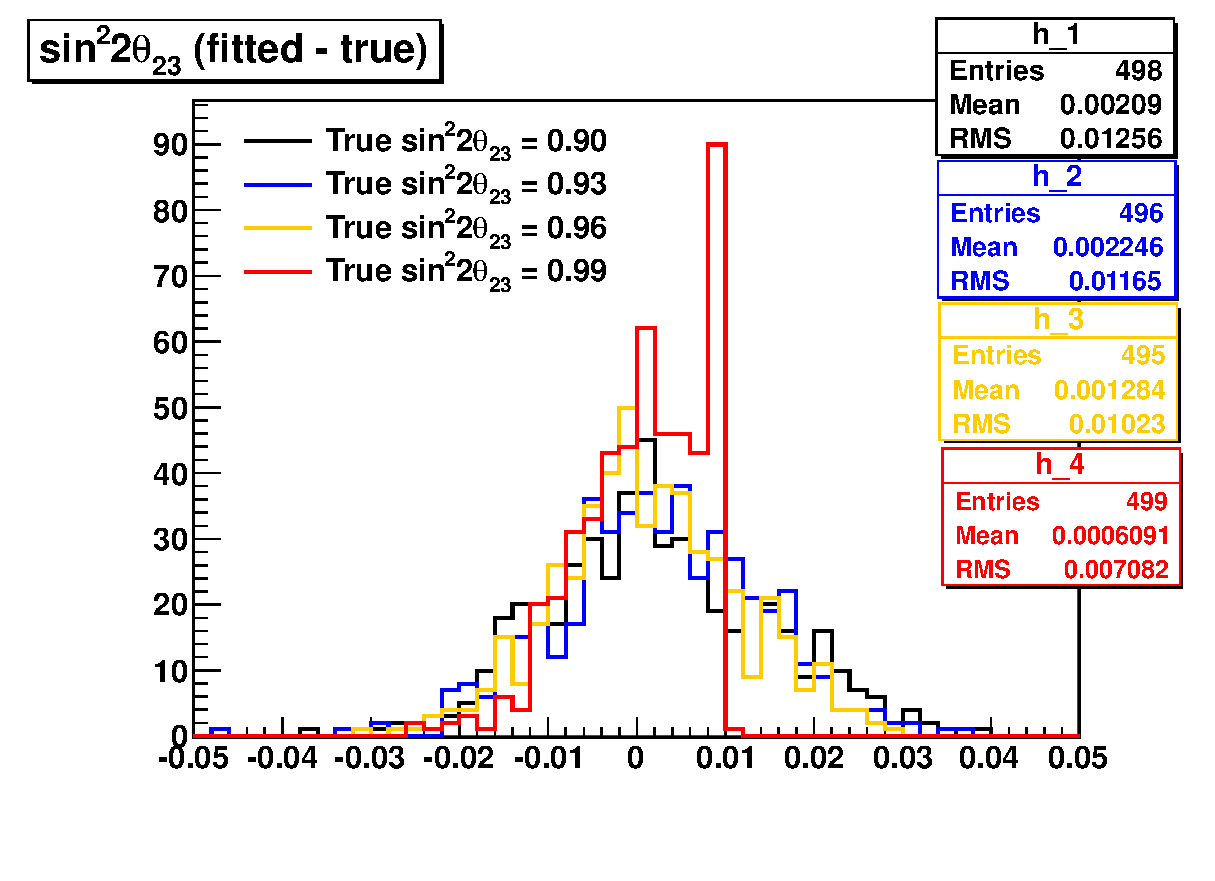
\includegraphics[width=0.5\textwidth]{images/validation/ResidualsSinsq2Theta23.eps}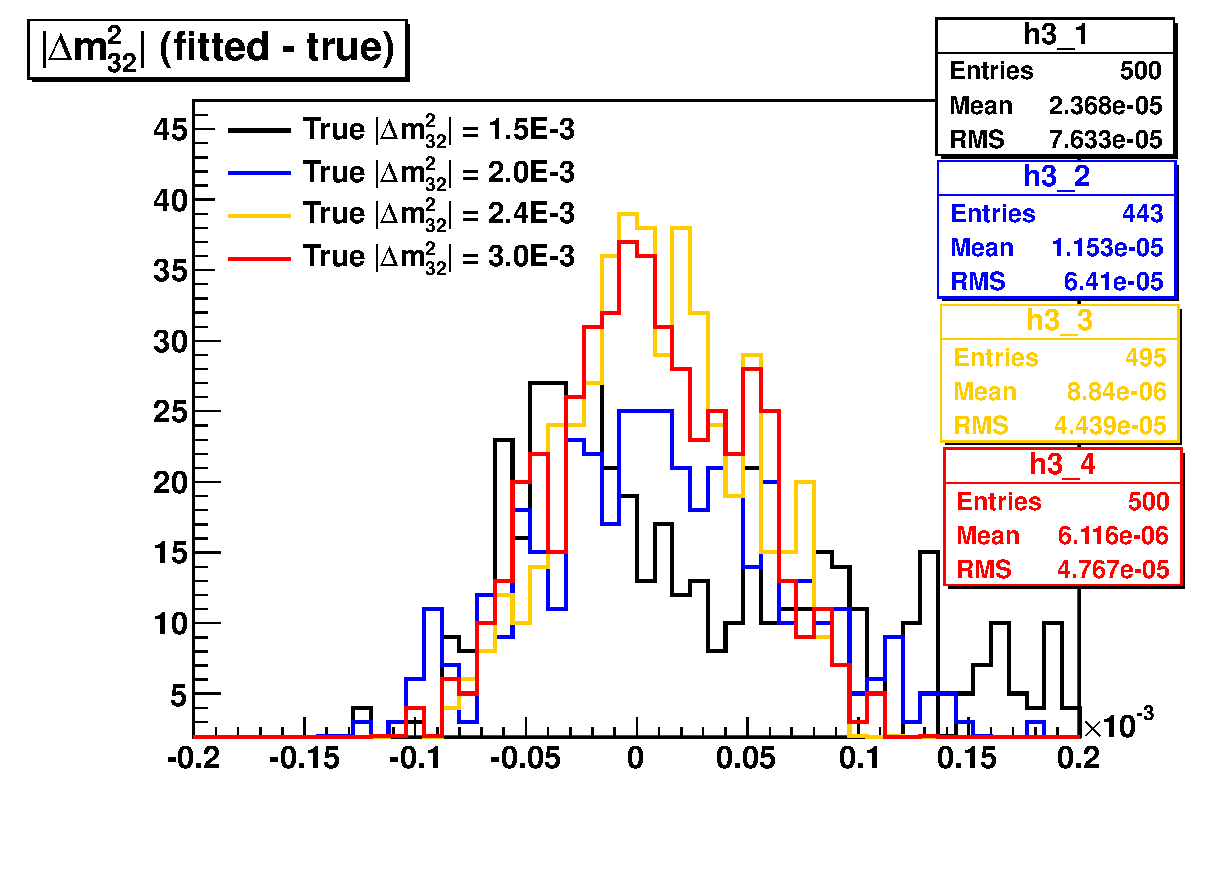
\includegraphics[width=0.5\textwidth]{images/validation/ResidualsDmsq23.eps}
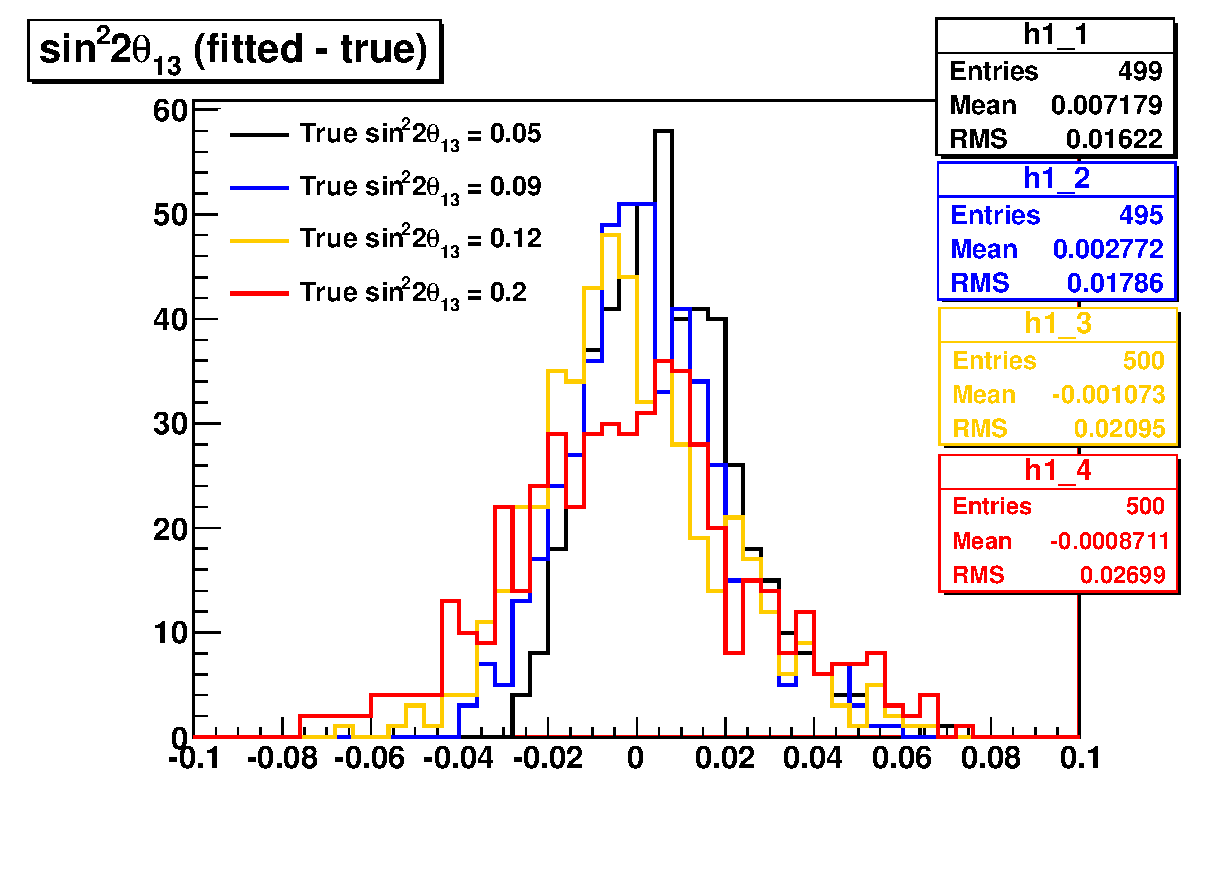
\includegraphics[width=0.5\textwidth]{images/validation/ResidualsSinsq2Theta13.eps}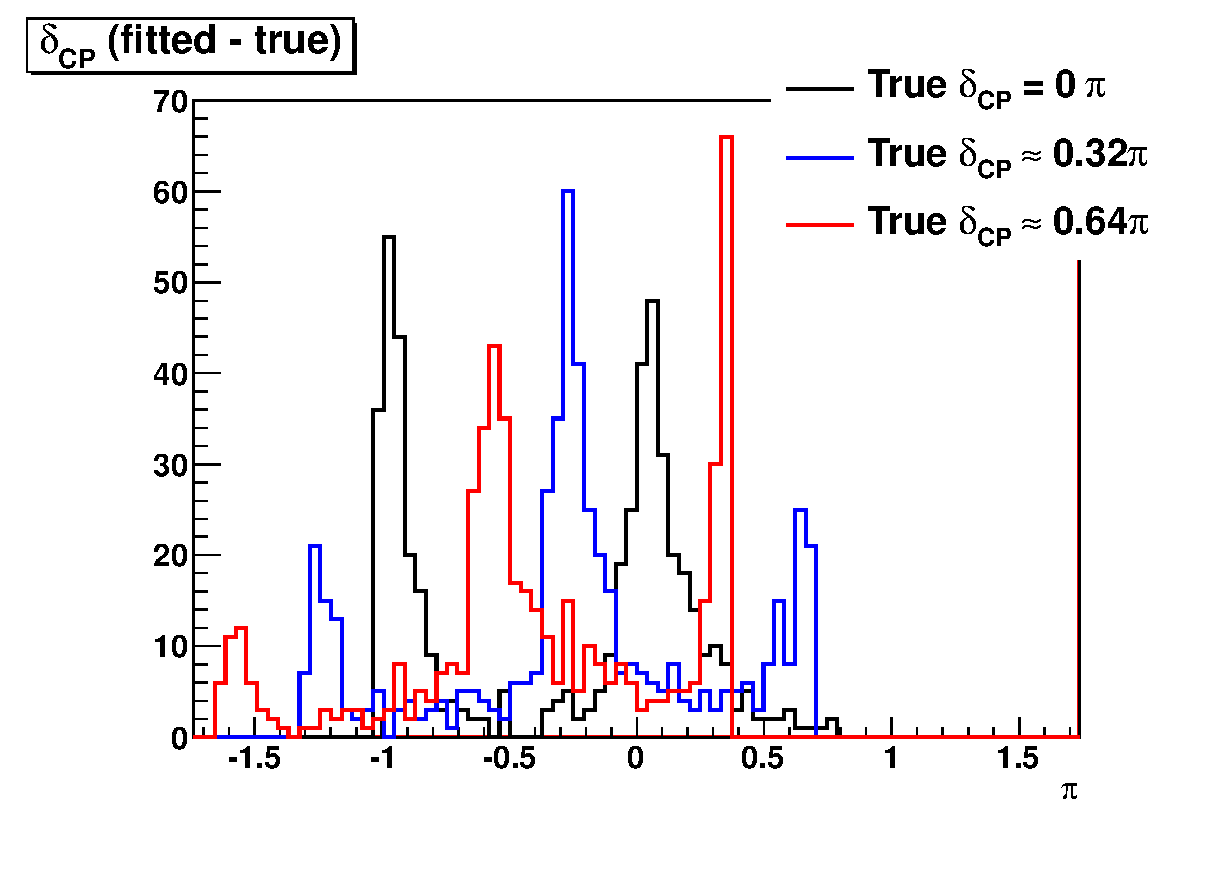
\includegraphics[width=0.5\textwidth]{images/validation/ResidualsDeltaCP.eps}
\caption{Residuals calculated as the difference between the fitted value and the true input value for the estimated final POT, using different sets of values of each of the oscillation parameters. }
\label{fig:res2theta}
\end{center}
\end{figure}

Identical plots of residuals are obtained for current POT. They are presented in figures \ref{fig:residuals2thetacurrtheta23} and \ref{fig:res2thetacurroth}. Plots in figure \ref{fig:residuals2thetacurrtheta23} show the distribution of residuals for the oscillation parameter $sin^{2}2\theta_{23} $ where obvious pile-ups appear in each plot at maximual $sin^{2}2\theta_{23} =1.0$ due to the physical boundary. This effect is more pronounced now with less POT in comparison with \ref{fig:res2theta} because for less POT the distributions are wider in general (more difficult to fit correctly with less events), so more events would be expected to go further  $sin^{2}2\theta_{23} >1.0$, piling up at that maximal value as it is the bound for the fitter. Also, the pile-up effect is more pronounced for larger values of true  $sin^{2}2\theta_{23} $ simply because the true value is closer to the physical boundary. 

\begin{figure}[htbp]
\begin{center}
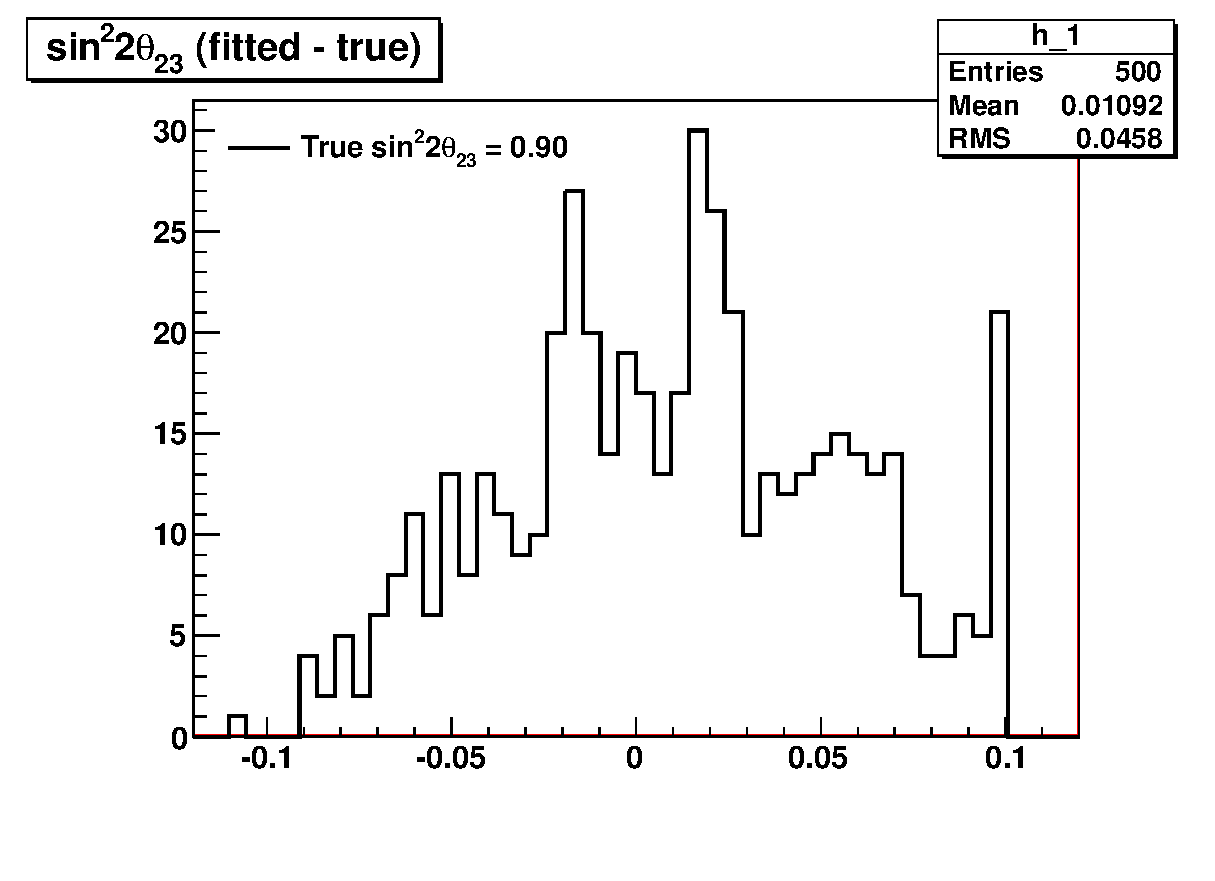
\includegraphics[width=0.5\textwidth]{images/validation/ResidualsSinsq2Theta23Current1.eps}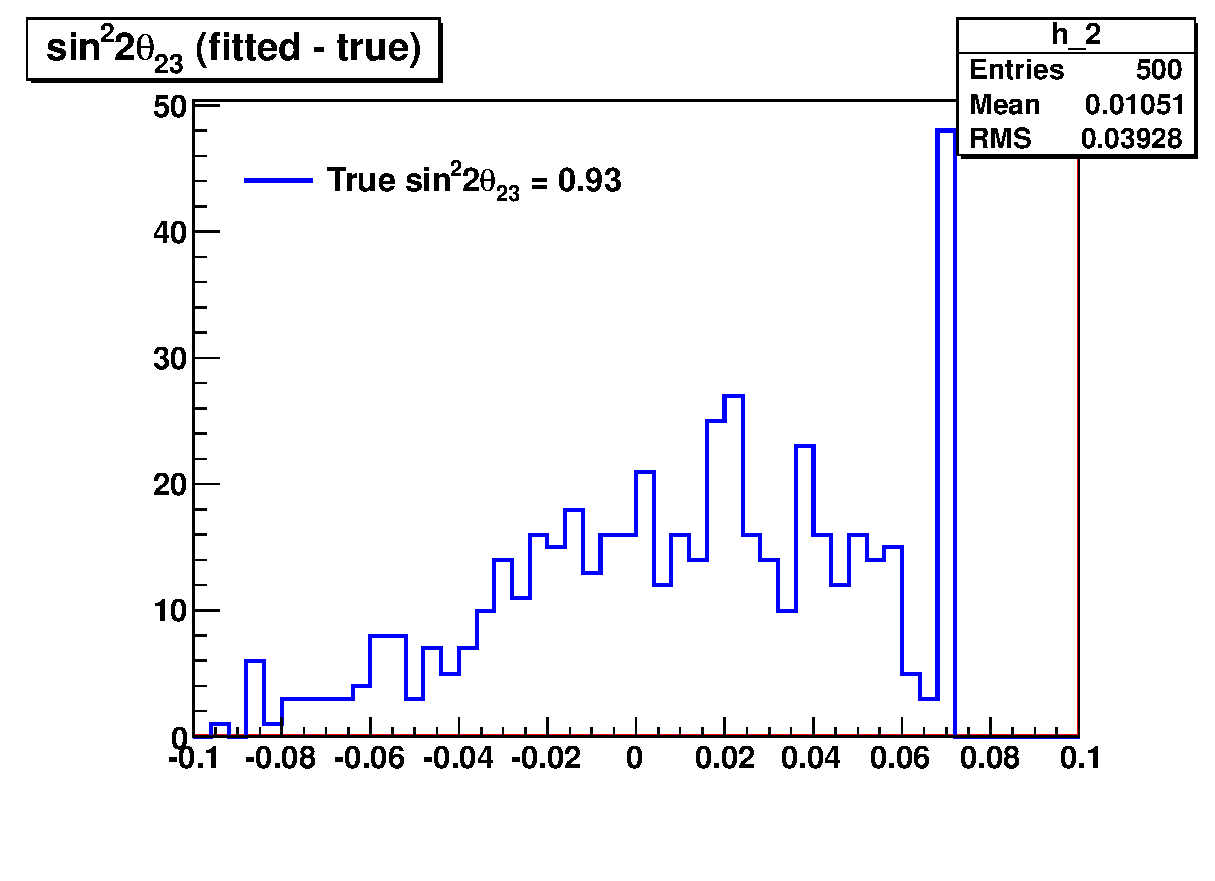
\includegraphics[width=0.5\textwidth]{images/validation/ResidualsSinsq2Theta23Current2.eps}
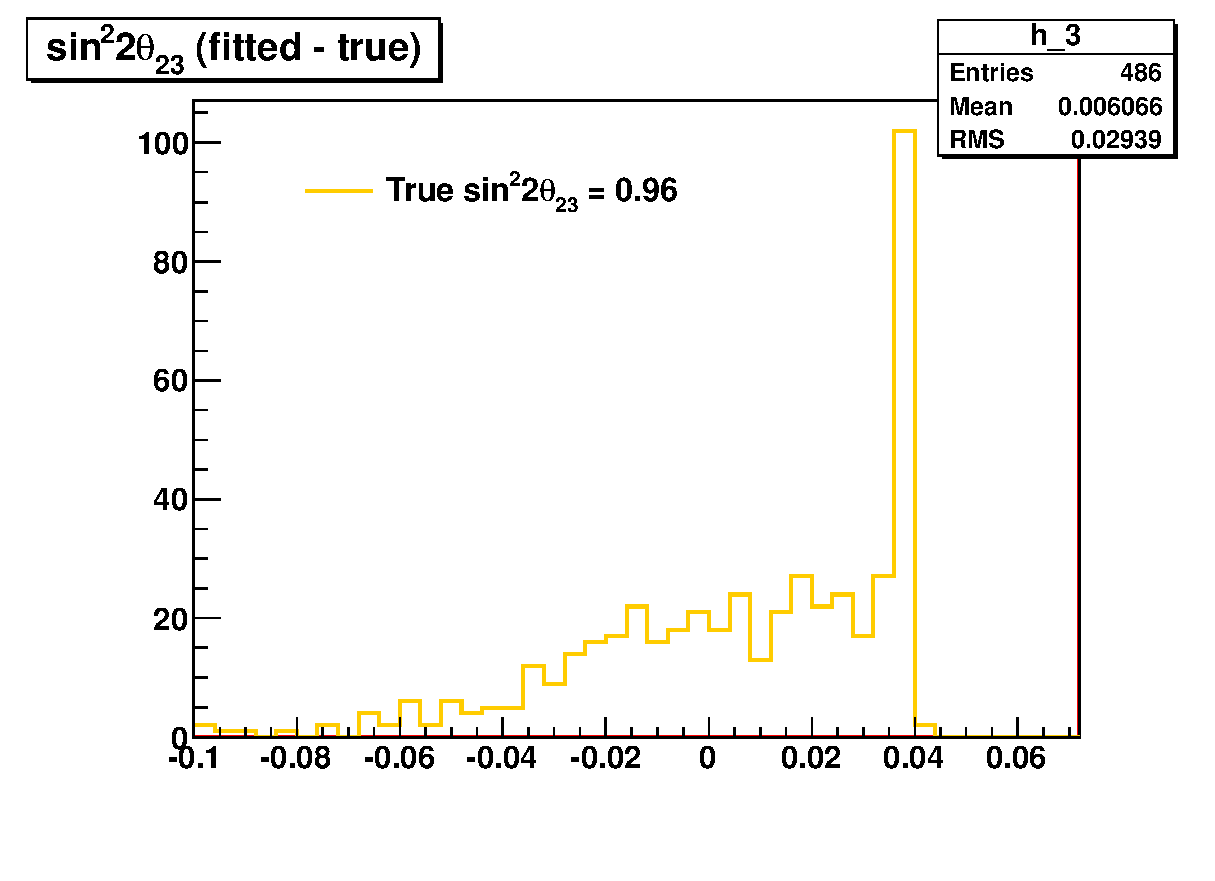
\includegraphics[width=0.5\textwidth]{images/validation/ResidualsSinsq2Theta23Current3.eps}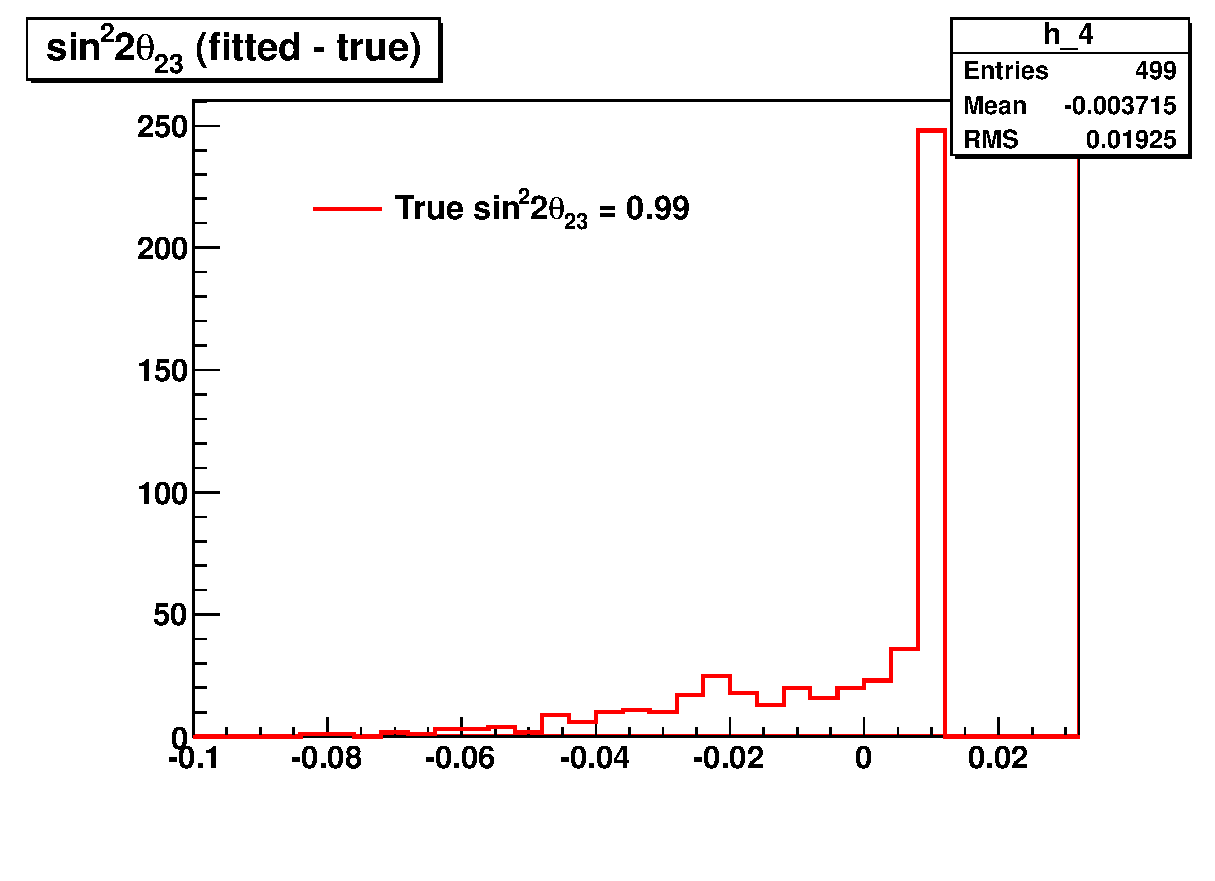
\includegraphics[width=0.5\textwidth]{images/validation/ResidualsSinsq2Theta23Current4.eps}
\caption{Residuals for the oscillation parameter  $sin^{2}2\theta_{23}$  calculated as the difference between the fitted value and the true input value for the current POT, using different values of  the oscillation parameter. }
\label{fig:residuals2thetacurrtheta23}
\end{center}
\end{figure}


\begin{figure}[htbp]
\begin{center}
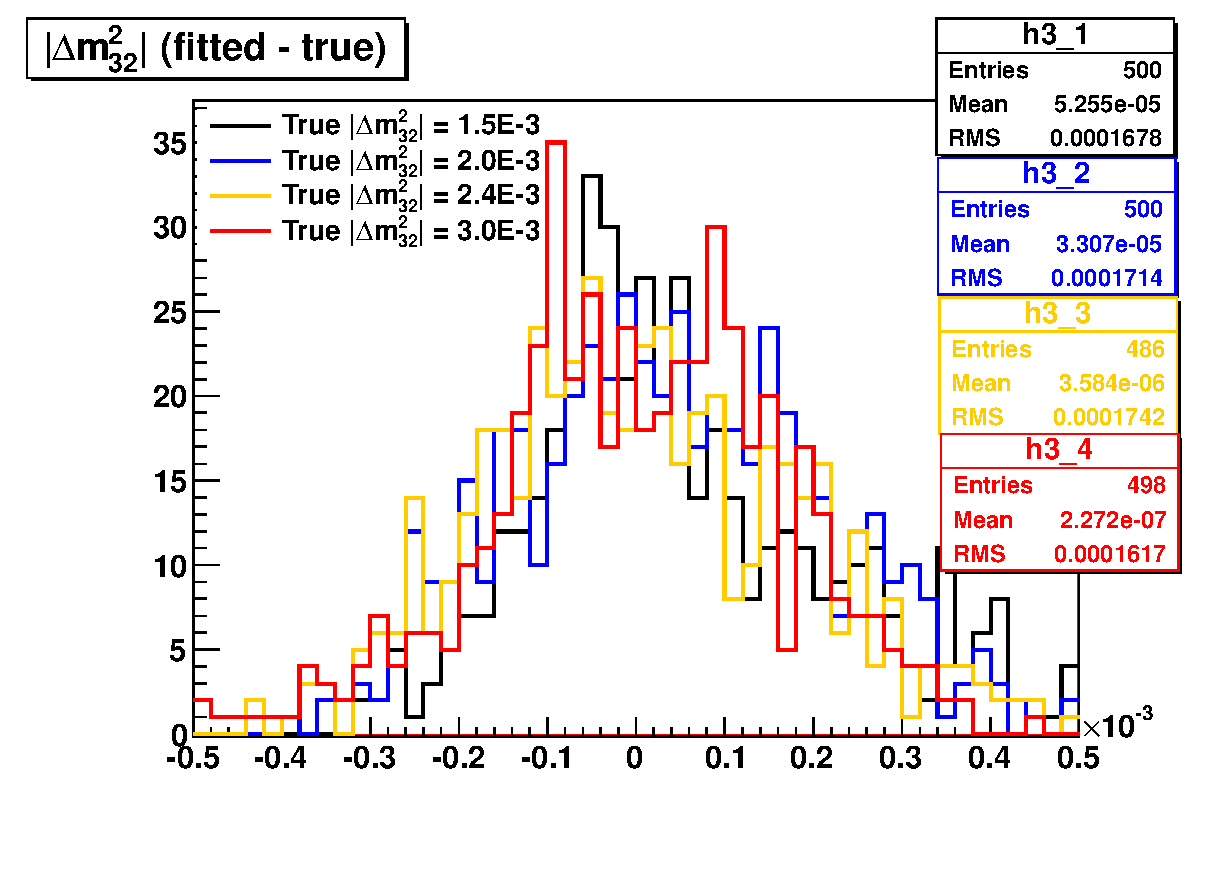
\includegraphics[width=0.5\textwidth]{images/validation/ResidualsSinsq2Dmsq23Current.eps}
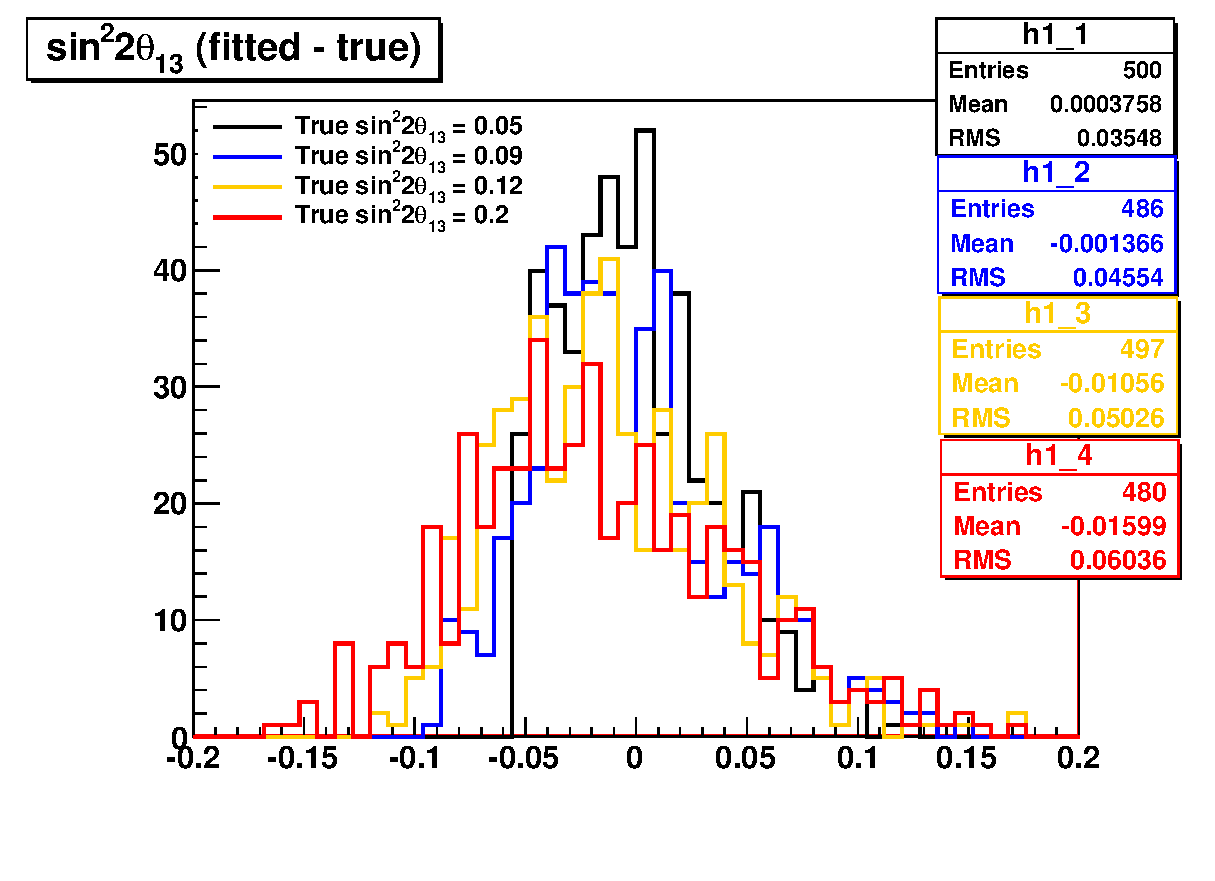
\includegraphics[width=0.5\textwidth]{images/validation/ResidualsSinsq2Theta13Current.eps}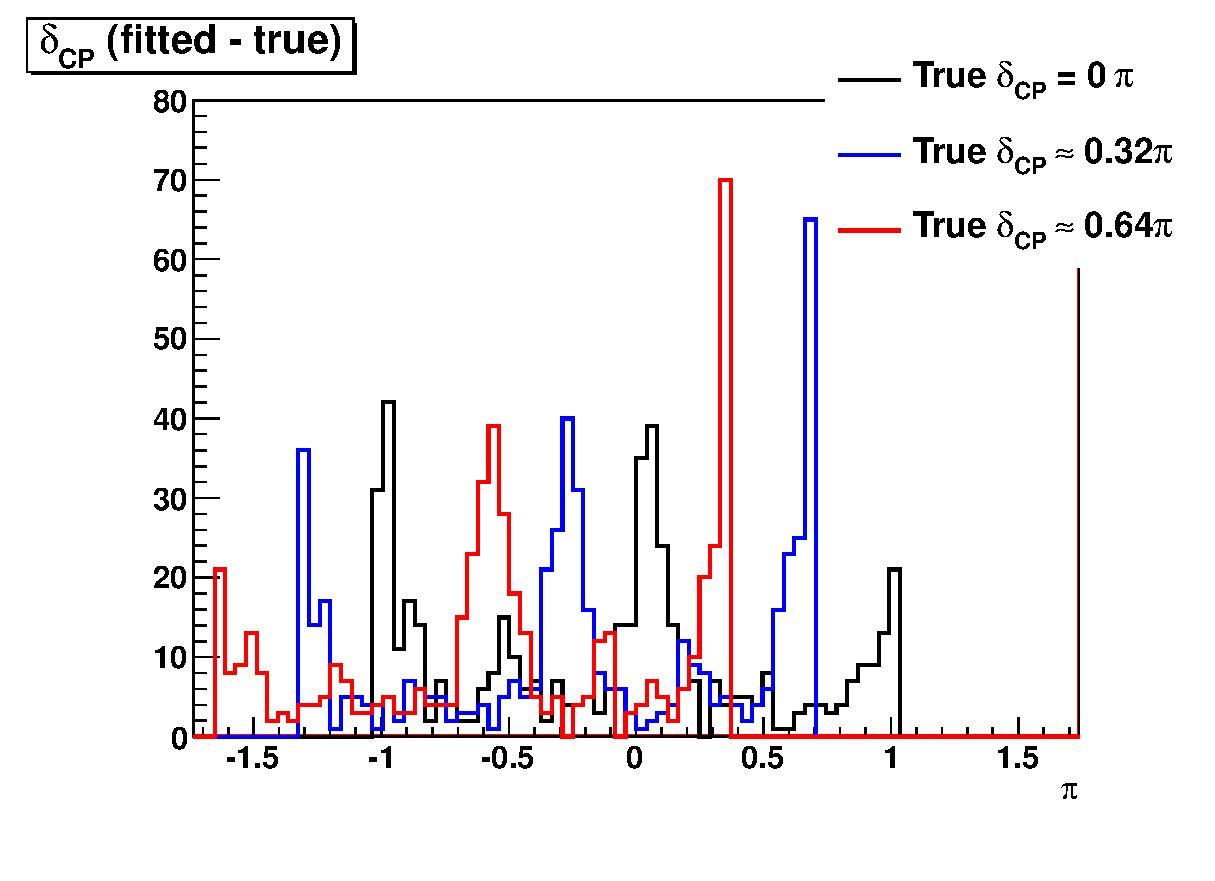
\includegraphics[width=0.5\textwidth]{images/validation/ResidualsDeltaCPCurrent.eps}
\caption{Residuals calculated as the difference between the fitted value and the true input value for the current POT, using different sets of values of each of the oscillation parameters. }
\label{fig:res2thetacurroth}
\end{center}
\end{figure}


The same study of residuals was repeated for $sin^{2}\theta$ variables with the estimated final POT. In this case the study needed a modification due to the dependency of the result with the initial value selected for $sin^{2}\theta_{23}$, so it was necessary to adopt the 2x2 fit as already explained in Sec. \ref{subsec:fitter}. Even with the improved 2x2 fit, the resultant plots for $sin^{2}\theta_{23}$ still present two peaks, one centered at zero (for results in the correct octant) and one biased (for results in the \textit{mirror} octant). Furthermore, both peaks have similar number of events as one can see in figure \ref{fig:residualstheta23}. The pile-up effect also appeared in $sin^{2}\theta_{23}$ distributions when the true input value of that oscillation parameter is close to the center of symmetry (\ref{fig:residualstheta23}, left plot). For a better understanding of the value of the center of symmetry (note that it is not exactly 0.5), see appendix \ref{app:symmetry}.

\begin{figure}[htbp]
\begin{center}
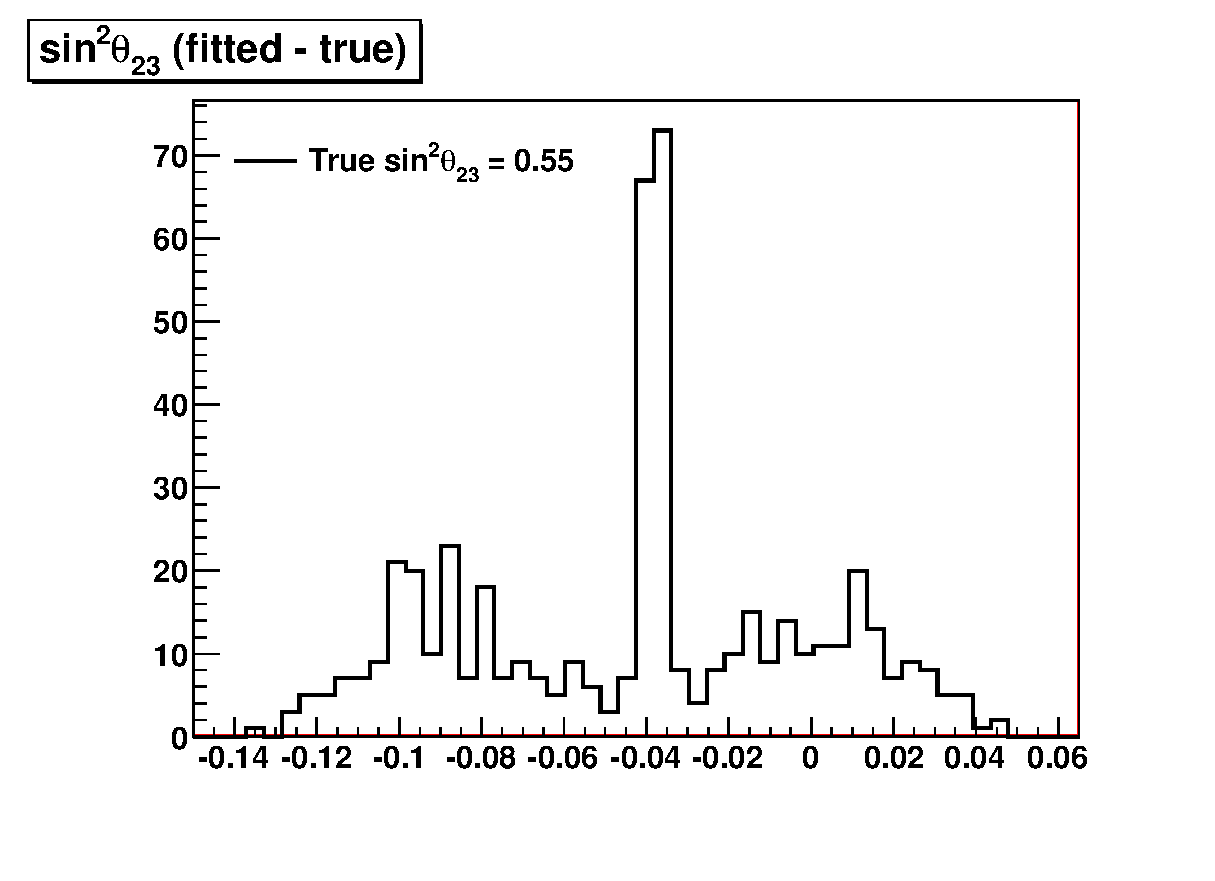
\includegraphics[width=0.35\textwidth]{images/validation/ResidualsSinsqTheta23Set1.eps}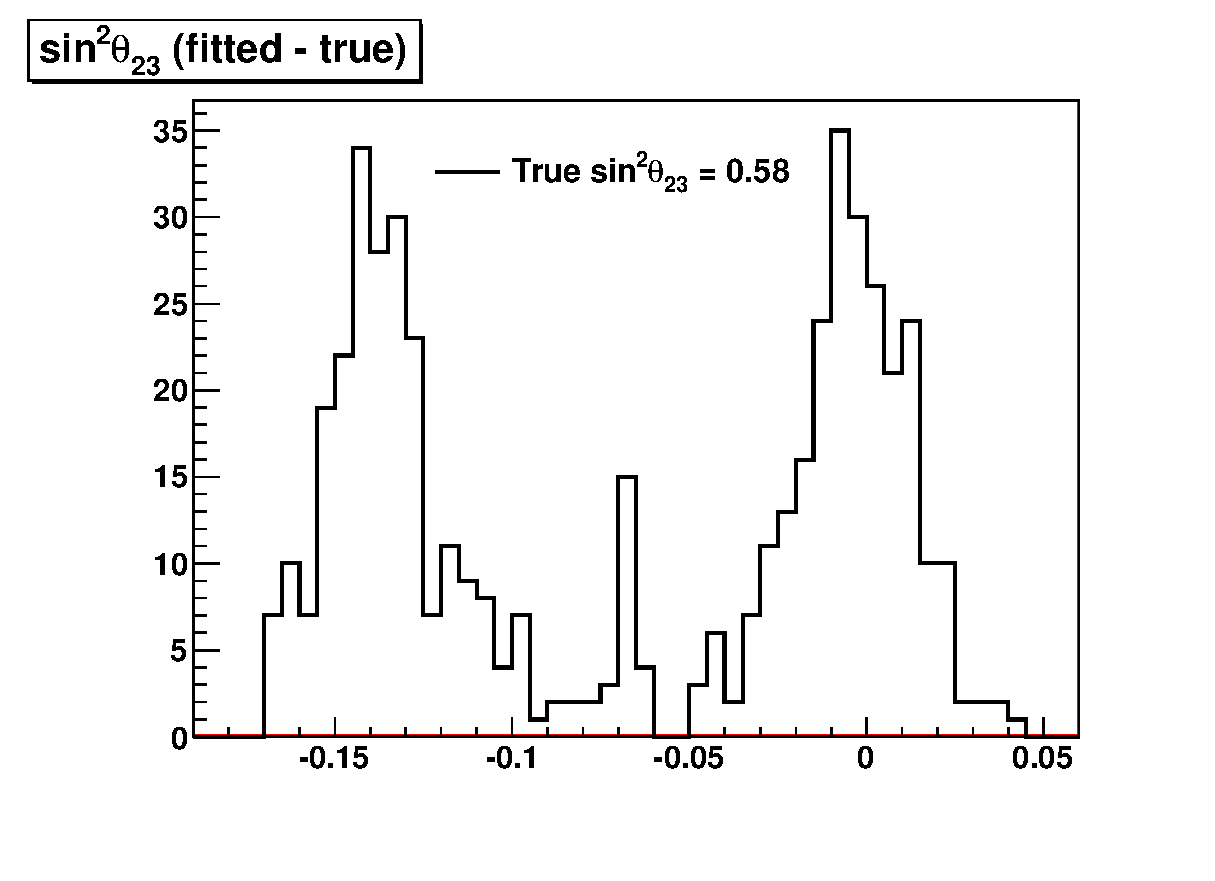
\includegraphics[width=0.35\textwidth]{images/validation/ResidualsSinsqTheta23Set2.eps}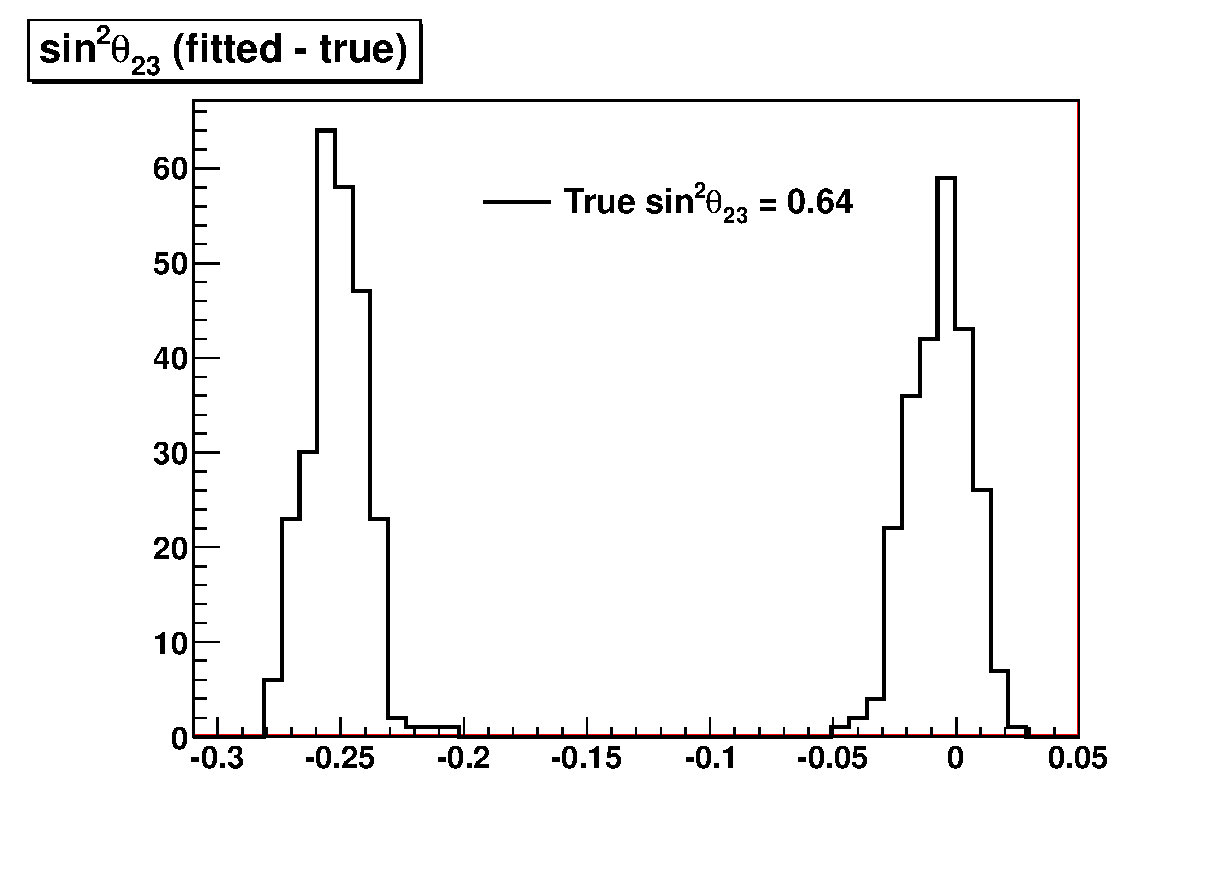
\includegraphics[width=0.35\textwidth]{images/validation/ResidualsSinsqTheta23Set3.eps}
\caption{Residuals for the oscillation parameter  $sin^{2}\theta_{23}$  calculated as the difference between the fitted value and the true input value for the estimated final POT, using different values of that oscillation parameter. }
\label{fig:residualstheta23}
\end{center}
\end{figure}

In order to clarify this behaviour in figure \ref{fig:residualstheta23} it is necessary to look at the other oscillation parameters. In fact, the explanation to the fact that both peaks, in the true and \textit{mirror} octants, still appear is the fitted value of the other angle  $sin^{2}\theta_{13}$. As shown in figure  \ref{fig:residualstheta13theta23} , the fitted value of the angle $sin^{2}\theta_{13}$ is around the true input value for the peak in the true octant for $sin^{2}\theta_{23}$, while for the \textit{mirror} octant, where $sin^{2}\theta_{23}$ is fitted to an incorrect value, the angle  $sin^{2}\theta_{13}$  is also fitted to an incorrect value. This is another clear evidence of the dependency between both angles. 

 \begin{figure}[htbp]
\begin{center}
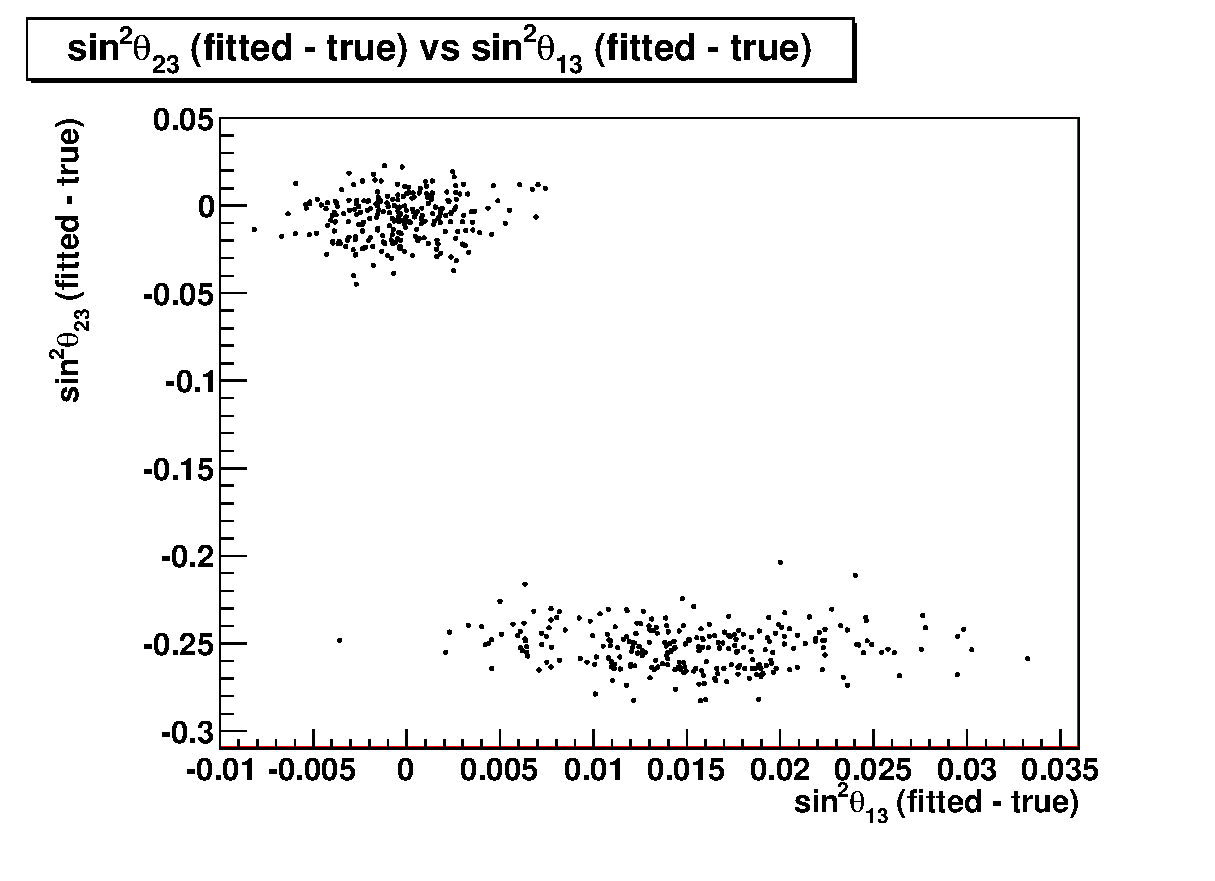
\includegraphics[width=0.7\textwidth]{images/validation/ExampleTheta23Theta13OctantsSet4.eps}
\caption{Example of residuals for $sin^{2}\theta_{23}$ vs $sin^{2}\theta_{13}$ for $sin^{2}\theta_{23}=0.46$ for the estimated final POT. There is a clear separation in two clouds of points centered at two different values for $sin^{2}\theta_{13}$, one at the correct value corresponding to the correct value for $sin^{2}\theta_{23}$ as well, and a biased value corresponding to the \textit{mirror} or incorrect value for $sin^{2}\theta_{23}$. }
\label{fig:residualstheta13theta23}
\end{center}
\end{figure}

Taking now one of the values in figure \ref{fig:residualstheta23}, for instance $sin^{2}\theta_{23}=0.64$, the effect of constraining the other angle $sin^{2}\theta_{13}$ can be checked. In figures \ref{fig:residualstheta13theta23const} and \ref{fig:residualstheta13const} the constraint in $sin^{2}\theta_{13}$ was done through a penalty term as explained in \ref{sec:chisq} where the mean value is set to $sin^{2}\theta_{13}=0.09$, i.e. the true input value, and the error is set to 20\%. As expected, when constraining the angle $sin^{2}\theta_{13}$, the peak in the \textit{mirror} octant for $sin^{2}\theta_{23}$, i.e. the events with an incorrect fitted $sin^{2}\theta_{23}$ disappear. Also, looking at \ref{fig:residualstheta13const} it is clear that the distribution for $sin^{2}\theta_{13}$ is biased presenting two peaks before constraining, disappearing such bias when the constraint in $sin^{2}\theta_{13}$ is applied. 

 \begin{figure}[htbp]
\begin{center}
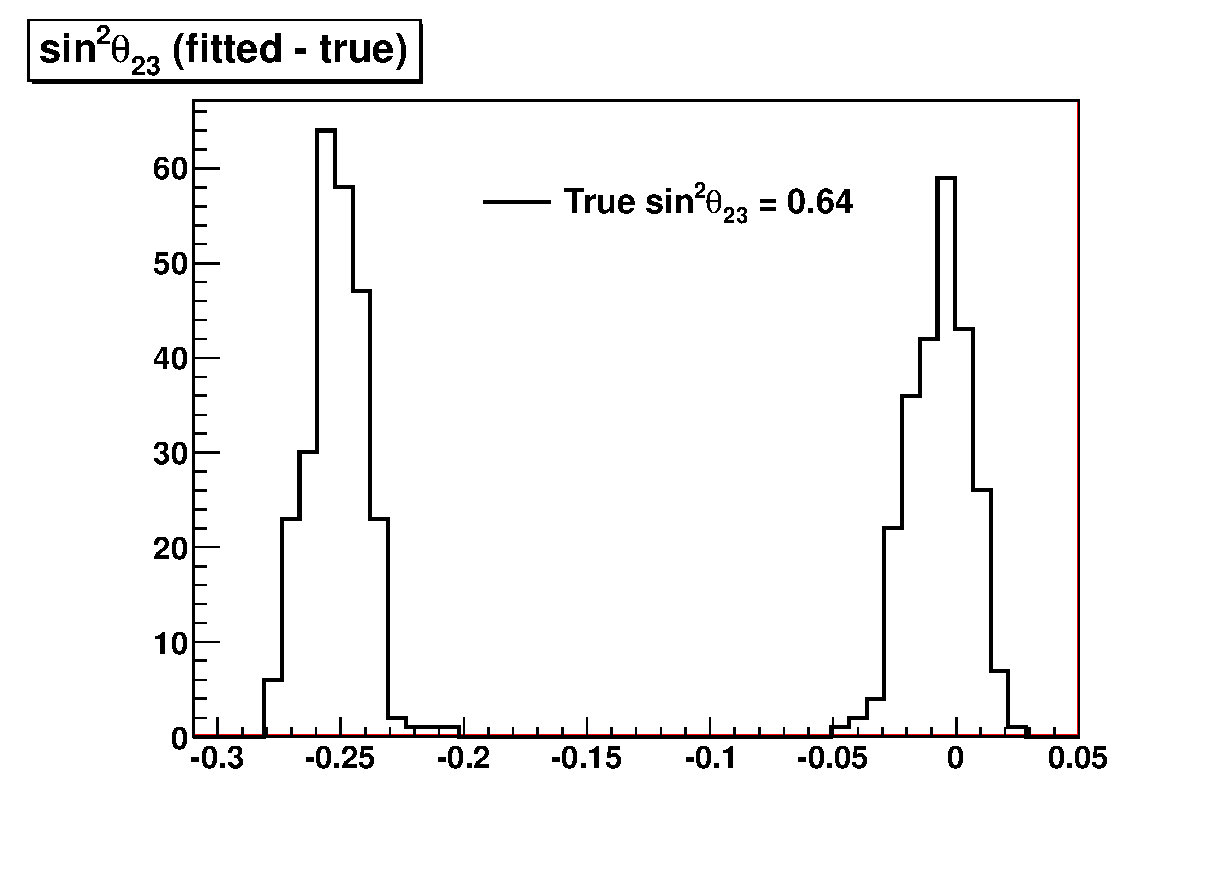
\includegraphics[width=0.5\textwidth]{images/validation/ResidualsSinsqTheta23Set3.eps}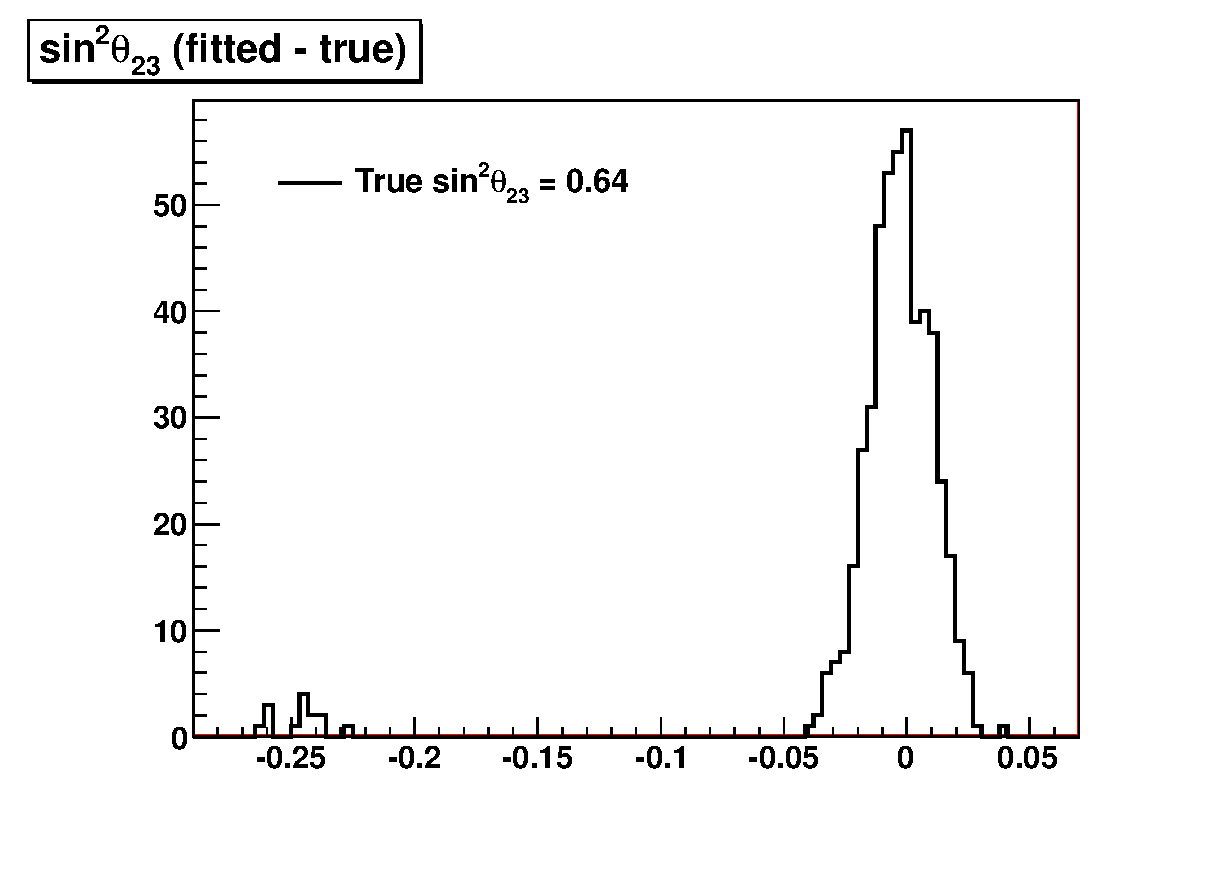
\includegraphics[width=0.5\textwidth]{images/validation/ResidualsSinsqTheta23Set3Constrain.eps}
\caption{Example of the effect of constraining the angle $sin^{2}\theta_{13}$ around its true input value with a 20\% error in the distribution of residuals for $sin^{2}\theta_{23}=0.64$ for the estimated final POT. The plot before constraining (left) shows the two symmetric peaks, while after constraining (right) the peak in the incorrect octant disappeared. }
\label{fig:residualstheta13theta23const}
\end{center}
\end{figure}

\begin{figure}[htbp]
\begin{center}
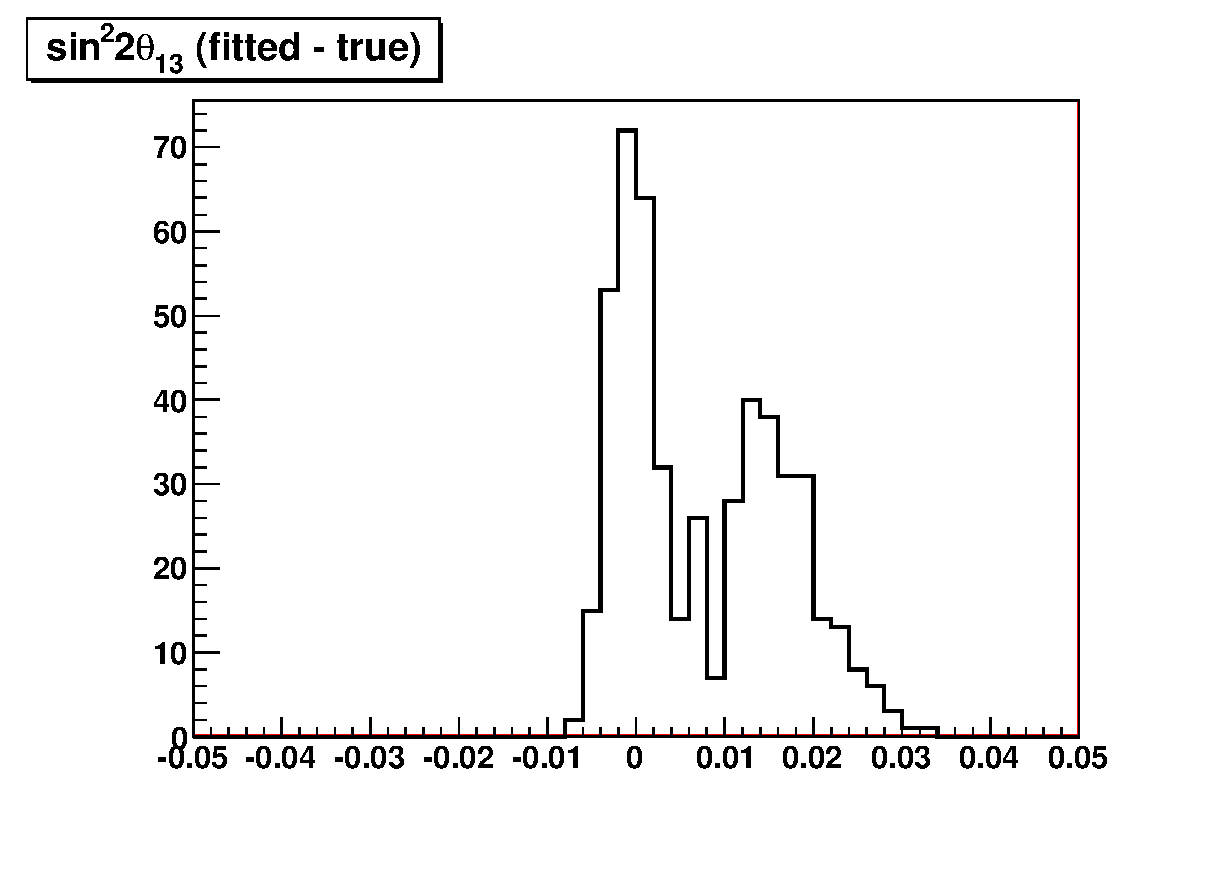
\includegraphics[width=0.5\textwidth]{images/validation/ResidualsSinsqTheta13BeforeConstraining.eps}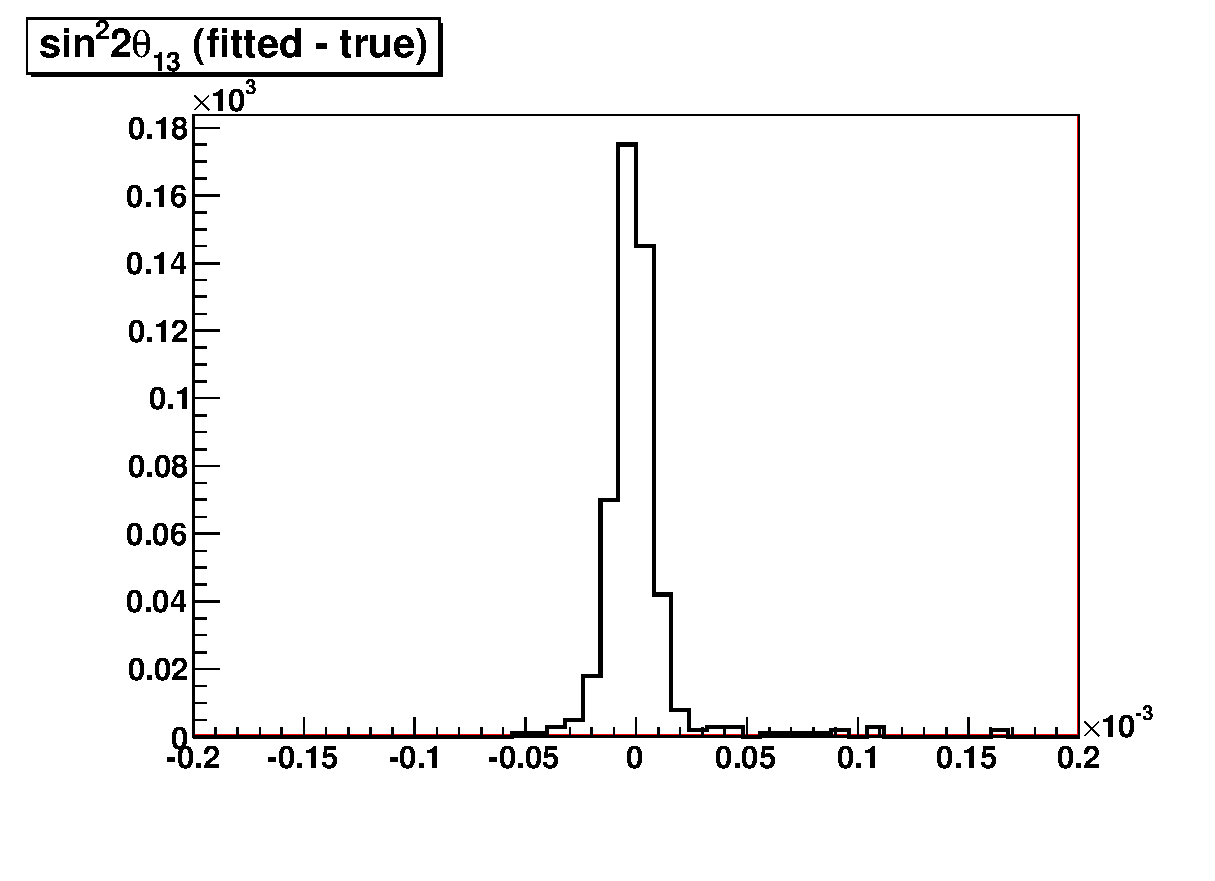
\includegraphics[width=0.5\textwidth]{images/validation/ResidualsSinsqTheta13AfterConstraining.eps}
\caption{Example of the effect of constraining the angle $sin^{2}\theta_{13}$ around its true input value with a 20\% error in the distribution of residuals for $sin^{2}\theta_{13}=0.64$ for the estimated final POT. The plot before constraining (left) shows a clear biased distribution with two peaks, while after constraining (right) the distribution is correctly centered around zero. }
\label{fig:residualstheta13const}
\end{center}
\end{figure}

The effect of constraining the angle $sin^{2}\theta_{13}$ can be studied in more detail when looking at the distribution of one ring $\mu$-like events and the number or one ring e-like events. Figure \ref{fig:rdistributionconst} presents the $E_{reco}$ distribution of  one ring $\mu$-like events in the first octant for one example toy experiment with value of  $sin^{2}\theta_{23}=0.64$ with and without constraining $sin^{2}\theta_{13}$ (left plot) and the ratio between both distributions, with and without constraining $sin^{2}\theta_{13}$ (right plot). Table \ref{tab:effconst} shows the effect of constraining $sin^{2}\theta_{13}$ in the total predicted number of events for the one ring $\mu$-like and e-like events. In conclusion, both the appearance contribution (predicted number of one ring e-like events) and the disappearance contribution (predicted number and $E_{reco}$ distribution of one ring $\mu$-like events) are affected when constraining the angle $sin^{2}\theta_{13}$, being for the $E_{reco}$ distribution of one ring $\mu$-like events larger the effect at low momentum, around the oscillation maximum. 

 \begin{figure}[htbp]
\begin{center}
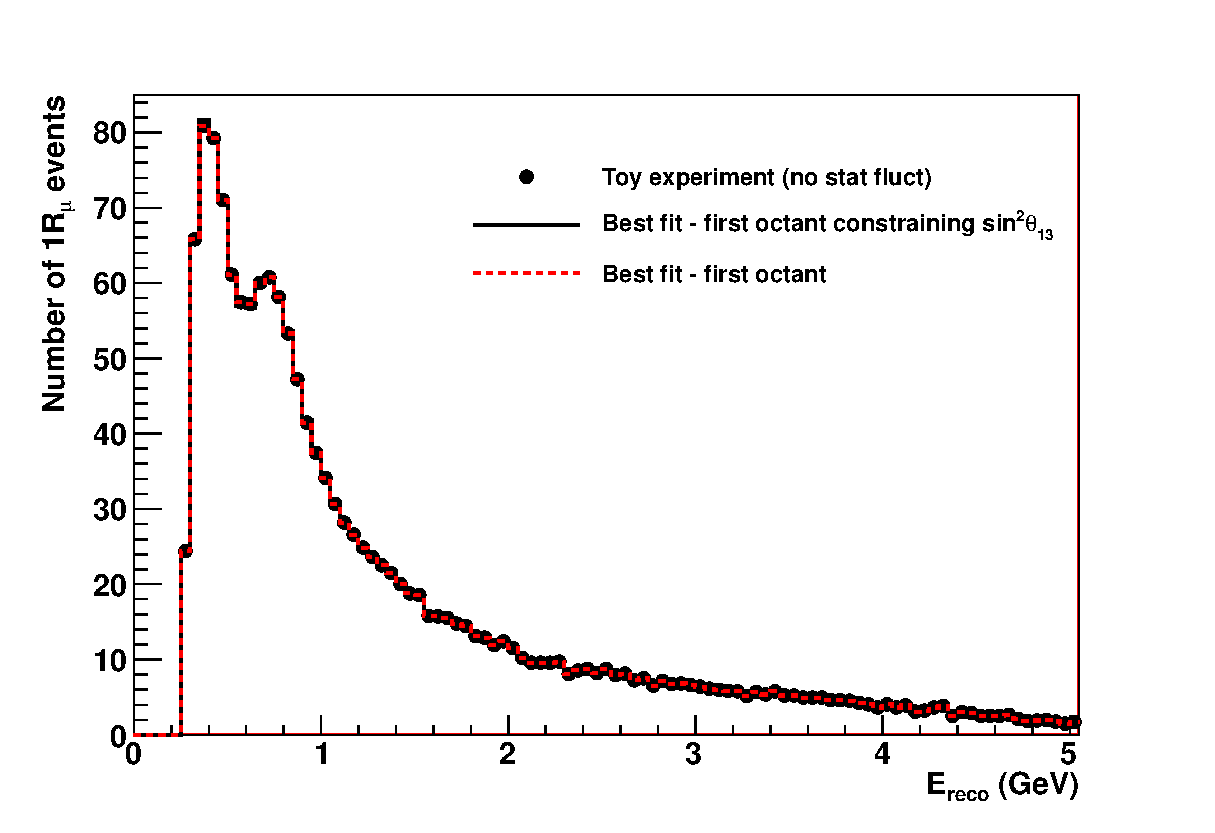
\includegraphics[width=0.5\textwidth]{images/validation/ExampleDistributionFirstOctantConstrain.eps}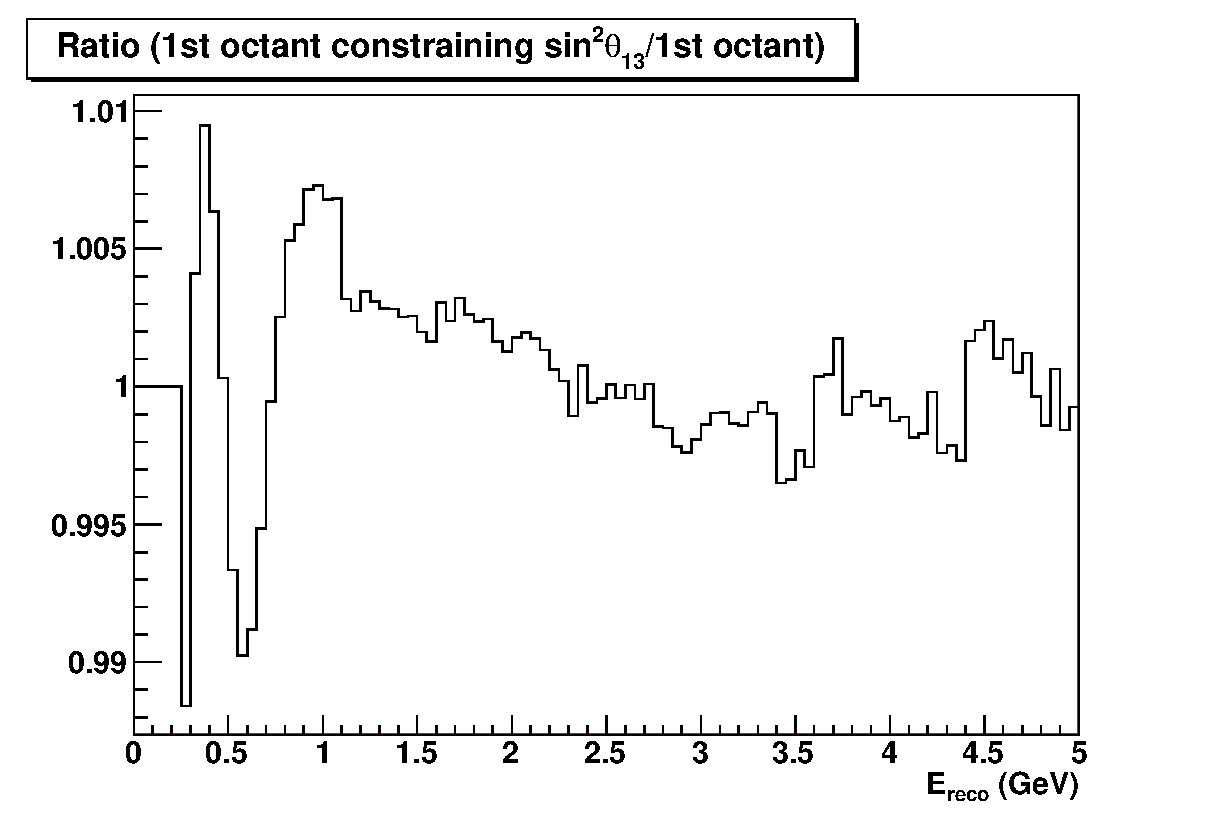
\includegraphics[width=0.5\textwidth]{images/validation/ExampleDistributionFirstOctantConstrainRatio.eps}
%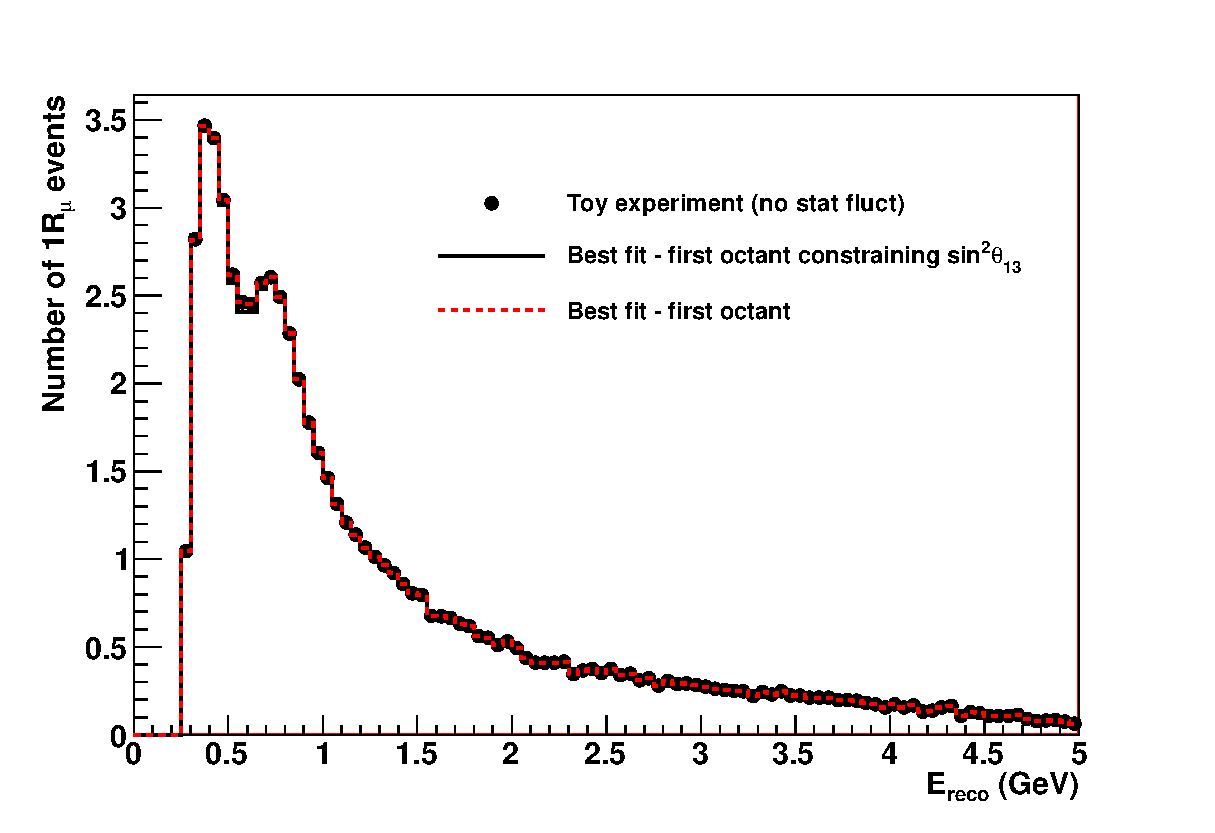
\includegraphics[width=0.5\textwidth]{images/validation/ExampleDistributionFirstOctantConstrainCurrent.eps}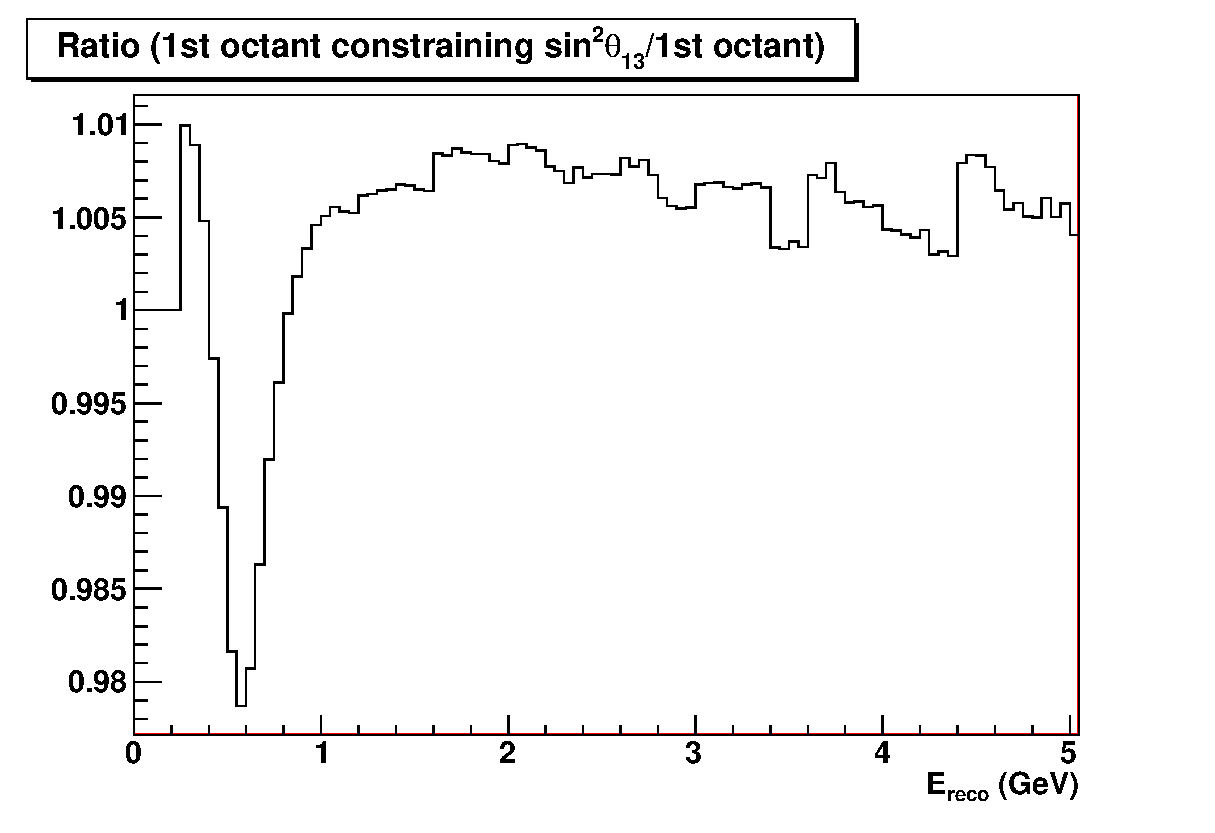
\includegraphics[width=0.5\textwidth]{images/validation/ExampleDistributionFirstOctantConstrainRatioCurrent.eps}
\caption{$E_{reco}$ distribution of  one ring $\mu$-like events in the first octant for one example toy experiment with value of  $sin^{2}\theta_{23}=0.64$ for the estimated final POT with and without constraining $sin^{2}\theta_{13}$ (left plot) and the ratio between both distributions, with and without constraining $sin^{2}\theta_{13}$ (right plot). }%For estimated final POT (top plots) and current POT (bottom plots). }
\label{fig:rdistributionconst}
\end{center}
\end{figure}

\begin{table}[h]
\centering
\begin{tabular}{|c|c|c|c|}
\hline
 & Total $1R_{\mu}$ events & Total $1R_{e}$ events\\
\hline \hline
Toy experiment & 1607.7 & 272.3 \\
Best fit, \textit{mirror} octant & 1607.7 & 272.3 \\
Best fit, \textit{mirror} octant, constraining $sin^{2}\theta_{13}$ & 1609.6 &  269.0\\
\hline
\end{tabular}
\caption{Initial values for each oscillation parameter and the bound values for the fitter. Last row shows the general initial and limit values for the systematic error parameters. }
\label{tab:effconst}
\end{table}

For the other two oscillation parameters, $\delta_{CP}$ and  $\Delta m_{32}^{2}$ nothing was changed when using $sin^{2}\theta$ variables so their distributions look exactly as for figures \ref{fig:res2theta} and \ref{fig:res2thetacurroth}. 

Finally, as an example, the distribution of fitted values for the different systematic parameters is presented in Fig. \ref{fig:systfit} for a particular set of oscillation parameters values ($\delta_{CP}=0$, $sin^{2}2\theta_{13}=0.09$, $\Delta m_{32}^{2}=2.4\times10^{-3}eV^{2}/c^{4}$, $sin^{2}2\theta_{23}=0.96$). Those distribution plots allowed to test the bounds for the fitter for the systematics and finally set them to ($-\sigma, \sigma$).

 \begin{figure}[htbp]
\begin{center}
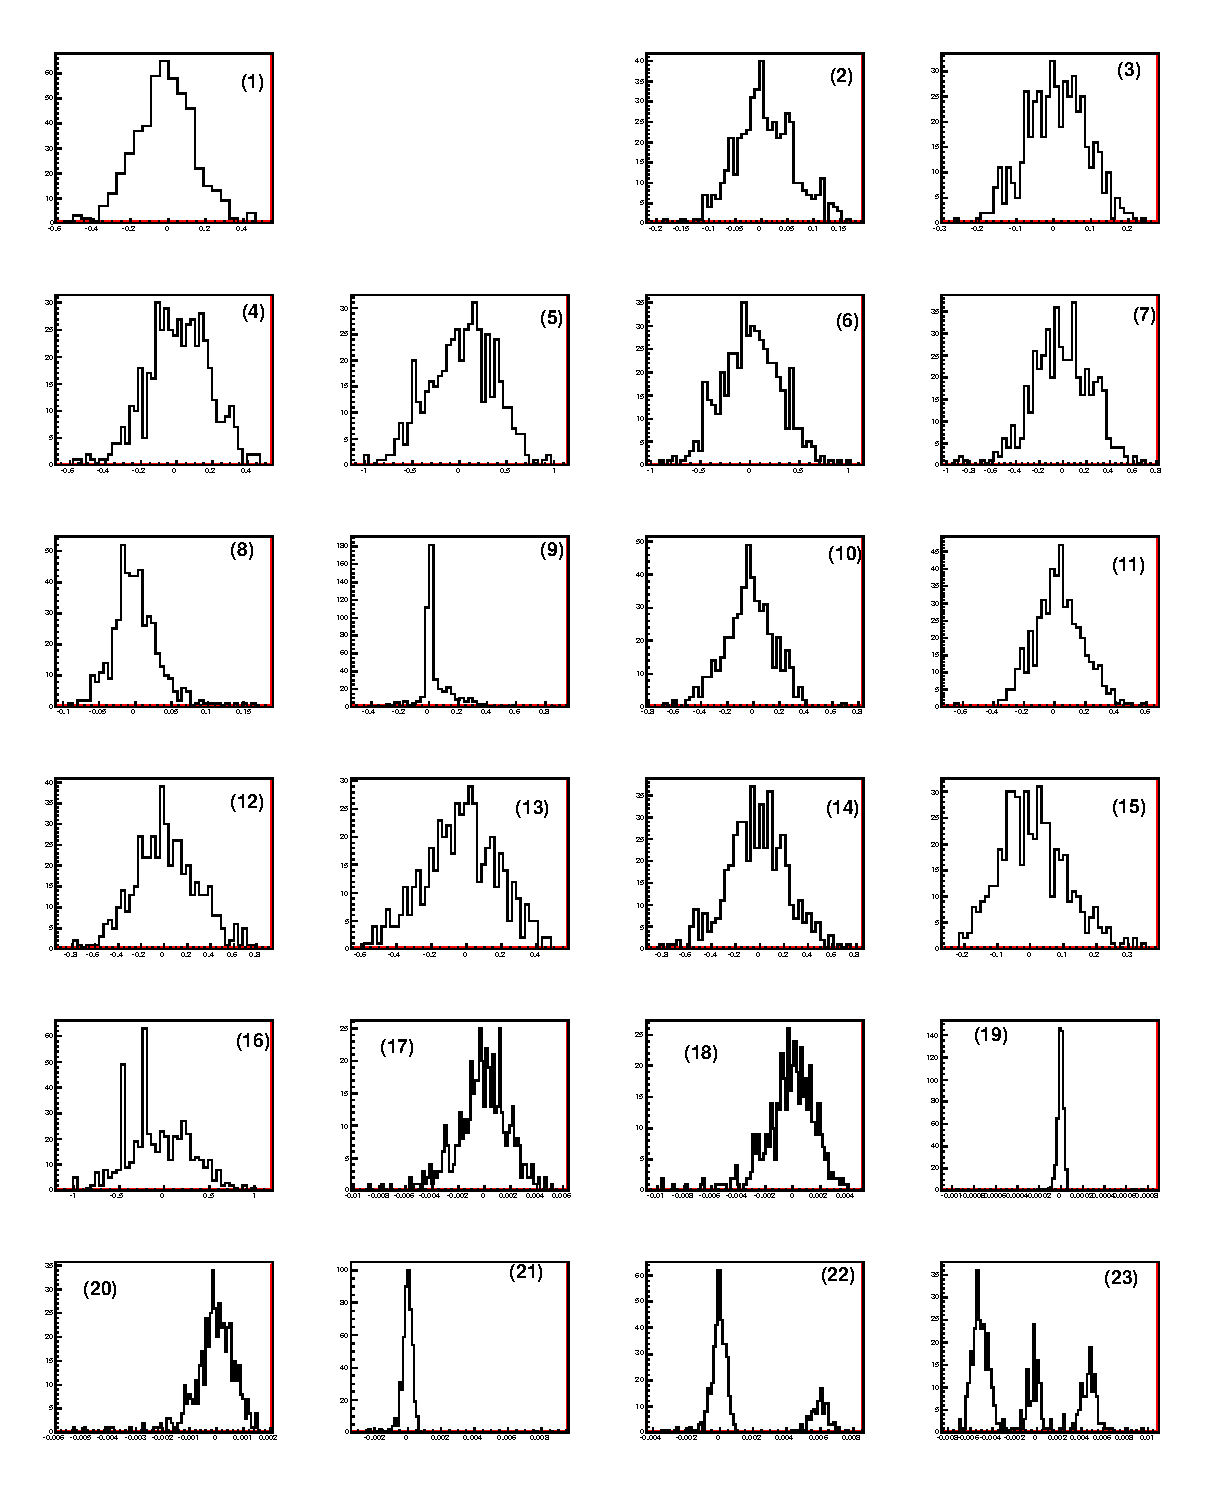
\includegraphics[width=1.0\textwidth]{images/validation/ExampleResidualsSystematics.eps}
\caption{ Distribution of fitted values for the different systematic parameters for a particular set of oscillation parameters values ($\delta_{CP}=0$, $sin^{2}2\theta_{13}=0.09$, $\Delta m_{32}^{2}=2.4\times10^{-3}eV^{2}/c^{4}$, $sin^{2}2\theta_{23}=0.96$) for the estimated final POT. Systematics are: (1) Flux shape, (2) 1R$_{\mu}$ CCQE efficiency, (3), (4) and (5) 1R$_{\mu}$ CCQE ring counting efficiency, (6) 1R$_{\mu}$ CC non QE efficiency, (7) 1R$_{\mu}$ NC efficiency, (8) 1R$_{\mu}$ $\nu_{e}$ CC efficiency, (9) Energy scale, (10) ND280 efficiency,  (11) Flux normalization, (12) CCQE cross section, (13) CC1$\pi$ to CCQE cross section, (14) CC other to CCQE cross section, (15) NC to CCQE cross section, (16) Nuclear Effect, (17) 1R$_{e}$ signal efficiency, (18) 1R$_{e}$ background efficiency, (19) CC coh to CCQE efficiency, (20) NC 1$\pi$0 to CCQE cross section, (21) NC coh to CCQE cross section, (22) NC other to CCQE cross section, (23) $\nu_{e}$ to $\nu_{\mu}$ cross section. }
\label{fig:systfit}
\end{center}
\end{figure}


%%%%%%%%%%%%%%%%%%%%
%%%% Sensitivity studies %%%%%%%%%
\subsection{Sensitivity studies}

In this section several sensitivity plots will be presented, including 1D marginalized $\Delta\chi^{2}$ distributions and 2D confidence regions.

For the 1D marginalized $\Delta\chi^{2}$ distributions vs each of the oscillation parameters, the selected oscillation parameter is scanned, so in each bin the other three oscillation parameters and the systematic parameters are fitted, being finally the value of $\chi^{2}$ after the fit in each bin the one used to build the $\Delta\chi^{2} = \chi^{2} - \chi^{2}_{min}$ distribution. 

For the plots showing 2D confidence regions each 2D phase space is scanned in terms of a given binning which is summarized in table \ref{tab:binning}. For each grid point (temporary fixed two oscillation parameters) the other two oscillation parameters (four when solar parameters are fitted as well) are marginalized by the fitter along with the systematic parameters, resulting in a final value of $\chi^{2}$ in each grid point. The fitted value of the other two (four) oscillation parameters is presented in a 3D color plot together with each 2D contour. Notice that all the contours presented in this subsection are done at an estimation of the final POT. 

\begin{table}[h]
\centering
\begin{tabular}{|c|c|c|c|c|}
\hline
 Parameter & Minimum & Maximum & Step & \# bins\\
\hline \hline
$sin^{2}2\theta_{23}$ & 0.9 & 1.0 & 0.002 & 50\\
$sin^{2}2\theta_{13}$ & 0.0 & 0.264 & 0.008 & 33 \\
$\Delta m_{32}^{2} (\times 10^{-3} eV^{2}/c^{4})$ & 2.0& 3.0& 0.05 & 50 \\
$\delta_{CP}$ & -$\pi$ & $\pi$& $\frac{2\pi}{50}$ & 50\\
\hline
\end{tabular}
\caption{Summary of the binning used for the 2D contours in the validation step. }
\label{tab:binning}
\end{table}


\subsubsection{Sensitivity plots for the joint oscillation analysis}

The 1D marginalized $\Delta\chi^{2}$ distributions for the four oscillation parameters allow us to check several aspects. First of all, the position of the minimum of $\Delta\chi^{2}$ can be checked against the true input value for the oscillation parameter. Also, the existence of only one minimum (with the exception of $sin^{2}\theta_{23}$ case) can be checked. And finally a search for oddities, spikes and spurious points can be performed.The following test was done for each oscillation parameter, with several different true input values, in the two POT configurations (current and estimated final). No statistical fluctuations are taking into account since one distribution (one line) is to be checked, clearer than a cloud of different lines. 

In figures \ref{fig:1Dchisqtheta23}, \ref{fig:1Dchisqtheta13}, \ref{fig:1Dchisqdm23sq}  and \ref{fig:1Dchisqdeltacp} the 1D marginalized $\Delta\chi^{2}$ distribution for the joint oscillation analysis is presented vs $sin^{2}\theta_{23}$, $sin^{2}\theta_{13}$, $\Delta m_{32}^{2}$ and $\delta_{CP}$ respectively. In each distribution several toy experiments with different true input values of each parameter are presented. In all of them, the different true values for the parameter scanned are written on each plot, and the rest of parameters not scanned have a true value fixed to the following values: $sin^{2}\theta_{23}=0.56$, $sin^{2}\theta_{13}=0.024$,  $|\Delta m_{32}^{2}| = 2.4 \times 10^{-3} eV^{2}/c^{4}$ and $\delta_{CP}=0$. From the plots it is clear the good recovery of the true input value by the fitter (at the minimum). The two minima (symmetry values) appear as expected for $sin^{2}\theta_{23}$. 

Comparing in \ref{fig:1Dchisqtheta23} the plots with different values of  $sin^{2}\theta_{23}$ they show that for true values of $sin^{2}\theta_{23}$ closer to the center of symmetry the two different minima are as expected less pronounced; also, comparing both plots on the left and right they show that the two minima get more pronounced as the POT increases, as expected as well. Comparing in \ref{fig:1Dchisqtheta13} the plots with different values of $sin^{2}\theta_{13}$ they show that the confidence regions (values in $sin^{2}\theta_{13}$ inside the $\Delta\chi^{2}$ curve for a given value of $\Delta\chi^{2}$ constant, typically $\Delta\chi^{2}=1$ for the 1D confidence regions at 68\% C.L.) are smaller for smaller values of $sin^{2}\theta_{13}$; when comparing the left and right plots in \ref{fig:1Dchisqtheta13}  they show that confidence regions are smaller with larger POT as expected for the different values of $sin^{2}\theta_{13}$. From \ref{fig:1Dchisqdm23sq} the confidence regions seem to have the same size for any of the true input values of $\Delta m_{32}^{2}$ selected, while comparing the plot on the left with the plot on the right, again the confidence regions become clearly smaller with larger POT. 

The results for $\Delta\chi^{2}$ distribution vs $\delta_{CP}$ in \ref{fig:1Dchisqdeltacp} are difficult to understand. What is obvious is that the sensitivity is not as good as for the rest of parameters, since the values of $\Delta\chi^{2}$ are tiny. As expected, the curve becomes narrower with larger POT but still the differences in $\Delta\chi^{2}$ are of the order of $10^{-6}$. Also, the plots in \ref{fig:1Dchisqdeltacp} show that the curves presented have lots of instabilities, making it hard to interpret the results. There will be a section in this note trying to contemplate further studies for this parameter \ref{subsec:deltaCP}.

 \begin{figure}[htbp]
\begin{center}
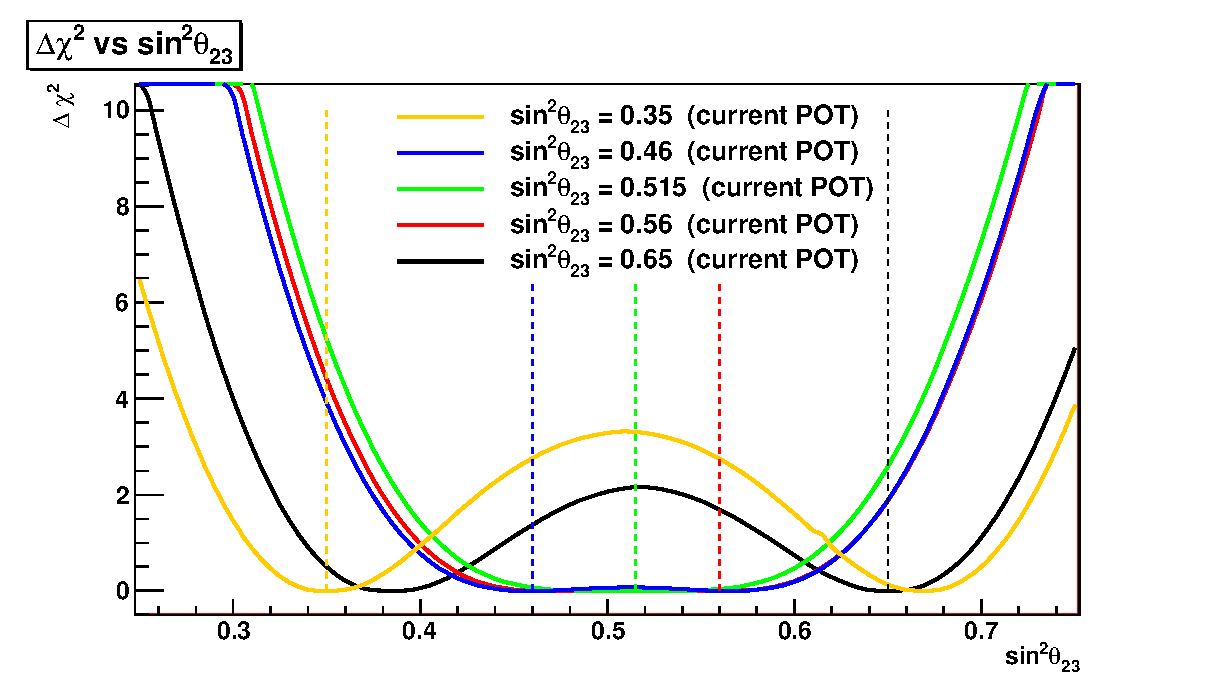
\includegraphics[width=0.5\textwidth]{images/validation/DeltaChisqVsTheta23CurrentSets.eps}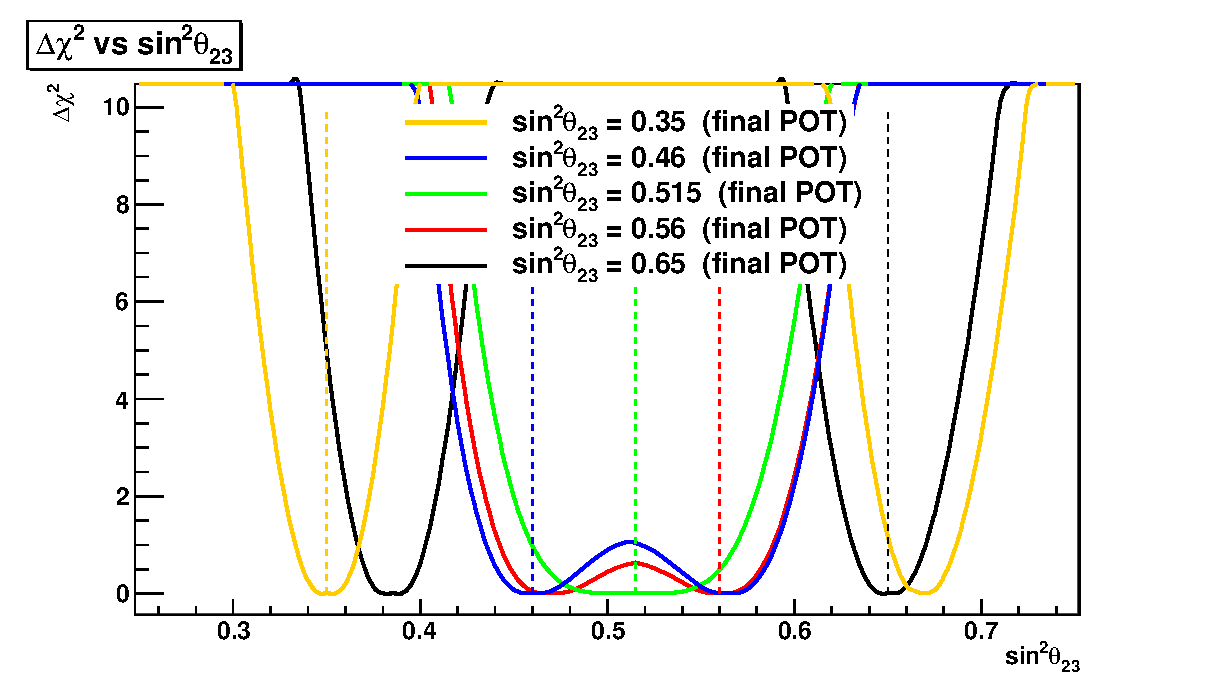
\includegraphics[width=0.5\textwidth]{images/validation/DeltaChisqVsTheta23Mock100Sets.eps}
\caption{ 1D marginalized $\Delta\chi^{2}$ distribution vs $sin^{2}\theta_{23}$ for different true input values at current POT (left) and estimated final POT (right).}
\label{fig:1Dchisqtheta23}
\end{center}
\end{figure}

 \begin{figure}[htbp]
\begin{center}
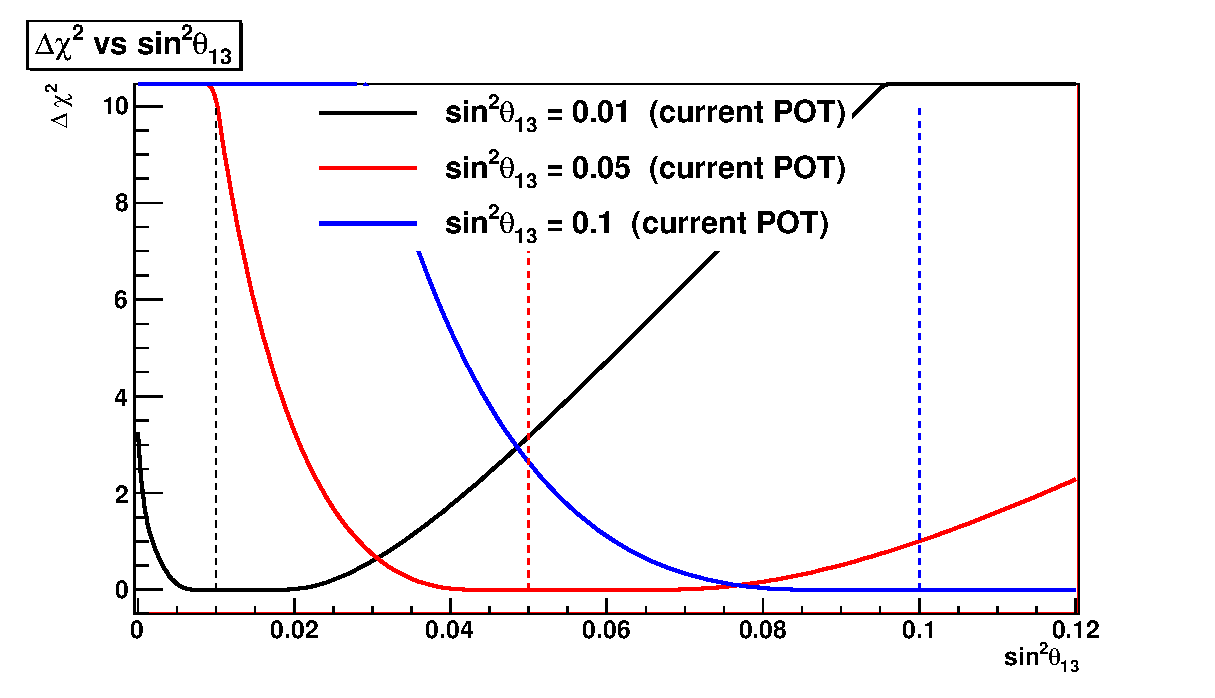
\includegraphics[width=0.5\textwidth]{images/validation/DeltaChisqVsTheta13CurrentSets.eps}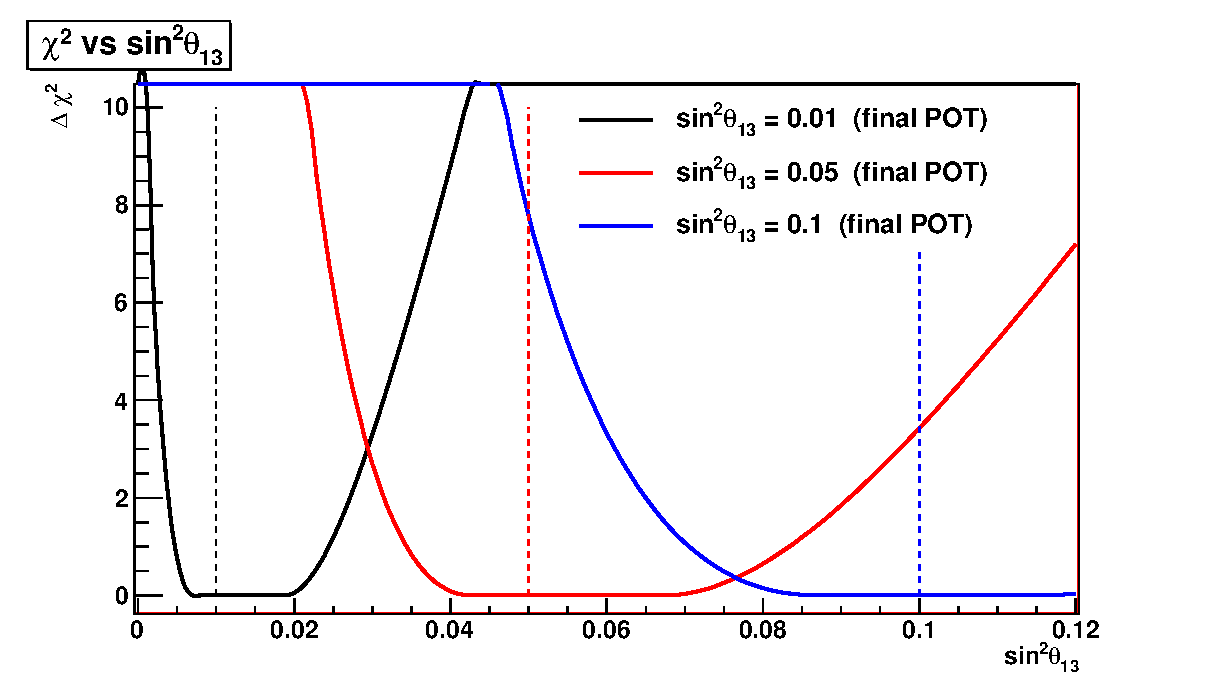
\includegraphics[width=0.5\textwidth]{images/validation/DeltaChisqVsTheta13Mock100Sets.eps}
\caption{ 1D marginalized $\Delta\chi^{2}$ distribution vs $sin^{2}\theta_{13}$ for different true input values at current POT (left) and estimated final POT (right).}
\label{fig:1Dchisqtheta13}
\end{center}
\end{figure}

 \begin{figure}[htbp]
\begin{center}
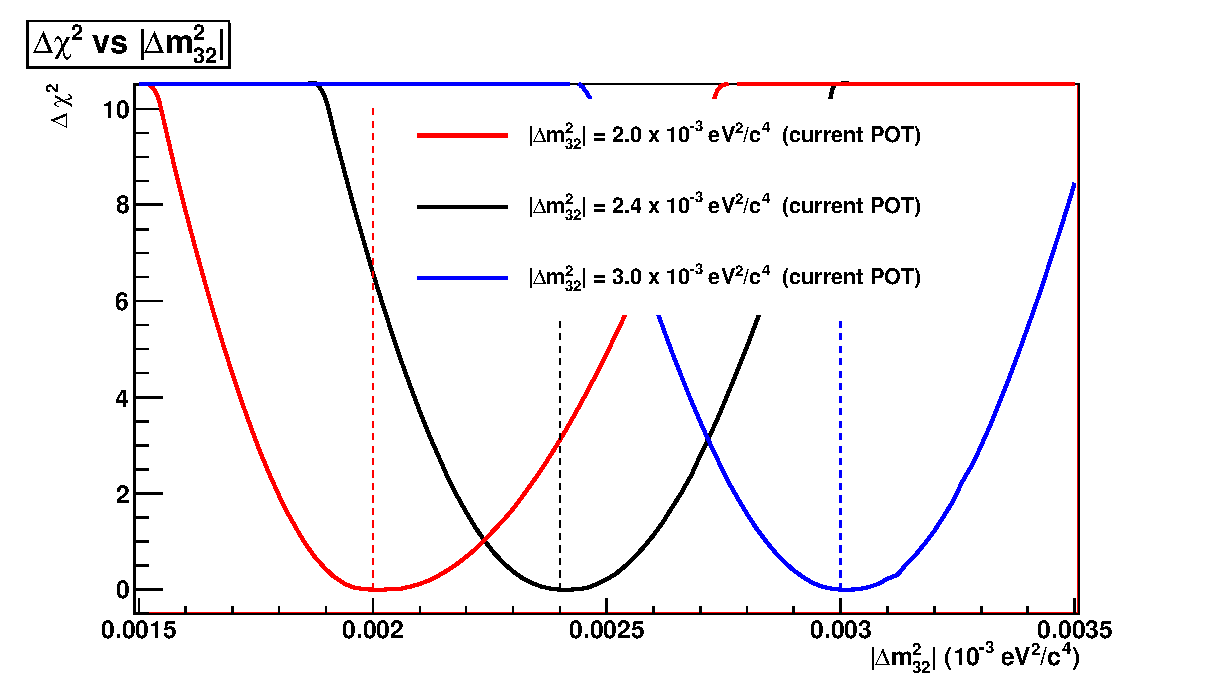
\includegraphics[width=0.5\textwidth]{images/validation/DeltaChisqVsDm23sqCurrentSets.eps}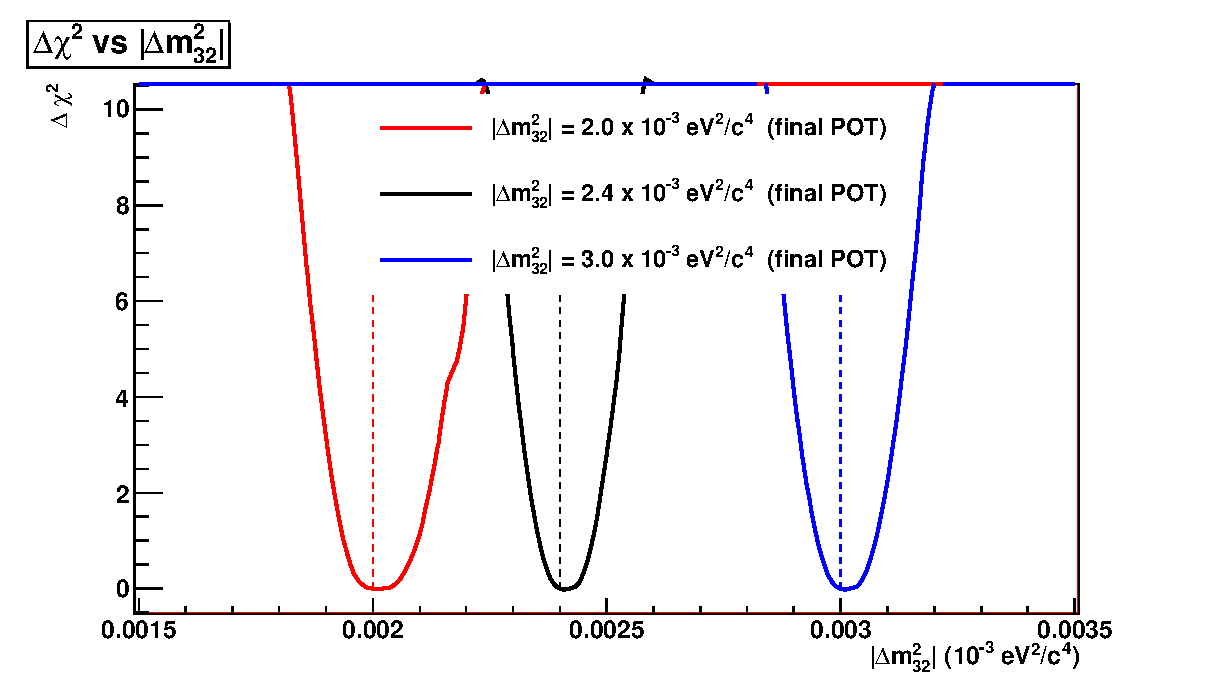
\includegraphics[width=0.5\textwidth]{images/validation/DeltaChisqVsDm23sq100Sets.eps}
\caption{ 1D marginalized $\Delta\chi^{2}$ distribution vs $\Delta m_{32}^{2}$ for different true input values at current POT (left) and estimated final POT (right).}
\label{fig:1Dchisqdm23sq}
\end{center}
\end{figure}

 \begin{figure}[htbp]
\begin{center}
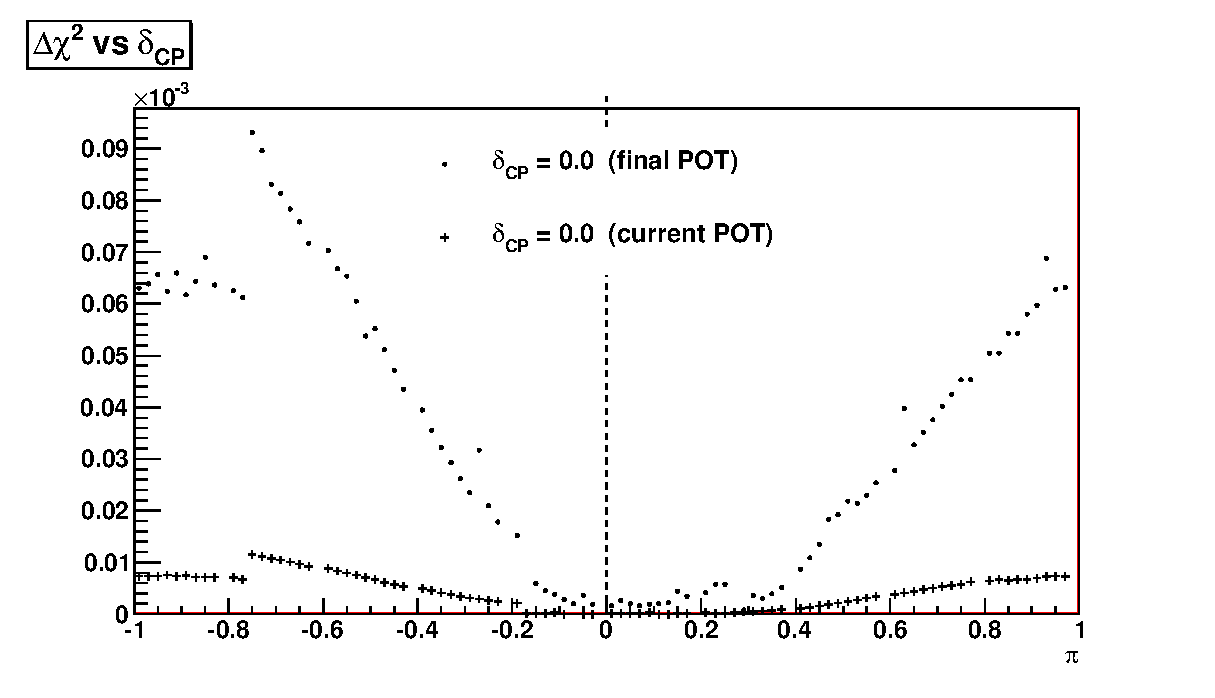
\includegraphics[width=0.5\textwidth]{images/validation/DeltaChisqVsDeltaCPSet0.eps}
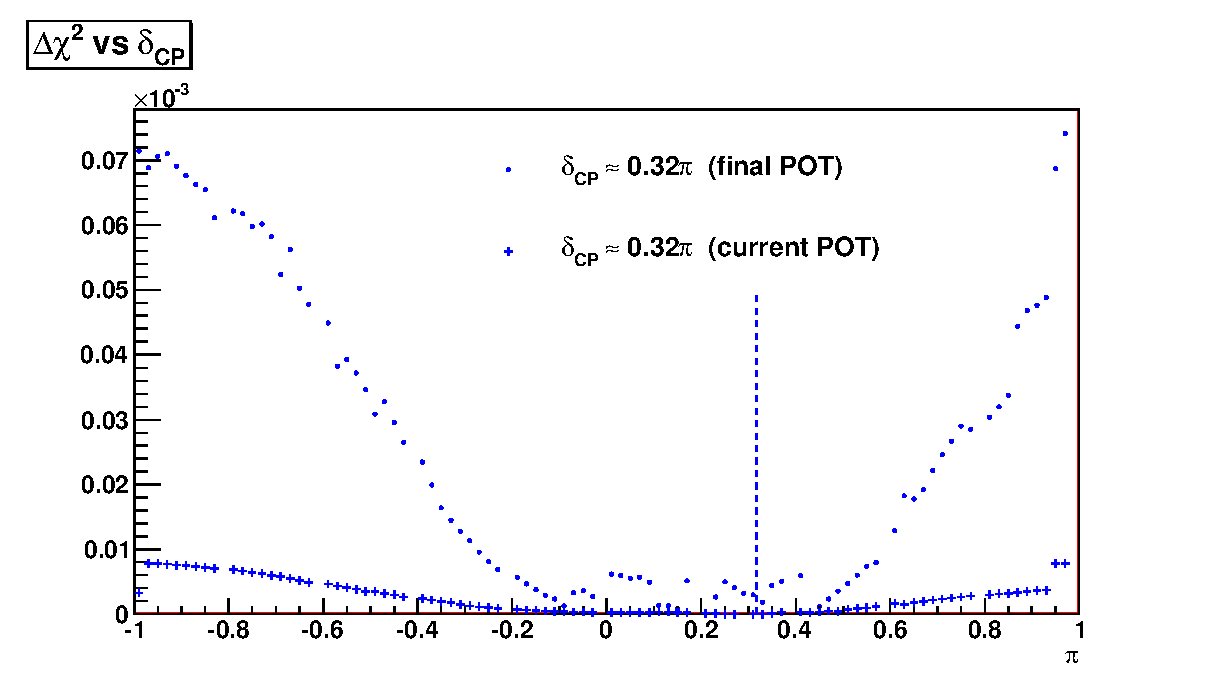
\includegraphics[width=0.5\textwidth]{images/validation/DeltaChisqVsDeltaCPSet1.eps}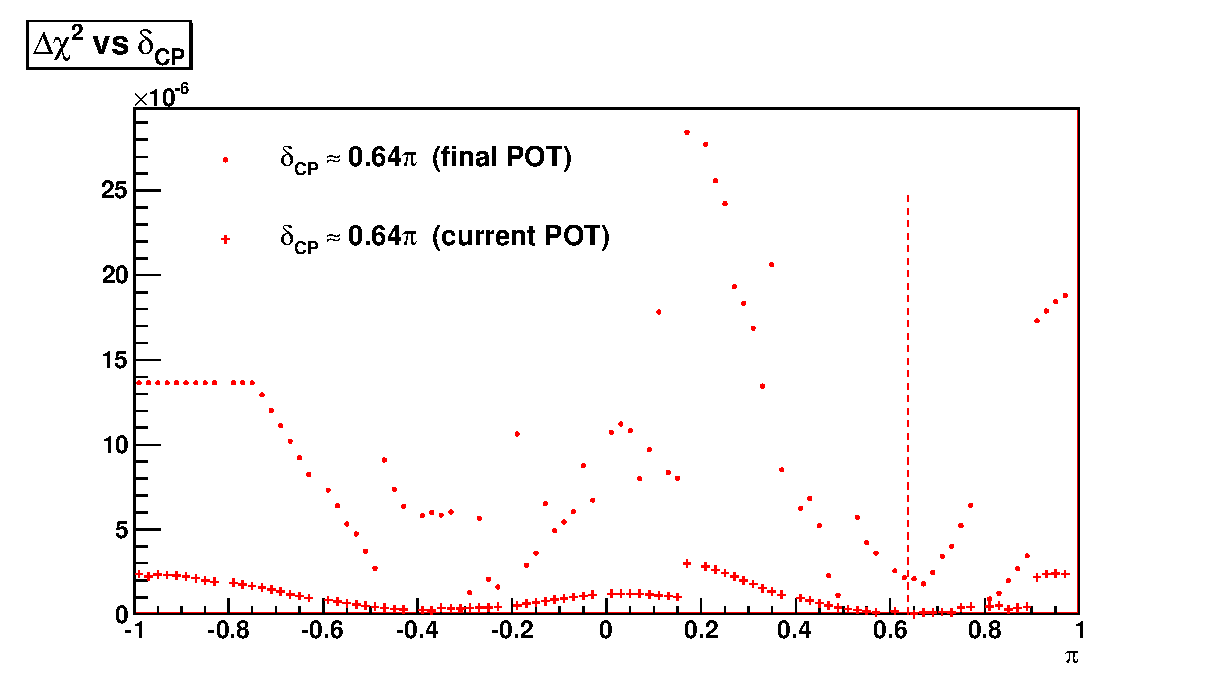
\includegraphics[width=0.5\textwidth]{images/validation/DeltaChisqVsDeltaCPSet2.eps}
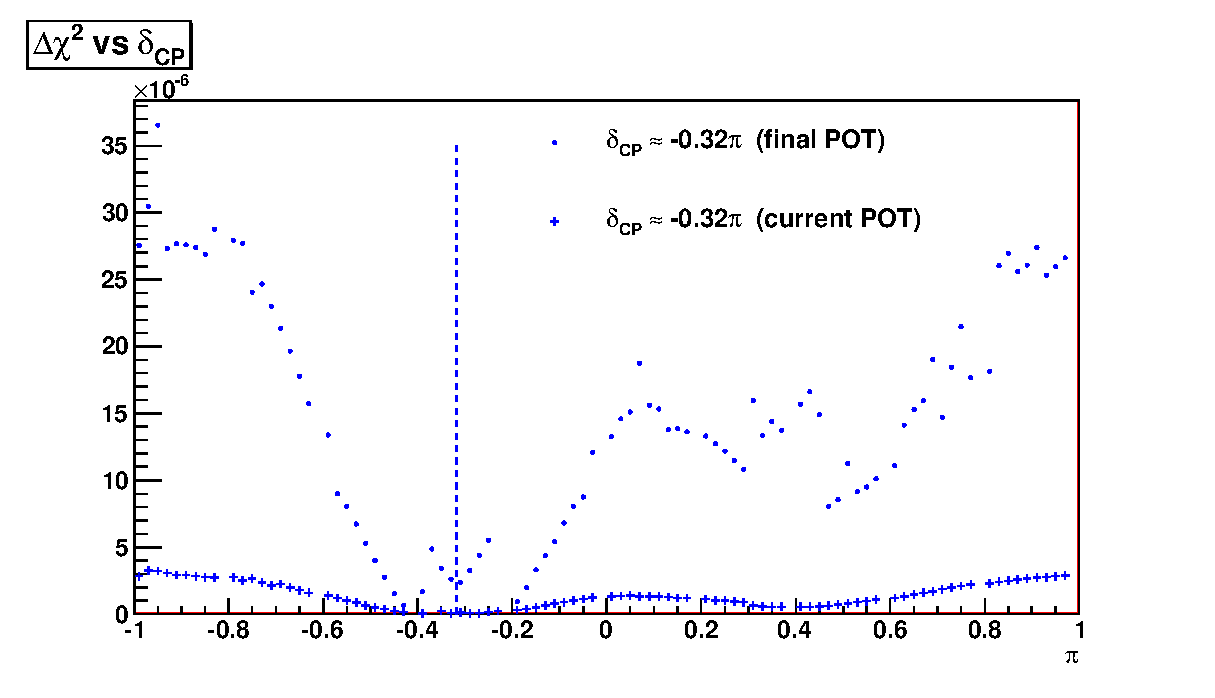
\includegraphics[width=0.5\textwidth]{images/validation/DeltaChisqVsDeltaCPSet3.eps}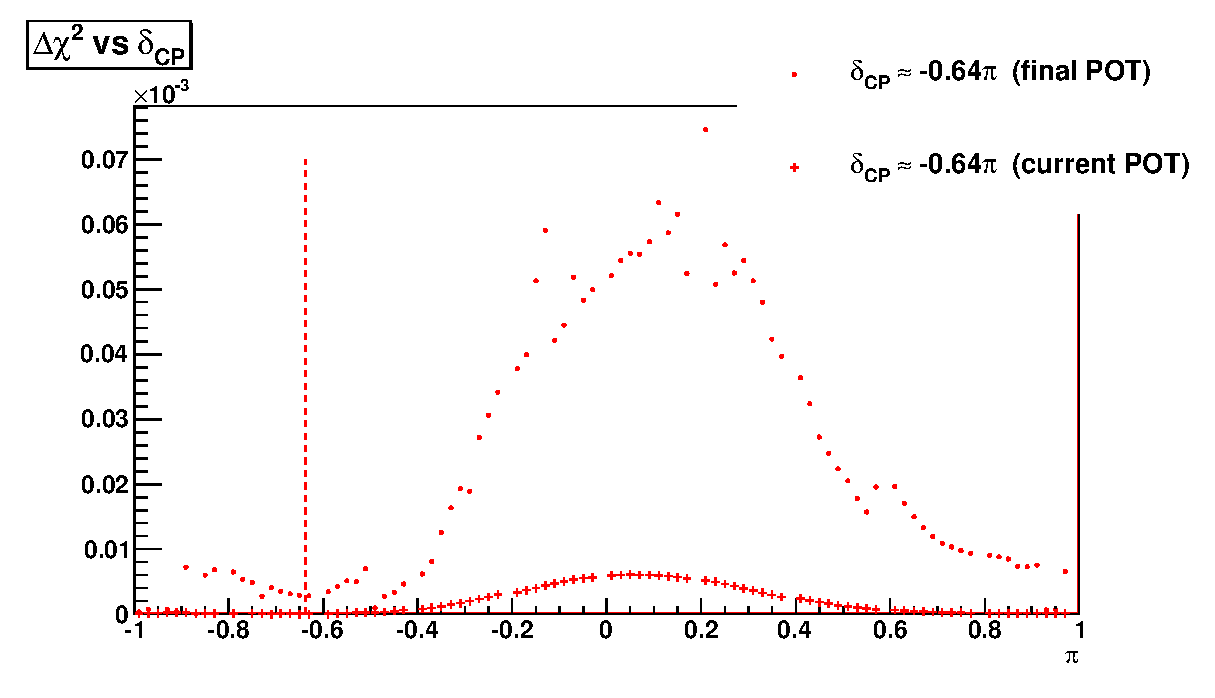
\includegraphics[width=0.5\textwidth]{images/validation/DeltaChisqVsDeltaCPSet4.eps}
\caption{ 1D marginalized $\Delta\chi^{2}$ distribution vs $\delta_{CP}$ for different true input values each one in a different plot at current POT and estimated final POT compared in each plot.}
\label{fig:1Dchisqdeltacp}
\end{center}
\end{figure}

\ \ \\


Now contours for the 68\% and 90\% confidence regions in 2D for the joint oscillation analysis are presented in two possible phase-spaces: the appearance and disappearance ones. No statistical fluctuations are allowed as they would mean different input values between grid points. In figure \ref{fig:jointapp} the contours for the joint oscillation analysis in the phase space $sin^{2}2\theta_{13}$-$\delta_{CP}$ are presented along with the fitted value of the other two oscillation parameters ($sin^{2}2\theta_{23}$, $\Delta m_{32}^{2}$) in figure \ref{fig:jointappfitted}. Figure \ref{fig:jointdisapp} shows the contours in the phase space $sin^{2}2\theta_{23}$-$\Delta m_{32}^{2}$ for the joint oscillation analysis, presented along with the fitted value of the other two oscillation parameters ($\delta_{CP}$,$sin^{2}2\theta_{13}$) in figure \ref{fig:jointdisappfitted}.


 \begin{figure}[htbp]
\begin{center}
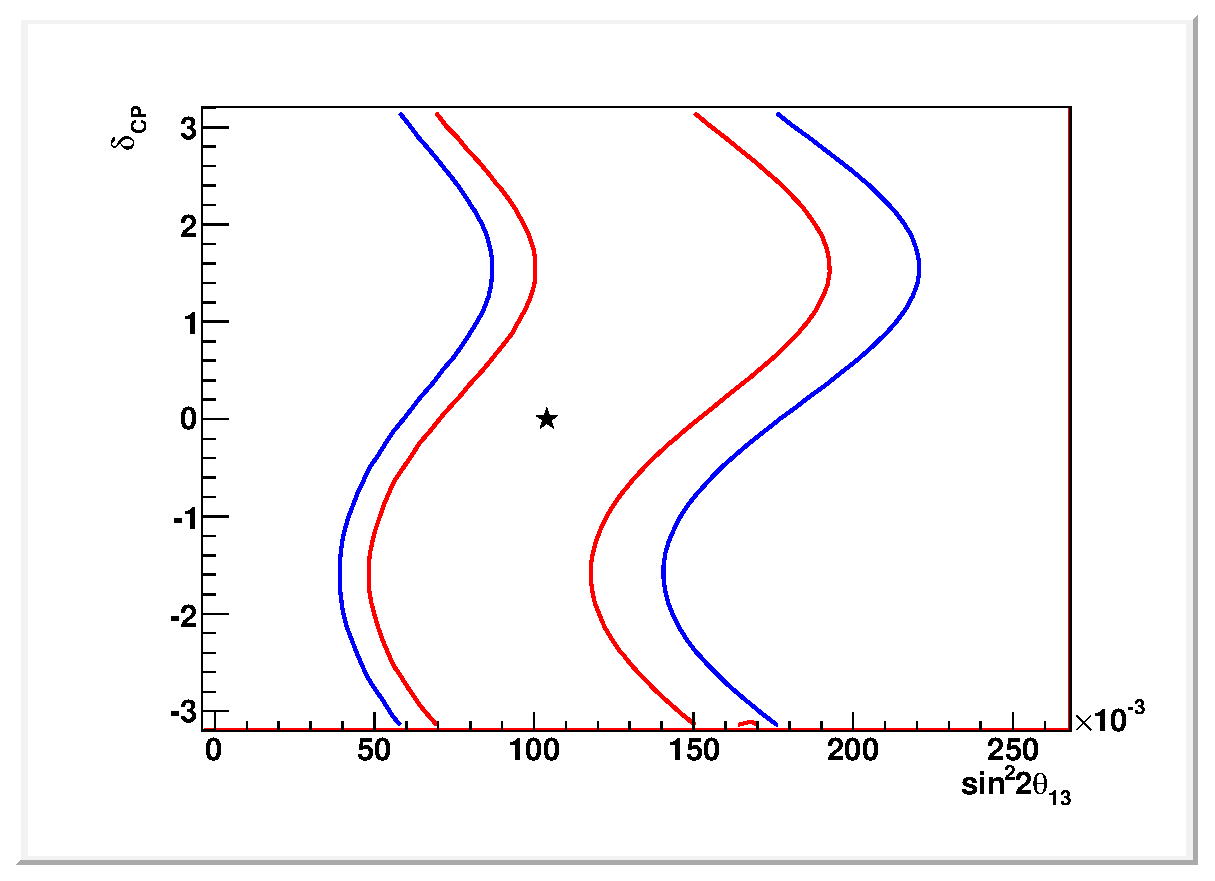
\includegraphics[width=0.7\textwidth]{images/validation/AppContoursJointOAMock100New.eps}
\caption{ 2D confidence regions of the joint oscillation analysis in the phase space $sin^{2}2\theta_{13}$-$\delta_{CP}$ for the estimated final POT.}
\label{fig:jointapp}
\end{center}
\end{figure}


 \begin{figure}[htbp]
\begin{center}
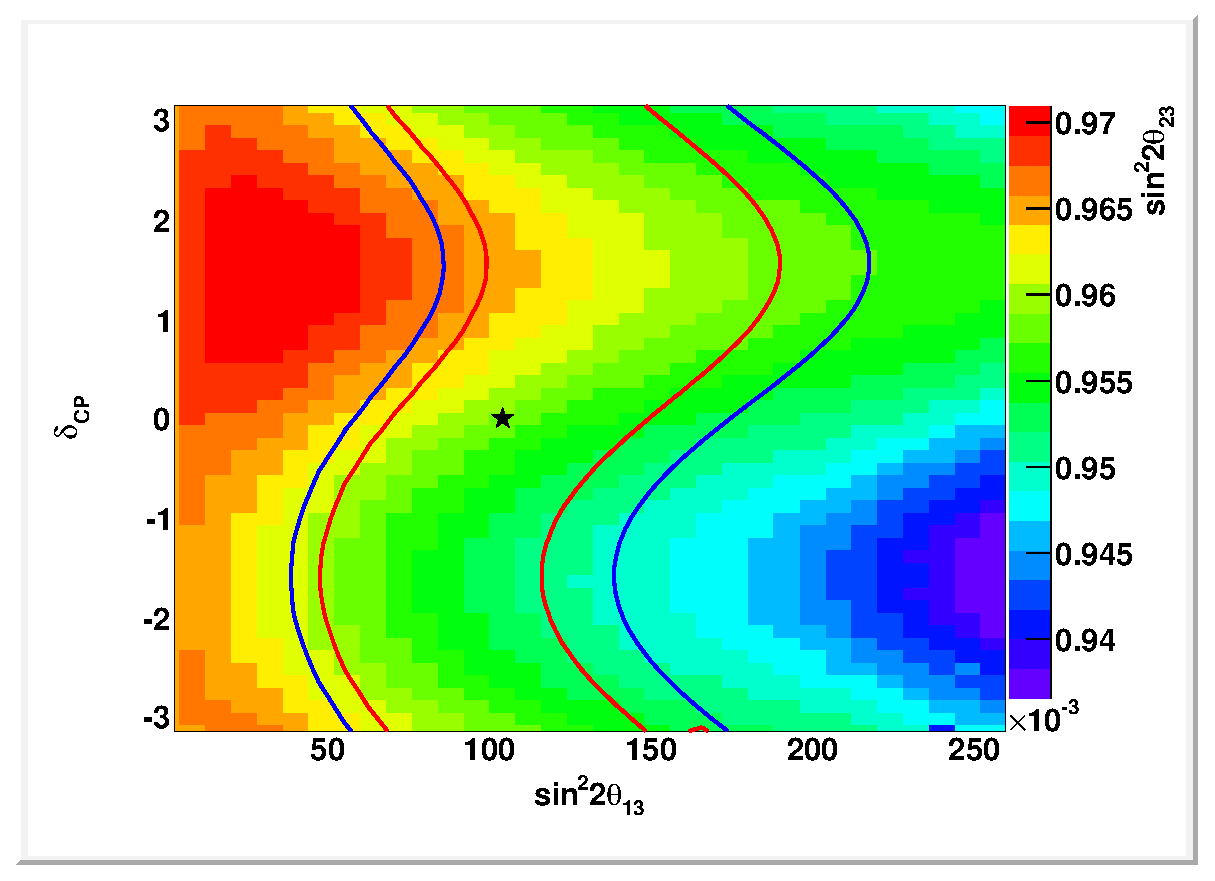
\includegraphics[width=0.5\textwidth]{images/validation/FittedTheta23JointFit.eps}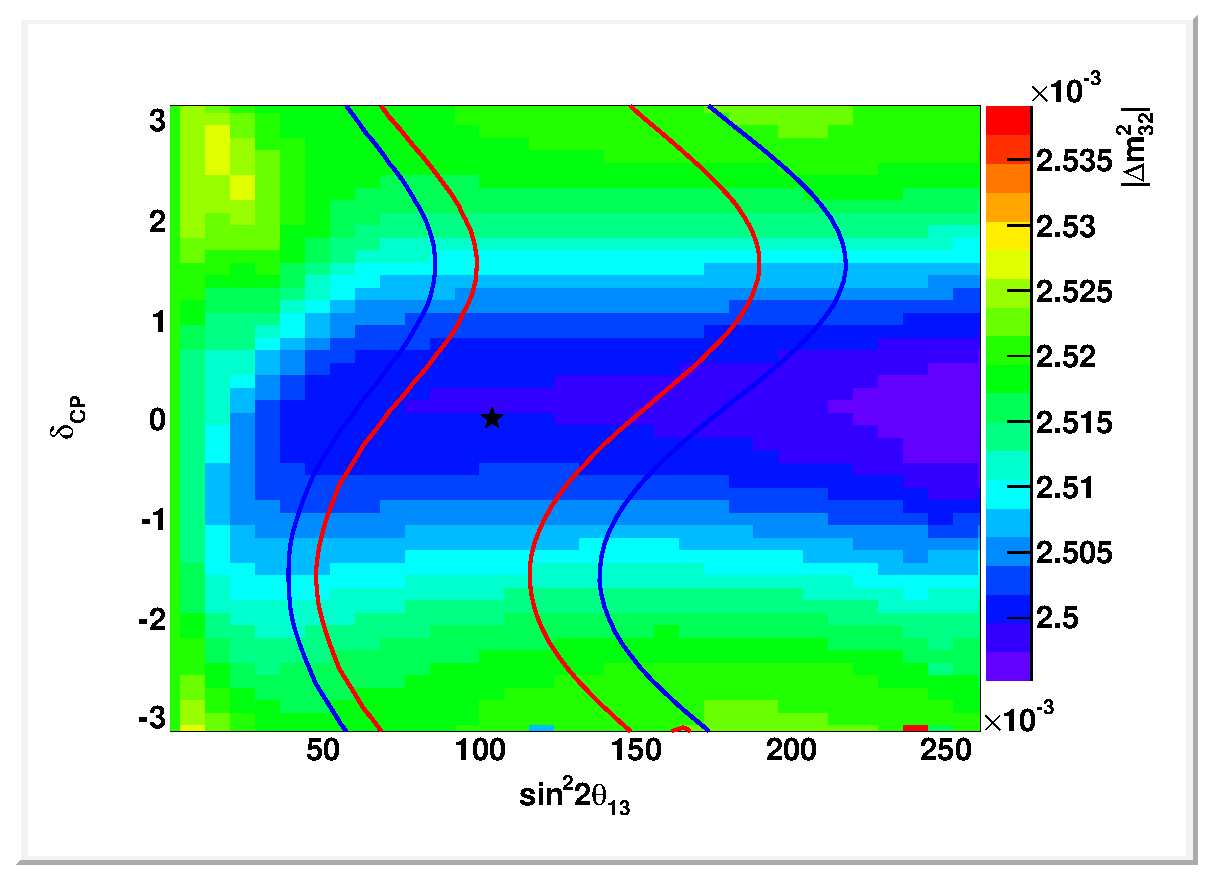
\includegraphics[width=0.5\textwidth]{images/validation/FittedDm23sqJointFit.eps}
\caption{ Fitted value of the two oscillation parameters $sin^{2}2\theta_{23}$ (left) and  $\Delta m_{32}^{2}$ (right) for the joint oscillation analysis in the phase space $sin^{2}2\theta_{13}$-$\delta_{CP}$  for the estimated final POT (contours are kept as reference).}
\label{fig:jointappfitted}
\end{center}
\end{figure}


 \begin{figure}[htbp]
\begin{center}
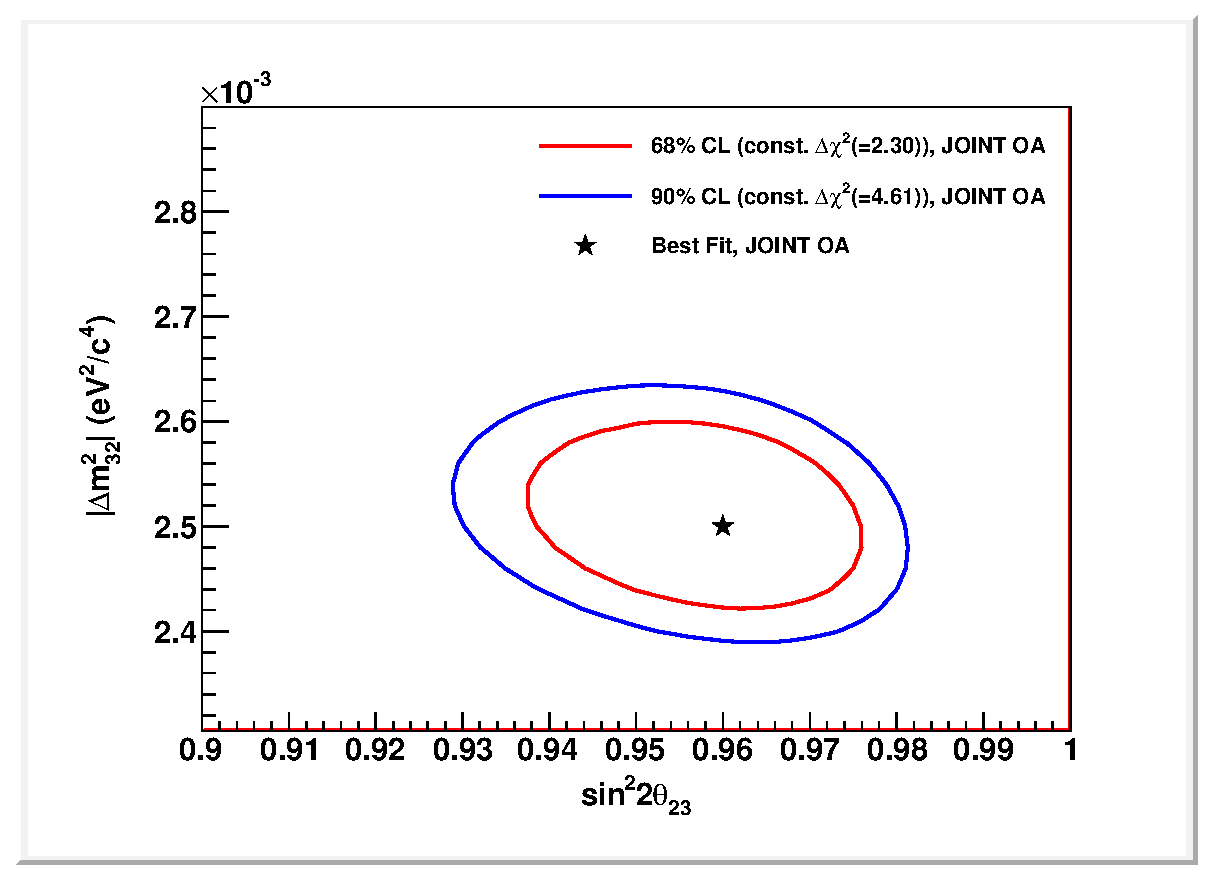
\includegraphics[width=0.7\textwidth]{images/validation/DisappContoursJointOAMock100New.eps}
\caption{ 2D confidence regions of the joint oscillation analysis in the phase space $sin^{2}2\theta_{23}$-$\Delta m_{32}^{2}$ for the estimated final POT. }
\label{fig:jointdisapp}
\end{center}
\end{figure}

 \begin{figure}[htbp]
\begin{center}
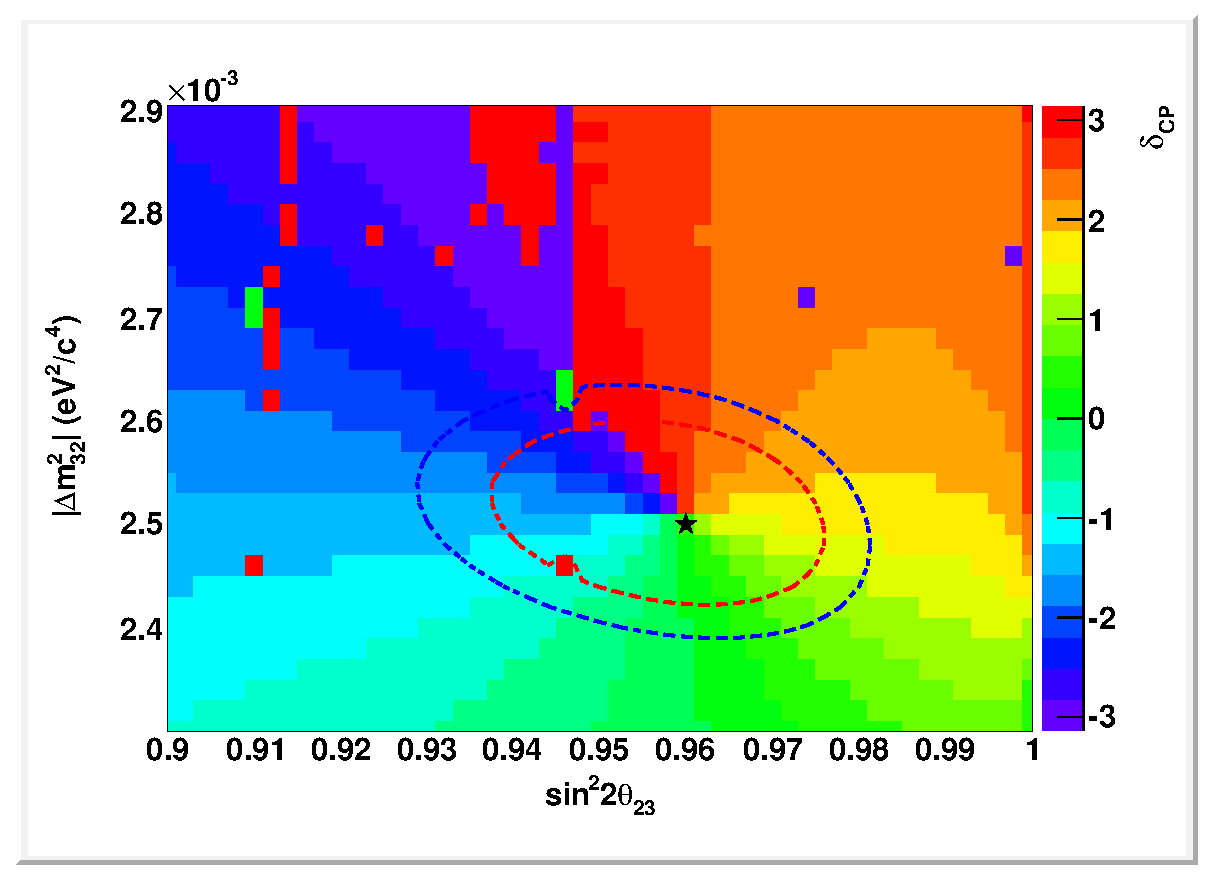
\includegraphics[width=0.5\textwidth]{images/validation/FittedDeltaCPJointFit.eps}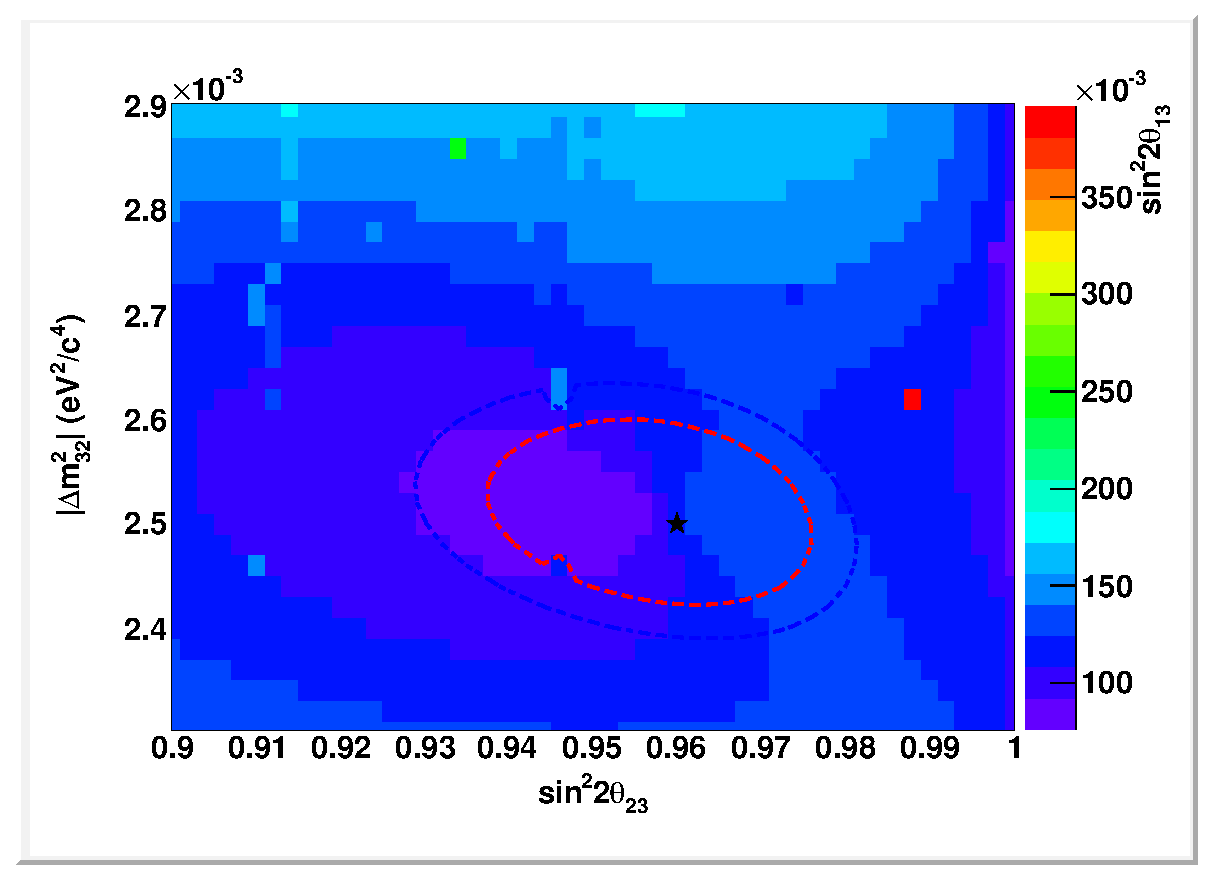
\includegraphics[width=0.5\textwidth]{images/validation/FittedTheta13JointFit.eps}
\caption{ Fitted value of the two oscillation parameters $\delta_{CP}$ (left) and $sin^{2}2\theta_{13}$ (right) for the joint oscillation analysis in the phase space $sin^{2}2\theta_{23}$-$\Delta m_{32}^{2}$ for the estimated final POT (contours are kept as reference). Several spurious points appear. }
\label{fig:jointdisappfitted}
\end{center}
\end{figure}

Table \ref{tab:jointOAbestfit} shows a comparison of the true oscillation parameters used to create the toy MC experiment and the best fit point result of the joint oscillation fit in the two configurations (appearance in middle row and disappearance in bottom row). The value of the two oscillation parameters scanned is taken as the central value of the grid point where the best fit point was found, for the other two hidden oscillation parameters the value presented is the fitted value of the hidden parameter at the best fit point.

\begin{table}[h]
\centering
\begin{tabular}{|c|c|c|c|c|}
\hline
  & $sin^{2}2\theta_{23}$ & $\Delta m_{32}^{2} (10^{-3} eV^{2}/c^{4})$  & $sin^{2}2\theta_{13}$ & $\delta_{CP}$ \\
\hline \hline
{\color{blue}{Toy MC experiment}} & {\color{blue}{0.96}} & {\color{blue}{2.5}} & {\color{blue}{0.12}} & {\color{blue}{0.5}} \\
Joint OA: Best fit point (appearance configuration) &  0.958& 2.499& 0.104 &  0\\
Joint OA: Best fit point (disappearance configuration) & 0.96 & 2.5 & 0.12003 & 0.501\\
\hline
\end{tabular}
\caption{ Comparison of the true oscillation parameters used to create the toy MC experiment and the best fit point result of the joint oscillation fit in the two configurations (appearance in middle row and disappearance in bottom row). }
\label{tab:jointOAbestfit}
\end{table}

From the results in figures \ref{fig:jointapp} and \ref{fig:jointdisapp} and table \ref{tab:jointOAbestfit} it is clear the good recovery of the true input values by the joint oscillation analysis at its best fit point. In the appearance configuration the global best fit point appears at $\delta_{CP}=0$, a further study revealed that the second minimum of $\chi^{2}$ appears at $\delta_{CP}=0.5, sin^{2}2\theta_{13}=0.12$, exactly the true input value, and the difference in $\chi^{2}$ between those first and second best fit points is of  $1\times10^{-5}$. On the other hand, the size of the confidence regions in figures \ref{fig:jointapp} and \ref{fig:jointdisapp} gives a first idea of how the final contours (at final expected POT) will look like, with the caveat that the systematic errors used are as 2010 analysis, so the size of the confidence regions would decrease a little with realistic systematics at the end of the T2K running time. 

\subsubsection{Compare sensitivity plots for the joint oscillation analysis vs stand-alone analyses}

For comparison purposes, several stand-alone analyses are performed for this work. Unless otherwise specified, the method will be the same as for the joint fit, i.e. contours will be created fitting for systematic parameters (along with some oscillation parameters if the study requires it), and built using the constant $\Delta\chi^{2}$ method explained. But it is to keep in mind that the stand-alone analyses differ from the joint fit in the fact that they only use one sample in the computation of $\chi^{2}$. So for the stand-alone $\nu_{\mu}$-disappearance ($\nu_{e}$-appearance) analysis performed in this work, contours are built marginalizing $\chi^{2}=\chi^{2}_{\mu}+\chi^{2}_{penalty;syst}$ ($\chi^{2}=\chi^{2}_{e}+\chi^{2}_{penalty;syst}$). In illustration cases, some oscillation parameters are included in the fit also for the stand-alone analyses. For instance, it will be presented a stand-alone $\nu_{\mu}$-disappearance analysis fitting also for $sin^{2}2\theta_{13}$ and $\delta_{CP}$. Such study was done to see the effect of adding two extra parameters in the fit, and the impossibility for the fitter to deal with the appearance parameters without the appropriate sample, because, and this is the idea to be highlighted, even if other oscillation parameters are included for the fit, such as $sin^{2}2\theta_{13}$ and $\delta_{CP}$, the stand-alone analysis ($\nu_{\mu}$-disappearance analysis in this case) is only using the $1R_{\mu}$ sample, versus the joint fit, which is combining always both $1R_{\mu}$ and $1R_{e}$ samples. Moreover, the list of systematic uncertainties will be slightly different, being removed in each case the uncertainties only related to the missing sample. 

{\color{red}{TO INCLUDE: Comparison of 1D $\Delta\chi^{2}$ for joint vs standalone. Worked on this today but need to check }}

There are several ways the results for the 2D contours plots for the joint analysis and the stand-alone ones can be compared. First of all a process in two steps with the parallel stand-alone analyses will be done in order to imitate as good as possible the usual mechanic of the stand-alone analyses. The true input values for the toy MC experiment in any of these tests are common and were already presented in table \ref{tab:jointOAbestfit}

\renewcommand{\labelitemi}{$\bullet$} 

\labelitemi{ \textbf{Step I : Stand-alone appearance analysis fixing $sin^{2}2\theta_{23}$ to maximal.}}
As we have already mentioned in section \ref{sec:motivation}, usually the stand-alone appearance analysis assumes maximal $sin^{2}2\theta_{23}=1.0$ as prior. Figure \ref{fig:appstand} shows the result of the stand-alone appearance analysis fitting the toy MC experiment fixing $sin^{2}2\theta_{23}$ to maximal (light colors, solid lines) compared with the result of the same stand-alone appearance analysis fixing $sin^{2}2\theta_{23}$ to the true input value, $sin^{2}2\theta_{23}$=0.96, (dark colors, dashed lines). Clearly there is a bias between both confidence regions and best fit points. Comparing now the contours created with the joint oscillation analysis (dark colors, solid lines) and the stand-alone appearance analysis fixing $sin^{2}2\theta_{23}$ to the true input value in figure \ref{fig:appstandjoint}, there is no bias between them. It will be assumed that in reality the stand-alone appearance analysis is done fixing $sin^{2}2\theta_{23}$ to maximal and therefore the values of the best fit point found for that analysis will be the ones used in next step. Also, as it is done in the actual process, the best fit point used will be at value $\delta_{CP}=0$; in this case at $\delta_{CP}=0$, $sin^{2}2\theta_{13}=0.08$. 

 \begin{figure}[htbp]
\begin{center}
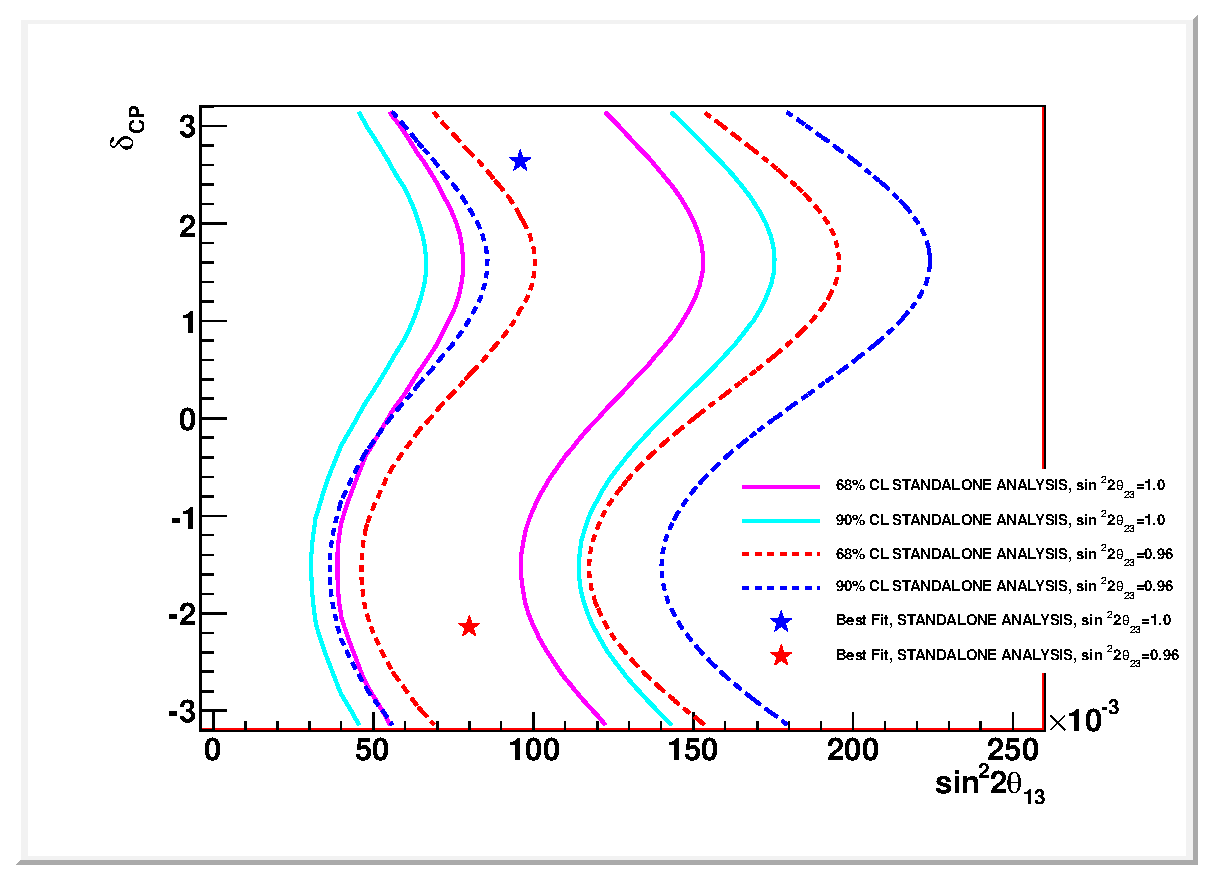
\includegraphics[width=0.7\textwidth]{images/validation/AppContoursMock100FixedVsFixedTrue.eps}
\caption{ 2D confidence regions in the phase space $sin^{2}2\theta_{13}$-$\delta_{CP}$ for the stand-alone appearance analysis fixing $sin^{2}2\theta_{23}$ to maximal (light colors, solid lines) and fixing $sin^{2}2\theta_{23}$ to the true input value, $sin^{2}2\theta_{23}$=0.96, (dark colors, dashed lines) for the estimated final POT.}
\label{fig:appstand}
\end{center}
\end{figure}

 \begin{figure}[htbp]
\begin{center}
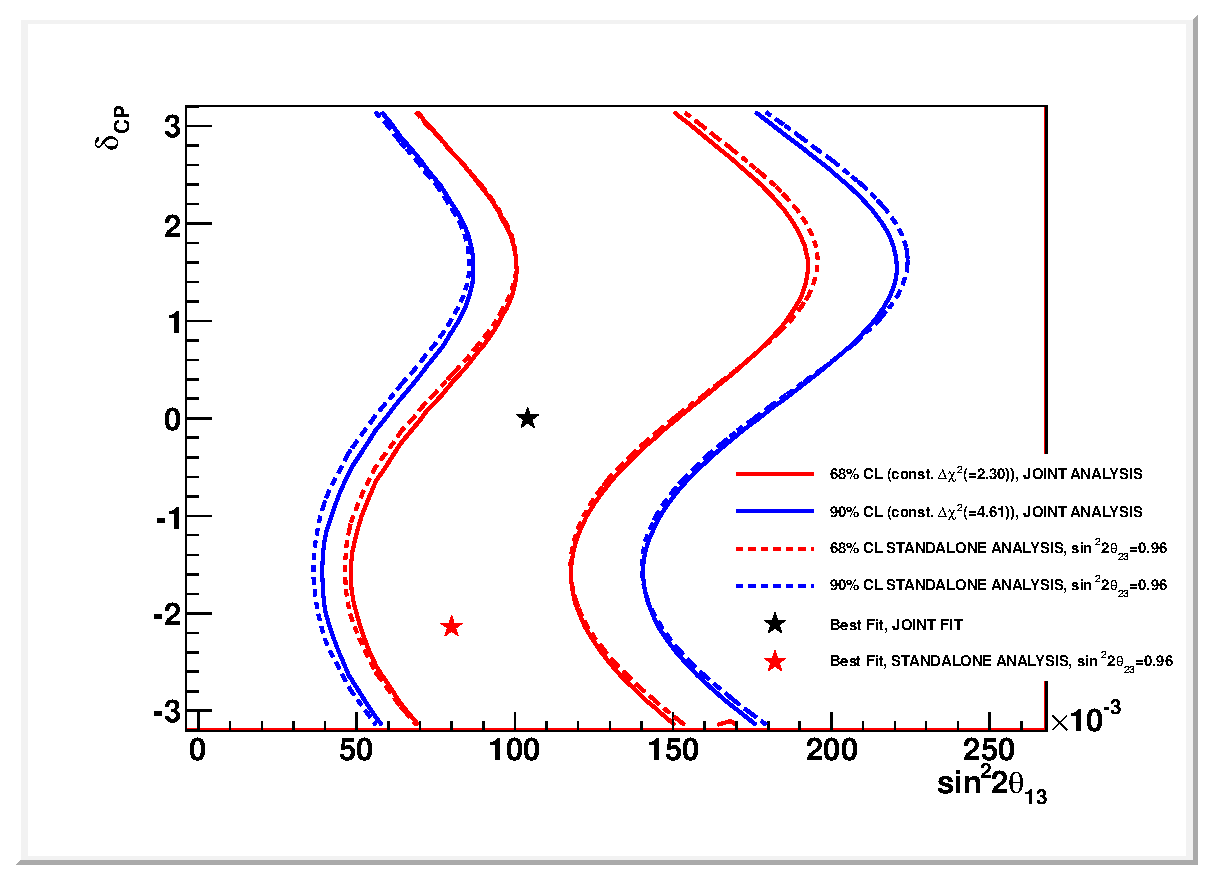
\includegraphics[width=0.7\textwidth]{images/validation/AppContoursJointOAMock100NewVsFixedTrue.eps}
\caption{Comparison of 2D confidence regions in the phase space $sin^{2}2\theta_{13}$-$\delta_{CP}$ for the stand-alone appearance analysis fixing $sin^{2}2\theta_{23}$ to the true input value, $sin^{2}2\theta_{23}$=0.96, (dark colors, dashed lines) and the ones obtained using the joint oscillation analysis (dark colors, solid lines) for the estimated final POT.}
\label{fig:appstandjoint}
\end{center}
\end{figure}

\labelitemi{ \textbf{Step II : Stand-alone disappearance analysis using the result from step I to fix the other oscillation parameters. }}
Now imagine the disappearance analysis is done using as priors the best results available, so the latest result for the appearance analysis carried out in step I. Then, for the disappearance analysis now, the priors for the other two oscillation parameters will be $\delta_{CP}=0$, $sin^{2}2\theta_{13}=0.08$. Figure \ref{fig:disappstandjoint} shows the comparison between the result obtained for the stand-alone disappearance analysis built with those premises (dashed lines) and the joint oscillation analysis (solid lines). There is a bias between the best fit points and a rotation between contours as a consequence of the incorrect input values used to fixed $\delta_{CP}$ and $sin^{2}2\theta_{13}$ in the stand-alone case.

 \begin{figure}[htbp]
\begin{center}
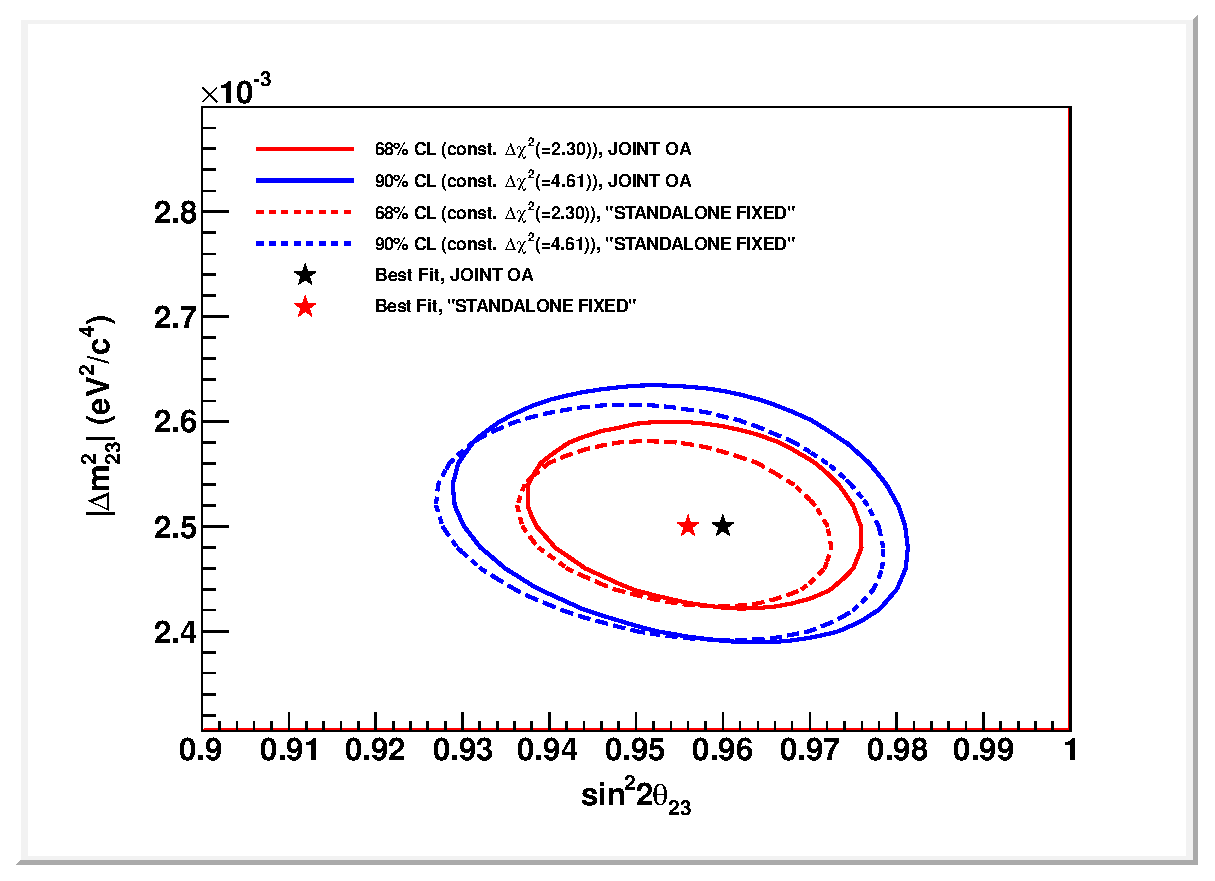
\includegraphics[width=0.7\textwidth]{images/validation/DisappContoursJointOAMock100NewVsFixed.eps}
\caption{Comparison of 2D confidence regions in the phase space $sin^{2}2\theta_{23}$-$\Delta m_{32}^{2}$ for the stand-alone appearance analysis fixing $\delta_{CP}=0$, $sin^{2}2\theta_{13}=0.08$ (from result in figure \ref{fig:appstand}, dashed lines) and the ones obtained using the joint oscillation analysis (solid lines) for the estimated final POT.}
\label{fig:disappstandjoint}
\end{center}
\end{figure}

The results shown in step I and step II mean a clear advantage of using the joint oscillation analysis instead of two parallel separated appearance and disappearance analysis. 

So far the differences observed between the joint oscillation analysis and stand-alone analyses are biases in the best fit point and therefore in the contours, and rotations of the contours as well. However, the size of the contours was comparable for the joint oscillation analysis with any of the other stand-alone analyses. The reason is that although the number of parameters to fit increases, the sample containing the corresponding information is also added in the joint analysis. To check the effect of adding more parameters to the fit but without adding the extra necessary information the following test was performed. Figure \ref{fig:disappstandfitjoint} shows the effect of performing the stand-alone disappearance analysis marginalizing also the other two oscillation parameters  $\delta_{CP}$ and $sin^{2}2\theta_{13}$. Contours are larger due to the addition of two more parameters in the fit but no more information (the necessary sample, $1R_{e}$ is not included in the stand-alone analysis, while it is in the joint analysis). 

 \begin{figure}[htbp]
\begin{center}
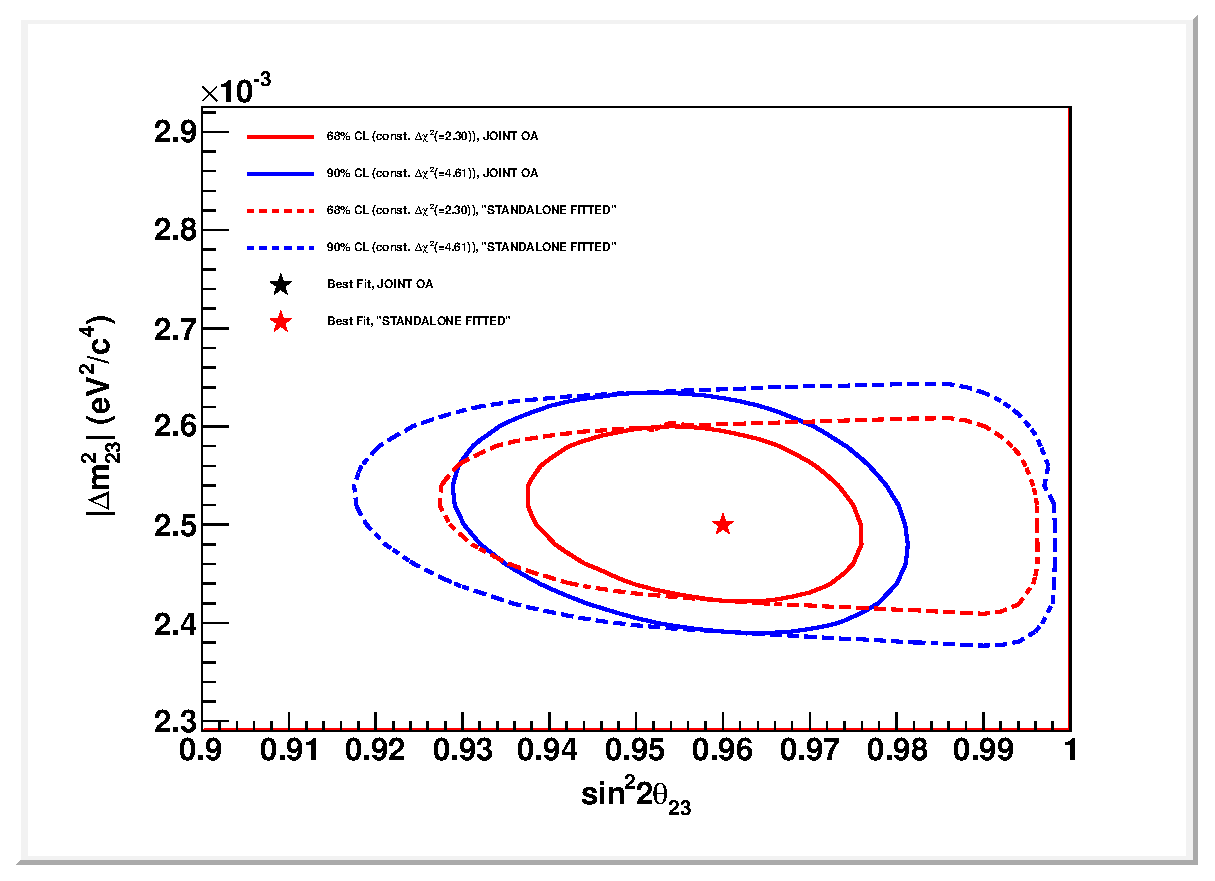
\includegraphics[width=0.7\textwidth]{images/validation/DisappContoursJointOAMock100NewVsFitted.eps}
\caption{Comparison of 2D confidence regions in the phase space $sin^{2}2\theta_{23}$-$\Delta m_{32}^{2}$ for the stand-alone appearance analysis marginalizing $\delta_{CP}$ and $sin^{2}2\theta_{13}$ (dashed lines) and the ones obtained using the joint oscillation analysis (solid lines) for the estimated final POT.}
\label{fig:disappstandfitjoint}
\end{center}
\end{figure}

The explanation for the odd shape of the contours in the stand-alone analysis marginalizing $\delta_{CP}$ and $sin^{2}2\theta_{13}$ comes in fact from the values of those parameters obtained in the fit. As presented in figure \ref{fig:disappstandfitted}, the distributions of fitted value of the parameter $sin^{2}2\theta_{13}$ tend to go to extreme values (limits in the fit) in regions in concordance with the deformation of the shape of the contours in figure \ref{fig:disappstandfitjoint}.

 \begin{figure}[htbp]
\begin{center}
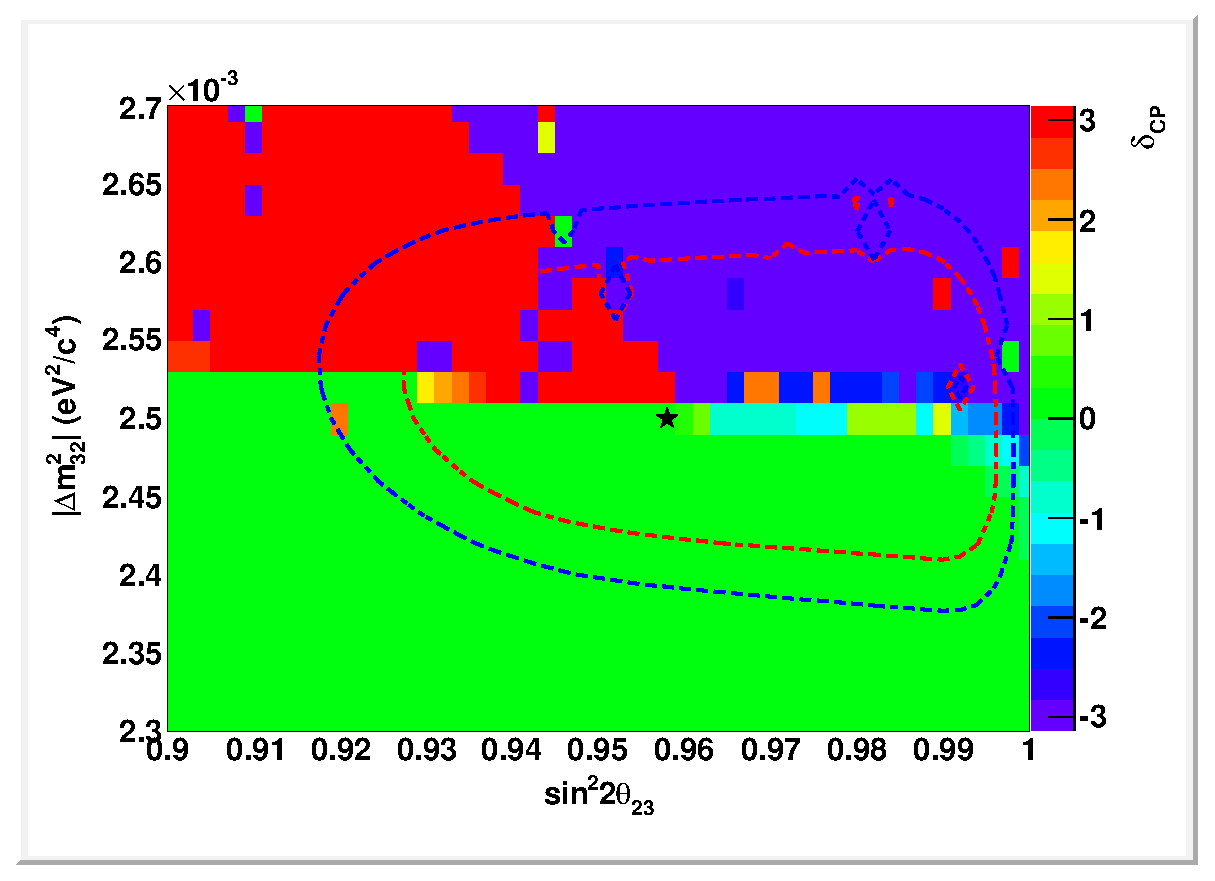
\includegraphics[width=0.5\textwidth]{images/validation/FittedDeltaCPStandFitted.eps}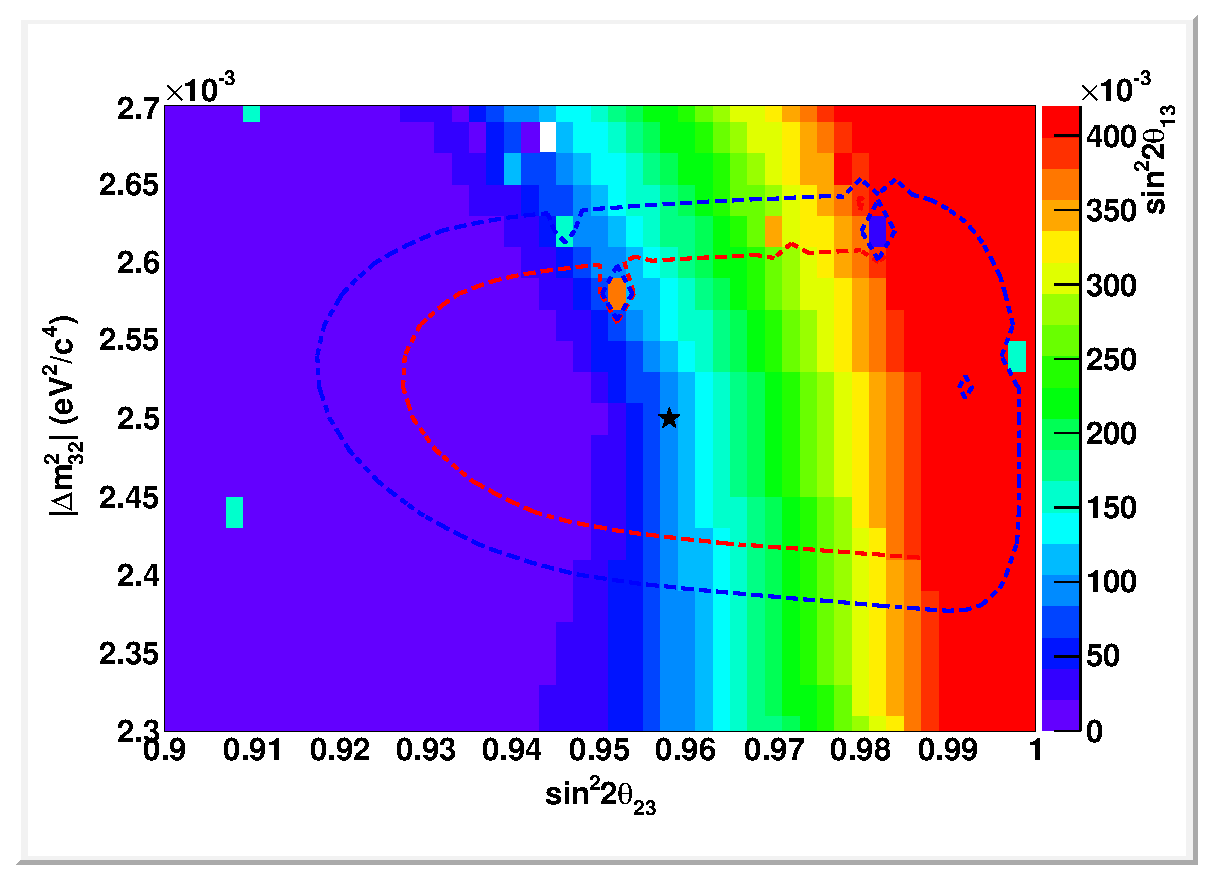
\includegraphics[width=0.5\textwidth]{images/validation/FittedTheta13PStandFitted.eps}
\caption{Fitted value of $\delta_{CP}$ (left) and $sin^{2}2\theta_{13}$ (right) for the stand-alone appearance analysis marginalizing $\delta_{CP}$ and $sin^{2}2\theta_{13}$. Several very clear spurious points appear specially for $sin^{2}2\theta_{13}$ for the estimated final POT.}
\label{fig:disappstandfitted}
\end{center}
\end{figure}

%%%%%%%%%%%%%%%%%%%%
%%%% Solar %%%%%%%%%
\subsection{Study of the effect of 12-sector parameters on the joint oscillation analysis sensitivity}
\label{sec:solar}

Another interesting study carried out is concerning the effect of the solar parameters $sin^{2}2\theta_{12}$-$\Delta m_{21}^{2}$ in the joint analysis. In the present test the solar parameters were allowed to vary so they were included in the fit and marginalized. As shown in figure \ref{fig:solar} the contours for the joint oscillation analysis became larger when the solar parameters were included in the fit. A careful check is now necessary to understand this result. When looking at figure \ref{fig:solarfit}, where the values returned by the fitter for the solar parameters are presented, it is clear that those fitted values are not correct, and the fit is just returning some extreme values of those (limits in the fit) as it already happened in the previous test (stand-alone disappearance analysis marginalizing  $\delta_{CP}$ and $sin^{2}2\theta_{13}$ ). So the conclusion is that there is no effect of the solar parameters in our samples (the fitter could not fit for those parameters, returning just the bounds of the fit) and the fact that contours became larger when marginalizing them is simply an artifact, just because more parameters were added to the fit without the necessary information. 
 
 
  \begin{figure}[htbp]
\begin{center}
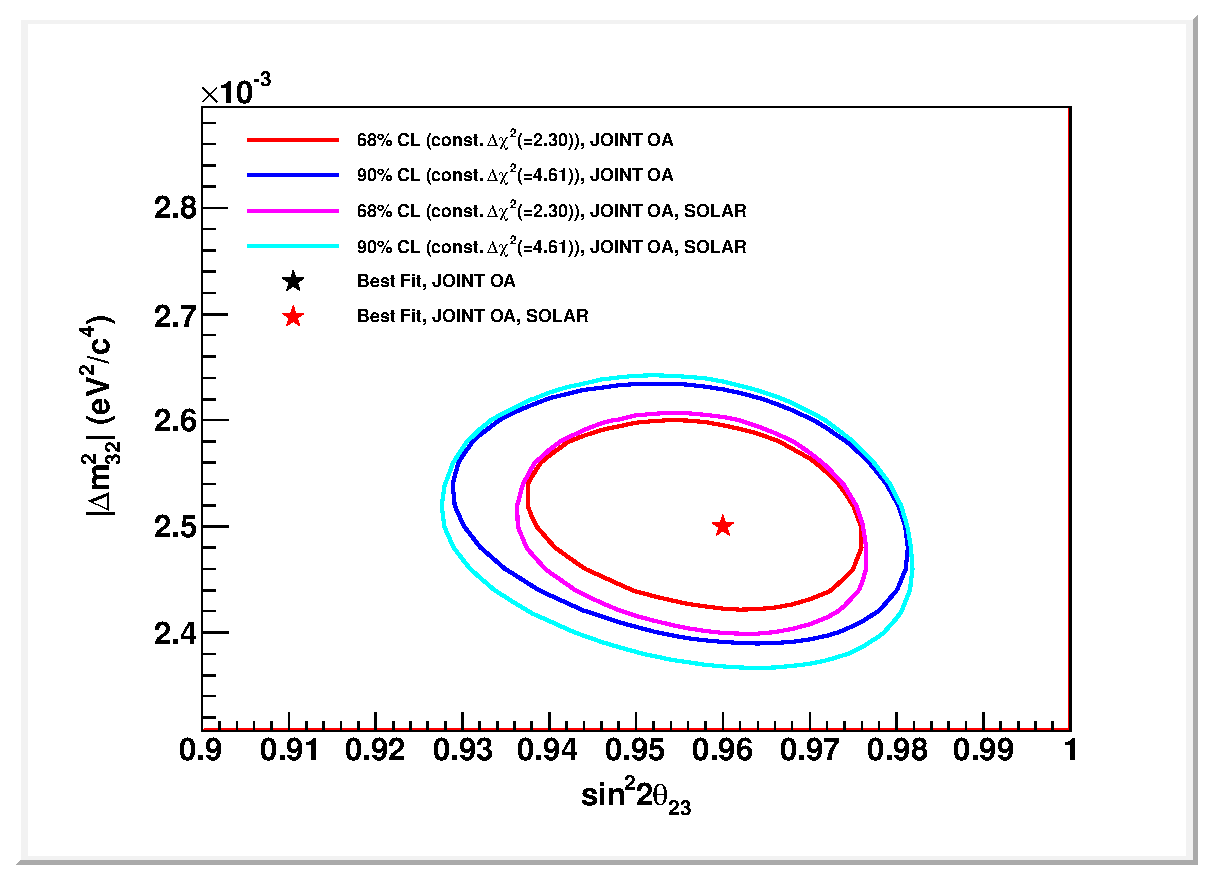
\includegraphics[width=0.7\textwidth]{images/validation/AppContoursJointOAMock100NewVsSolar.eps}
\caption{Comparison of 2D confidence regions in the phase space $sin^{2}2\theta_{23}$-$\Delta m_{32}^{2}$ for the joint oscillation analysis fixing solar parameters (dark colors, solid lines) and marginalizing them (light colors, solid lines) for the estimated final POT.}
\label{fig:solar}
\end{center}
\end{figure}


 \begin{figure}[htbp]
\begin{center}
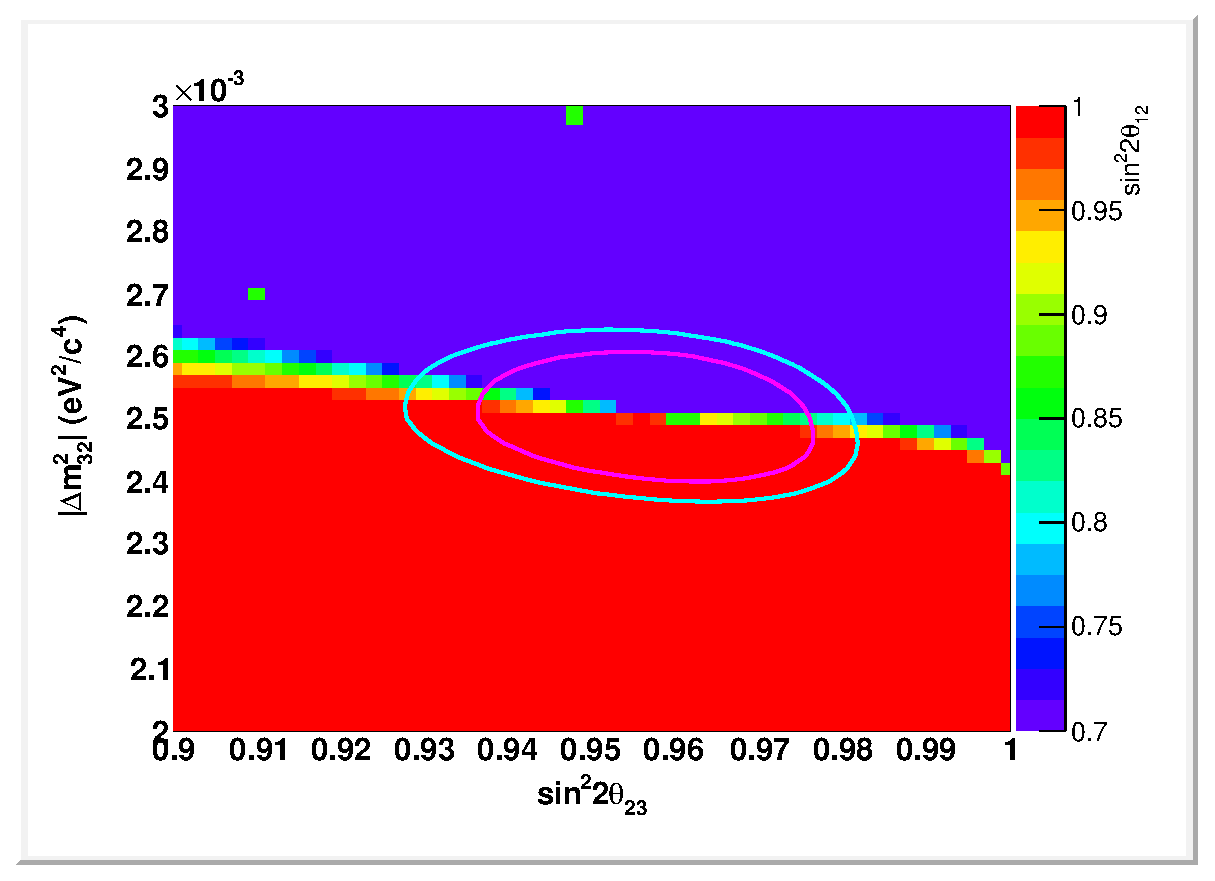
\includegraphics[width=0.5\textwidth]{images/validation/FittedTheta12JointFitSolar.eps}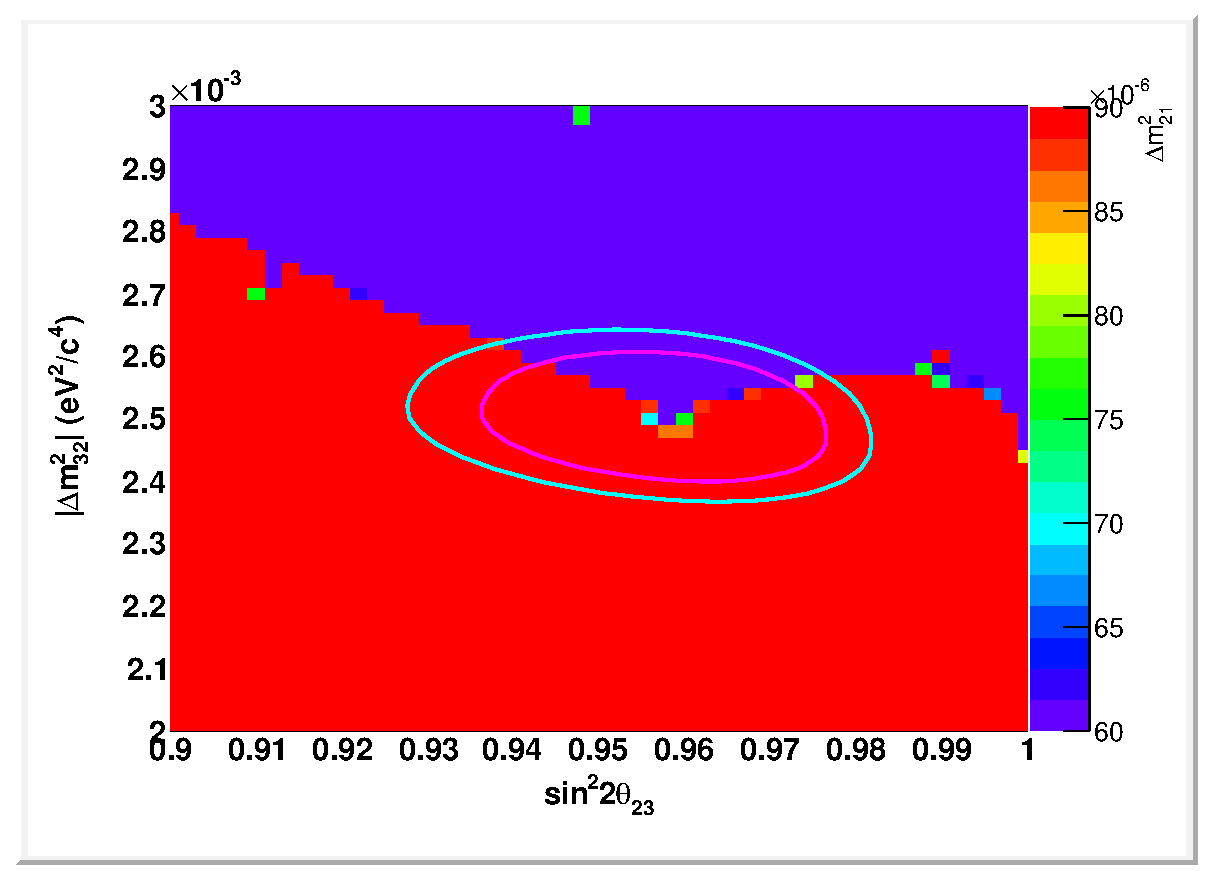
\includegraphics[width=0.5\textwidth]{images/validation/FittedDm12sqJointFitSolar.eps}
\caption{Fitted value of $sin^{2}2\theta_{12}$ (left) and  $\Delta m_{21}^{2}$ (right) for the joint oscillation analysis marginalizing the solar parameters for the estimated final POT. }
\label{fig:solarfit}
\end{center}
\end{figure}


%%%%%%%%%%%%%%%%%%%%
%%%% Delta CP %%%%%%%%%
\subsection{Further studies for $\delta_{CP}$}
\label{subsec:deltaCP}

From the results previously presented it is obvious that the parameter $\delta_{CP}$ needs a special treatment. In this subsection a careful discussion of the studies performed for $\delta_{CP}$ will follow.

As shown in figure \ref{fig:res2theta}  and in figure \ref{fig:res2thetacurroth} (bottom right plots), the distributions of residuals for the parameter $\delta_{CP}$ indicate that the fitter tends to fit the value of $\delta_{CP}$ at values 0 or multiples of $\pm \pi$. However from figure \ref{fig:1Dchisqdeltacp}, where the $\Delta\chi^{2}$ distribution is presented vs $\delta_{CP}$, it is clear that the differences in $\Delta\chi^{2}$ for the different values of $\delta_{CP}$ scanned, with any true input value of $\delta_{CP}$, are really tiny, of the order of $10^{-6}$ even at estimated final POT. This would mean in principle that our sensitivity to this parameter is very limited, being the indications of any preference of the fitter from figures \ref{fig:res2theta} and \ref{fig:res2thetacurroth} subject to that general tiny value of $\Delta\chi^{2}$ between any couple of values of $\delta_{CP}$. However, it will be the aim of this section to clarify if that is really the case under any assumption. 

One question that can be studied is the effect of the angle $\theta_{13}$ in the parameter $\delta_{CP}$, obviously related as those parameters appear together in the PMNS matrix (central term):

\begin{equation}
U = \left( \begin{array}{ccc} 1 & 0 & 0 \\  0 & c_{23} & s_{23} \\ 0 & -s_{23} & c_{23}\\ \end{array} \right) \times \left( \begin{array}{ccc}  c_{13} & 0 & s_{13}e^{-i\delta} \\ 0 & 1 & 0 \\ - s_{13}e^{i\delta} & 0 & c_{13}\\ \end{array} \right) \times \left( \begin{array}{ccc}  c_{12} & s_{12} & 0 \\ -s_{12} & c_{12} & 0 \\ 0 & 0 & 1\\ \end{array} \right)
\label{eq:PMNS}
\end{equation}

The following plot \ref{fig:dcpresconsttheta13} shows the effect of constraining the angle $sin^{2}\theta_{13}$ in the distribution of residuals for $\delta_{CP}$. This example plot was done with one of the sets used for the study of residuals, constraining the fitted value of the angle  $sin^{2}\theta_{13}$ to its true input value through a penalty term (described in equation \ref{eq:chisqconst} ) with an error of 20\%. It is shown in figure \ref{fig:dcpresconsttheta13} that constraining the fitted value of the angle $sin^{2}\theta_{13}$, the fitted value of $\delta_{CP}$ is automatically constrained as well, such that the second peak meaning a difference between the fitted value for $\delta_{CP}$ and its true value ($\delta_{CP}=0$ in this example) of $-\pi$ disappeared, remaining only one peak around zero for the residuals. 

 \begin{figure}[htbp]
\begin{center}
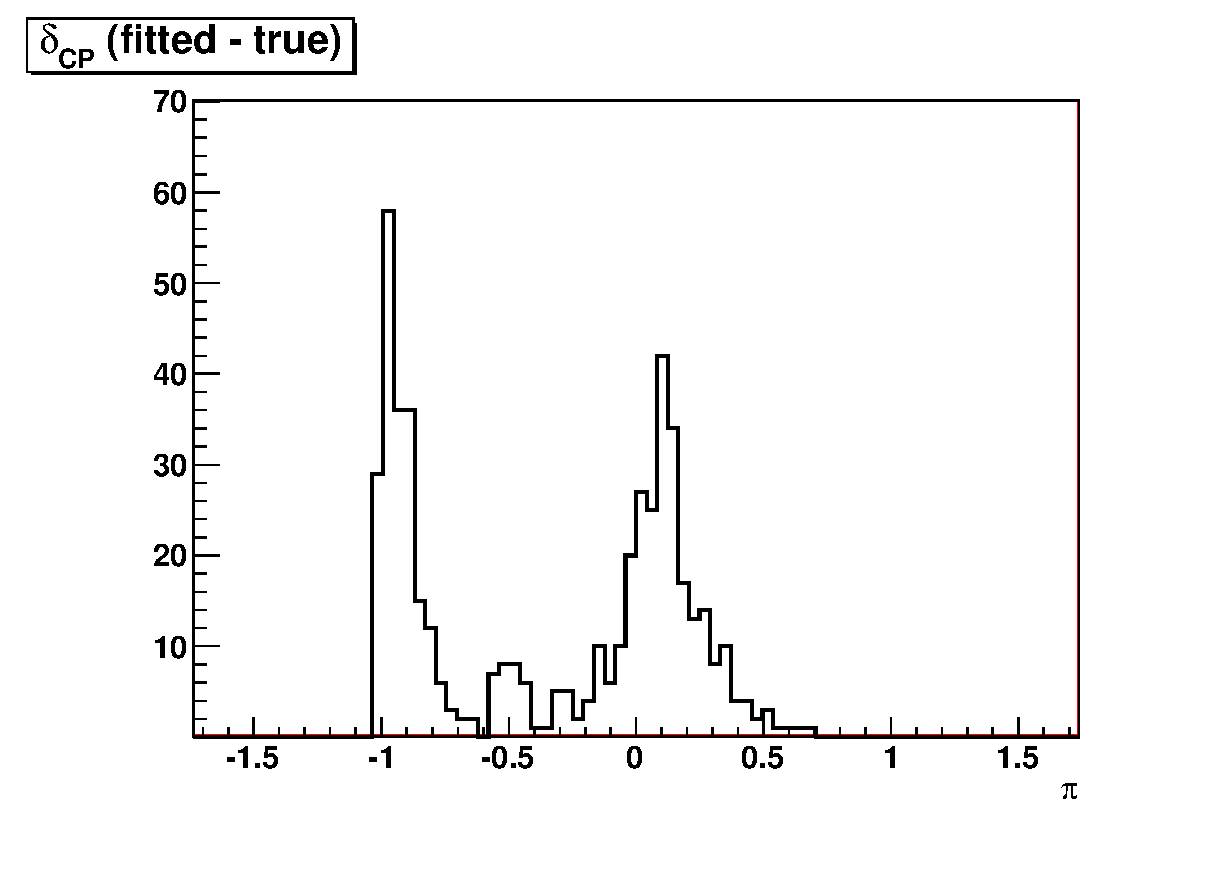
\includegraphics[width=0.5\textwidth]{images/validation/ResidualsDeltaCPSet4.eps}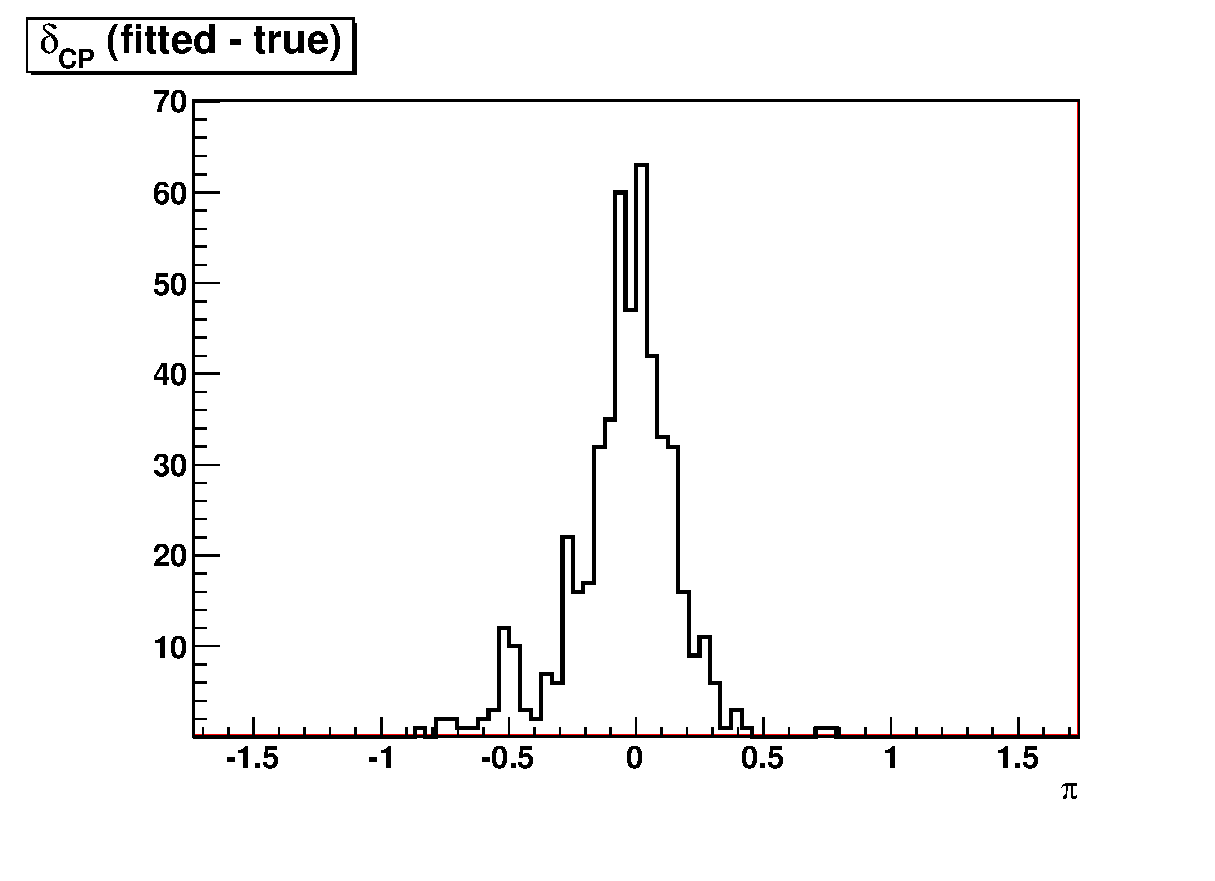
\includegraphics[width=0.5\textwidth]{images/validation/ResidualsDeltaCPSet4ConstrainTrue.eps}
\caption{Effect of constraining the angle $sin^{2}\theta_{13}$ in the distribution of residuals for $\delta_{CP}$ for the estimated final POT. On the left, the distribution of residuals for $\delta_{CP}$ before any constraint in the angle $sin^{2}\theta_{13}$, on the right the same distribution after constraining the angle $sin^{2}\theta_{13}$ with a 20\% error through a penalty term. }
\label{fig:dcpresconsttheta13}
\end{center}
\end{figure}

Another question to be addressed is the effect of systematics and the effect of the other oscillation parameters compared to the effect of the parameter $\delta_{CP}$ in terms of $\Delta\chi^{2}$. First of all it is necessary in order to compare to build the $\Delta\chi^{2}$ distribution vs $\delta_{CP}$ with no systematics and without fitting for the rest of oscillation parameters. Figure \ref{fig:chisqdcpnofits} shows the $\Delta\chi^{2}$ distribution vs $\delta_{CP}$ with no systematics and fixing the rest of oscillation parameters to the true input values used in the toy experiment (i.e. $sin^{2}\theta_{23}=0.56,|\Delta m_{32}^{2}|=2.4\times10^{-3}eV^{2}/c^{4},sin^{2}\theta_{13}=0.024$). The values of $\Delta\chi^{2}$ in figure \ref{fig:chisqdcpnofits} are much larger than observed in figure \ref{fig:1Dchisqdeltacp}, and a value of $\Delta\chi^{2} \approx 10$ is reached between $\delta_{CP}=0$ (minimum) and $\delta_{CP}=\pi/2$ (maximum). This seems to indicate that either the fitting of the rest of oscillation parameters or the fitting of systematics is hiding the actual picture merely due to the parameter $\delta_{CP}$. 

 \begin{figure}[htbp]
\begin{center}
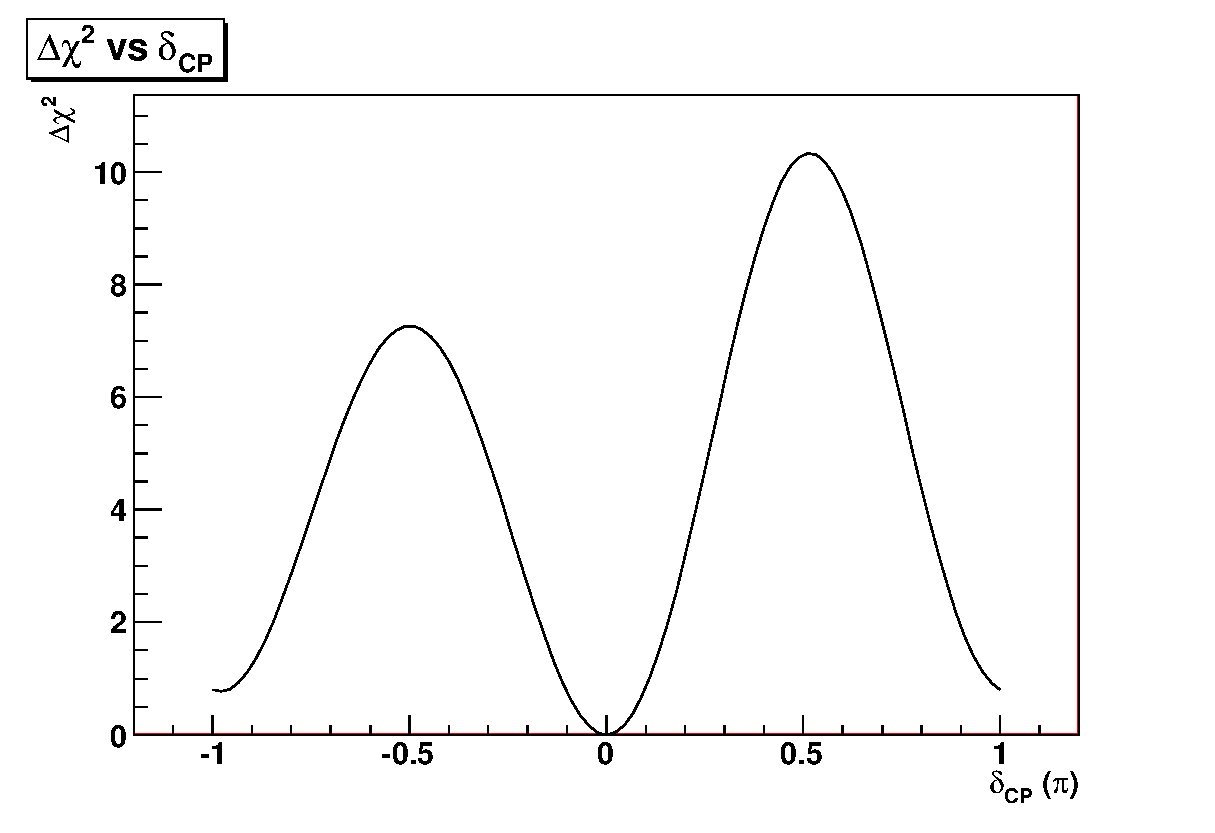
\includegraphics[width=0.5\textwidth]{images/validation/DeltaChisqVsDeltaCPNoSystNoOsc.eps}
\caption{$\Delta\chi^{2}$ distribution vs $\delta_{CP}$ with no systematics and fixing the rest of oscillation parameters to the true input values used in the toy experiment (i.e. $sin^{2}\theta_{23}=0.56,|\Delta m_{32}^{2}|=2.4\times10^{-3}eV^{2}/c^{4},sin^{2}\theta_{13}=0.024$) for the estimated final POT. The true input value for $\delta_{CP}$ is 0.}
\label{fig:chisqdcpnofits}
\end{center}
\end{figure}

In order to separate the effect of the other oscillation parameters and the effect of systematics in the $\Delta\chi^{2}$ distribution vs $\delta_{CP}$, the study done for figure \ref{fig:1Dchisqdeltacp} will be repeated for one example set of oscillation parameters ($sin^{2}\theta_{23}=0.56,|\Delta m_{32}^{2}|=2.4\times10^{-3}eV^{2}/c^{4},sin^{2}\theta_{13}=0.024,\delta_{CP}=0$) without fitting for systematics, but fitting for the other three oscillation parameters ($sin^{2}\theta_{23},|\Delta m_{32}^{2}|,sin^{2}\theta_{13}$). The result of such study is presented in figure \ref{fig:chisqdcpnosyst}. The new distribution shows that the values of $\Delta\chi^{2}$ decrease a lot in comparison with figure \ref{fig:chisqdcpnofits}, being of the order of $10^{-4}$ but still larger than the ones presented in figure \ref{fig:1Dchisqdeltacp} (top plot). This means that both the systematic errors and the other oscillation parameters are hiding the contribution of $\delta_{CP}$ to $\Delta\chi^{2}$ when being fitted. 

 \begin{figure}[htbp]
\begin{center}
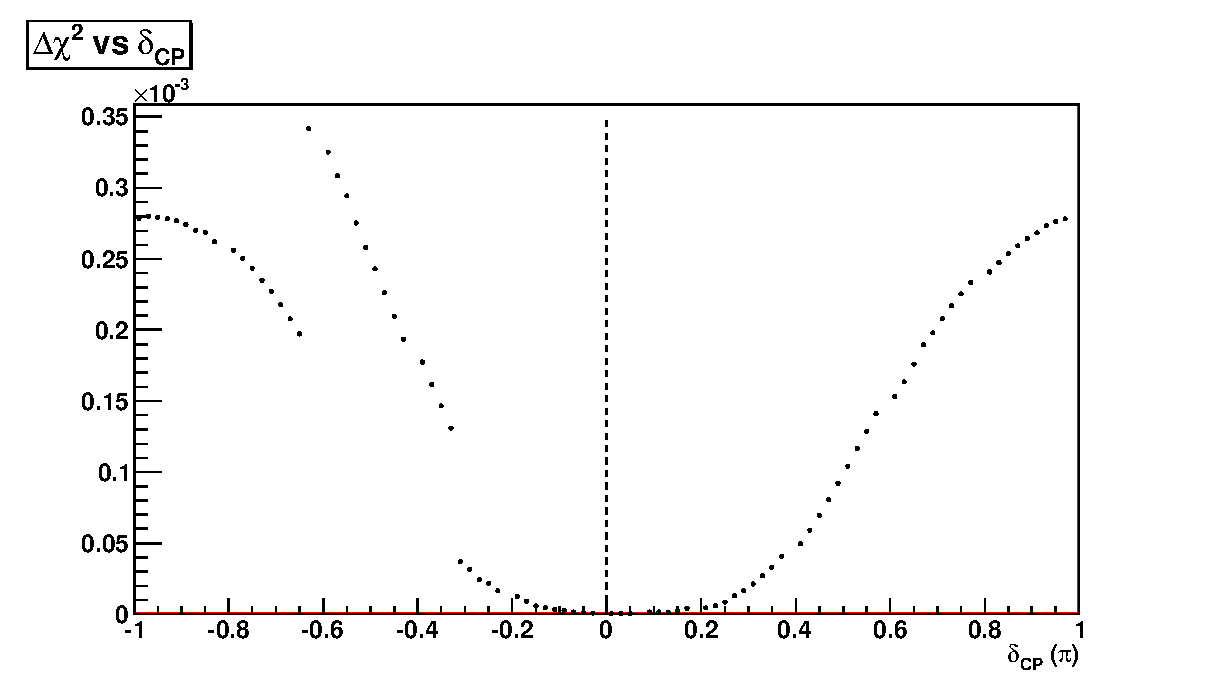
\includegraphics[width=0.5\textwidth]{images/validation/DeltaChisqVsDeltaCPNoSyst.eps}
\caption{$\Delta\chi^{2}$ distribution vs $\delta_{CP}$ without fitting for systematics but fitting for the rest of oscillation parameters ($sin^{2}\theta_{23},|\Delta m_{32}^{2}|,sin^{2}\theta_{13}$) for the estimated final POT.}
\label{fig:chisqdcpnosyst}
\end{center}
\end{figure}

Following the same idea as for residuals, the effect of constraining the angle $sin^{2}\theta_{13}$ can be also studied for the $\Delta\chi^{2}$ distribution vs $\delta_{CP}$. Figure \ref{fig:chisqdcpconsttheta13} shows the comparison between the $\Delta\chi^{2}$ distribution vs $\delta_{CP}$ for a true value of $\delta_{CP}=0$ and no constraints on the left and fixing $sin^{2}\theta_{13}$ to its true value on the right. Clearly, fixing the angle $sin^{2}\theta_{13}$ means ... 

 \begin{figure}[htbp]
\begin{center}

\includegraphics[width=0.2\textwidth]{images/placeholder.eps}
\caption{Comparison between the 1D $\Delta\chi^{2}$ distribution vs $\delta_{CP}$ for a true value of $\delta_{CP}=0$ and no constraints on the left and fixing $sin^{2}\theta_{13}$ to its true value on the right for the estimated final POT.}
\label{fig:chisqdcpconsttheta13}
\end{center}
\end{figure}

Now the effect of each systematic error on the $\Delta\chi^{2}$ distribution vs $\delta_{CP}$ will be studied. To do so the distribution of $\Delta\chi^{2}$ vs $\delta_{CP}$ was calculated with the rest of oscillation parameters fixed to the true values and tweaking each oscillation parameter to $+1\sigma$ (blue lines) and $-1\sigma$ (red lines), fixing the rest of systematics to 0. Figure \ref{fig:chisqdcpeachsyst} shows the result of such distributions of $\Delta\chi^{2}$ vs $\delta_{CP}$ fixing the rest of oscillation parameters to their true value, setting each oscillation parameter to  $+1\sigma$ (blue lines) and $-1\sigma$ (red lines) with the rest of systematic errors fixed to 0, compared to the distribution with all systematics set to 0 (black lines). With this figure \ref{fig:chisqdcpeachsyst} the effect of each systematic error can be studied in comparison with the effect of $\delta_{CP}$ itself in terms of $\Delta\chi^{2}$ by comparing the value of $\Delta\chi^{2}$ due to a change in $\delta_{CP}$ (measured from minimum to maximum, ~10) with the value of $\Delta\chi^{2}$ due to the change in each the systematic error (measured as the difference between black and blue/red lines in any point of $\delta_{CP}$). With these results it can be checked that some systematics do not produce any appreciable change in the $\Delta\chi^{2}$ distribution like the energy scale or the CCcoh/CCQE cross section ratio, while the effect of some others is comparable to the effect of the parameter itself, for instance the flux normalization or the CCother/CCQE cross section ratio. Also, it appears that the minimum value in $\delta_{CP}$ (that should be at 0) can be slightly biased as an effect of some systematic parameters like the flux normalization or the CCQE cross section.

 \begin{figure}[htbp]
\begin{center}
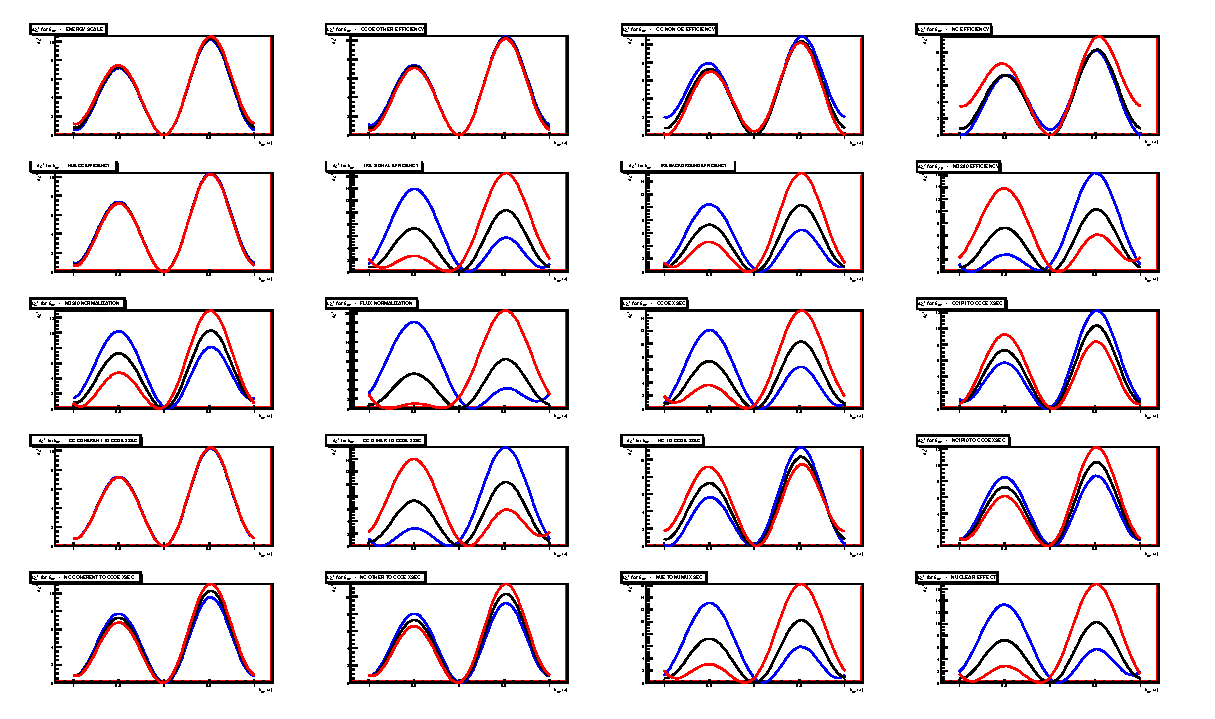
\includegraphics[width=1.0\textwidth,height=0.9\textheight]{images/validation/DeltaChisqVsDeltaCPSystStudy.eps}
\caption{$\Delta\chi^{2}$ distribution vs $\delta_{CP}$ fixing the rest of oscillation parameters to their true value, setting each oscillation parameter to  $+1\sigma$ (blue lines) and $-1\sigma$ (red lines) with the rest of systematic errors fixed to 0, compared to the distribution with all systematics set to 0 (black lines for the estimated final POT.}
\label{fig:chisqdcpeachsyst}
\end{center}
\end{figure}

Finally the effect of the parameter $\delta_{CP}$ in the confidence regions and contours can be also studied. Figure \ref{fig:effectdcpcontours} shows the comparison of the confidence regions result of the complete joint oscillation analysis marginalizing $\delta_{CP}$ and $sin^{2}\theta_{13}$ (solid lines) for the disappearance phase space, with the result of the joint oscillation analysis marginalizing only $sin^{2}\theta_{13}$ and fixing $\delta_{CP} = 0$ for the same disappearance phase space. From this plot it can be conclude that... 

 \begin{figure}[htbp]
\begin{center}

\includegraphics[width=0.2\textwidth]{images/placeholder.eps}
\caption{Comparison of the confidence regions for the disappearance phase space result of the complete joint oscillation analysis marginalizing $\delta_{CP}$ and $sin^{2}\theta_{13}$ (solid lines) with the result of the joint oscillation analysis marginalizing only $sin^{2}\theta_{13}$ and fixing $\delta_{CP} = 0$ for the estimated final POT.}
\label{fig:effectdcpcontours}
\end{center}
\end{figure}

From the results presented in this subsection it can be concluded that... Further studies will follow in the next joint oscillation analysis work once the effect of systematic errors will be reduced with the 2012 inputs. 



